% Copyright 2004 by Till Tantau <tantau@users.sourceforge.net>.
\documentclass{beamer}

\usetheme{Boadilla}

\usepackage{subfigure}
\usepackage{tikz}
\usepackage[export]{adjustbox}
\usepackage{wrapfig}
\usepackage{comment}
\usepackage{graphicx}
\usepackage{amsfonts}
\usepackage{xcolor}
\usepackage{amsmath}
\usepackage{amssymb}
\usepackage{algorithm2e}
\usepackage{algorithmic}
\usepackage{float}

\usetikzlibrary{datavisualization}
\usetikzlibrary{shapes,arrows,backgrounds}
\usetikzlibrary{intersections}
\usetikzlibrary{patterns}

\title[Diploma Thesis Presentation]{Distributed Training of Recurrent Neural Networks by FGM Protocol}

\author{Ilias Balampanis}

\institute[TUC]{ % (optional, but mostly needed)
School of Electrical and Computer Engineering \\
Technical University of Crete}

\pgfdeclareimage[height=1cm,width=1cm]{tuc-logo}{images/tuc_logo}
\logo{\pgfuseimage{tuc-logo}}

\setbeamertemplate{navigation symbols}{}

% Delete this block if you do not want the table of contents to pop up at the beginning of each subsection.
\AtBeginSubsection[]{
\begin{frame}
    <beamer>{Outline}
    \tableofcontents[currentsection,currentsubsection]
\end{frame}
}

% Let's get started
\begin{document}

    \begin{frame}
        \titlepage
    \end{frame}

    \begin{frame}{Outline}
        \tableofcontents
    \end{frame}

% Section and subsections will appear in the presentation overview and table of contents.
    \section{Background}\label{sec:background}
    \subsection{Machine Learning}\label{subsec:machine-learning}

\begin{frame}{Machine Learning (ML)}
    \setbeamertemplate{itemize items}[circle]
    \begin{itemize}
        \item{It is computational process for improving performance based on experience.}
        \vspace{0.3cm}
        \item{ML is a subfield of Artificial Intelligence (AI) and is primarily related to Data Analysis.}
        \vspace{0.3cm}
        \item{ML approaches are commonly divided into three ($3$) broad categories:
        \setbeamertemplate{itemize items}[square]
        \begin{itemize}
            \item Supervised Learning %(correct answers for each training point)
            \item Unsupervised Learning %("just make sense of the data")
            \item Reinforcement Learning %(reward sequence, no correct answers)
        \end{itemize}
        }
    \end{itemize}
\end{frame}

\begin{frame}{Neural Networks (NN)}
    \setbeamertemplate{itemize items}[circle]
    \begin{itemize}
        \item{A dominant class of ML algorithms.}
        \vspace{0.2cm}
        \item{ML with NN $\implies$ Deep Learning (DL)}
        \vspace{0.2cm}
        \item{Inspired by the neurophysiological experiments conducted by Hubel \& Wiesel in 1962.}
        \vspace{0.2cm}
        \item{Can approach highly complex functions and decision regions.}
        \vspace{0.2cm}
        \item[]{
        \begin{figure}[H]
            \centering
            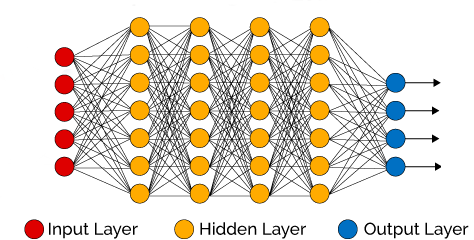
\includegraphics[width=8cm,height=3.8cm]{images/dnn.png}
            \caption{a Deep Neural Network.}
            \label{fig:dnn}
        \end{figure}}
    \end{itemize}
\end{frame}

\begin{frame}{NN learning process (1)}
    \setbeamertemplate{itemize items}[circle]
    \begin{itemize}
        \item{Assume a set $D=\{(x,y)\:|\:x\in\mathbb{R}^n,y\in\mathbb{N}\}$ of training data points.}
        \vspace{1cm}
        \item{A NN is a non-linear function $f$ parameterized by $w\in\mathbb{R}^d$.}
        \vspace{1cm}
        \item{Consider a globally continuous and differentiable \textbf{loss function} $\mathcal{L}:\mathcal{F}\times\mathcal{X}\times\mathcal{Y}\rightarrow\mathbb{R}_+$.}
    \end{itemize}
\end{frame}

\begin{frame}{NN learning process (2)}
    \setbeamertemplate{itemize items}[circle]
    \begin{itemize}
        \item{Training is performed by the mini-batch Gradient Descent (GD) algorithm
        \begin{itemize}
            \item[]{
            \begin{algorithm}[H]
                \begin{algorithmic}[1]
                    \WHILE{does not \emph{converge}}
                    \STATE \textbf{pick} randomly a mini-batch $\beta=\{(x_1,y_1),\dots,(x_{|\beta|},y_{|\beta|})\} \subset D$
                    \STATE \textbf{update} $w_{t+1}=w_t-\alpha\frac{1}{|\beta|}\sum_{i=1}^{|\beta|}\nabla_w\mathcal{L}(y_i,\hat{y_i})$
                    \ENDWHILE
                \end{algorithmic}
                \label{alg:gd}
            \end{algorithm}
            }
        \end{itemize}
        with $|\beta| \ll |D|$.
        }
        \vspace{0.3cm}
        \item{This process is called \textbf{back propagation}.}
    \end{itemize}
\end{frame}

\begin{frame}{Recurrent Neural Networks (RNN)}
    \setbeamertemplate{itemize items}[circle]
    \begin{itemize}
        \item{Introduced by David Rumelhart in 1986.}
        \vspace{0.2cm}
        \item{Can handle sequential data.}
        \vspace{0.2cm}
        \item{Considers the current input and also the previously received inputs.}
        \vspace{0.2cm}
        \item{Can memorize previous inputs due to its internal memory.}
        \vspace{0.2cm}
        \item[]{
        \begin{figure}[H]
            \centering
            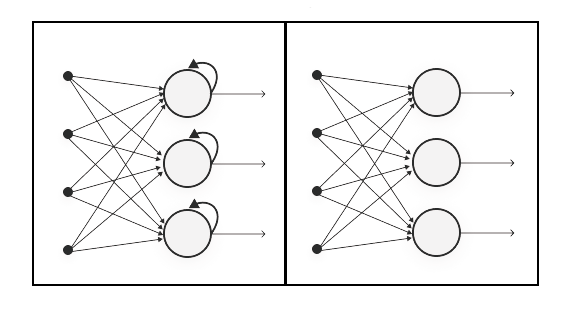
\includegraphics[width=7cm,height=3.5cm]{images/rnn-vs-fnn.png}
            \caption{a Recurrent Neural Network vs a Feed-forward one.}
            \label{fig:rnn-vs-fnn}
        \end{figure}
        }
    \end{itemize}
\end{frame}

\begin{frame}{LSTM Networks}
    \begin{columns}
        \column{0.55\textwidth}
        \setbeamertemplate{itemize items}[circle]
        \begin{itemize}
            \item{LSTM for Long Short Term Memory.}
            \vspace{0.2cm}
            \item{Not fundamentally different\\from RNN.}
            \vspace{0.2cm}
            \item{Use different functions to\\compute hidden state.}
            \vspace{0.2cm}
            \item{Cells decide what to keep in memory.}
            \vspace{0.2cm}
            \item{Very effective in capturing\\long term dependencies.}
        \end{itemize}
        \column{0.45\textwidth}
        \begin{figure}
            \subfigure[\tiny{The repeating module in a standard RNN contains a single layer.}]{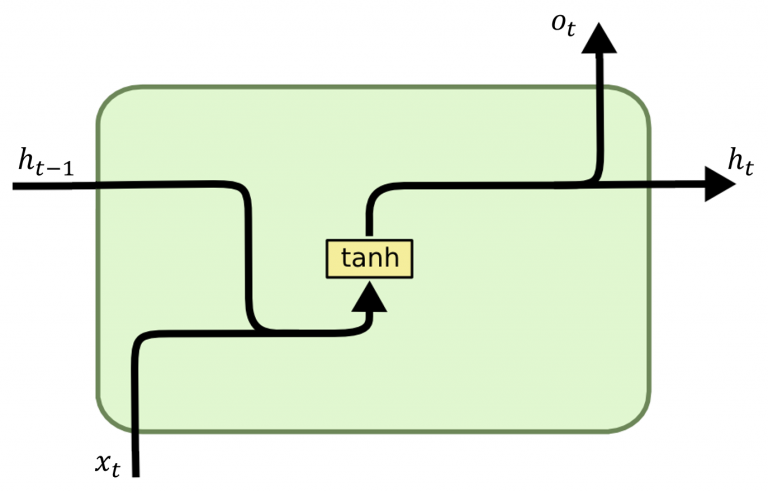
\includegraphics[width=3.8cm,height=2.5cm]{images/rnn.png}}
            \subfigure[\tiny{The repeating module in an LSTM contains four interacting layers.}]{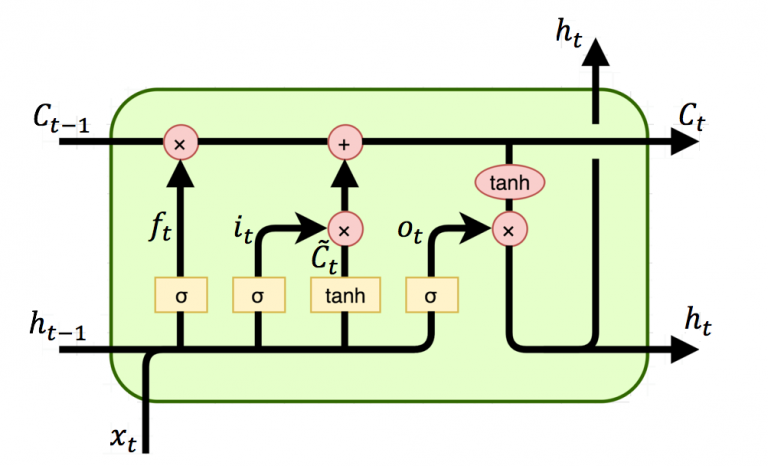
\includegraphics[width=3.8cm,height=2.5cm]{images/lstm.png}}
            \label{fig:rnn-vs-lstm}
        \end{figure}
    \end{columns}
\end{frame}

\begin{frame}{LSTM Networks Applications}
    \begin{columns}
        \column{0.55\textwidth}
        \setbeamertemplate{itemize items}[circle]
        \begin{itemize}
            \item{Time series prediction}
            \vspace{0.5cm}
            \item{Speech recognition}
            \vspace{0.5cm}
            \item{Handwriting recognition}
            \vspace{0.5cm}
            \item{Short-term traffic forecast}
        \end{itemize}
        \column{0.45\textwidth}
        \begin{figure}
            \subfigure{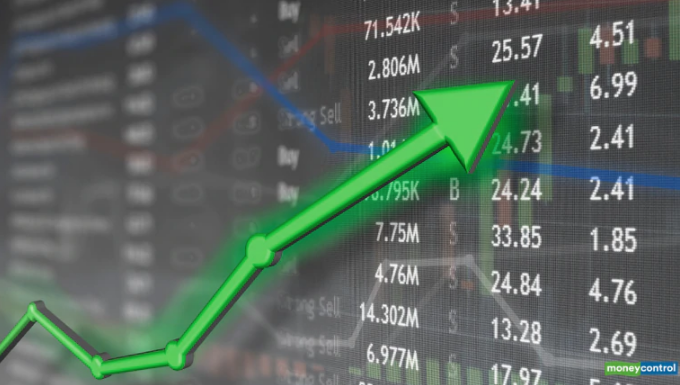
\includegraphics[width=4cm,height=2.5cm,center]{images/stocks.png}}
            \subfigure{
\includegraphics[width=4cm,height=2.5cm,center]{images/speech-recgn.png}}
            \label{fig:apps}
        \end{figure}
    \end{columns}
\end{frame}

\subsection{Distributed Deep Learning}\label{subsec:distributed-deep-learning}

\begin{frame}{Network Architecture}
    \begin{columns}
        \column{0.5\textwidth}
        \setbeamertemplate{itemize items}[circle]
        \begin{itemize}
            \item{A \textbf{star network} topology with
            \setbeamertemplate{itemize items}[square]
            \begin{itemize}
                \item a \emph{parameter server}
                \item $n$ \emph{workers}
            \end{itemize}}
            \vspace{0.2cm}
            \item{Each worker $i \in [\,1,n]\,$ has a chunk $D_i$ of the whole training set $D$.}
            \vspace{0.2cm}
            \item{Each worker has a \textbf{replica} of the DL model.}
        \end{itemize}
        \column{0.5\textwidth}
        \begin{figure}
            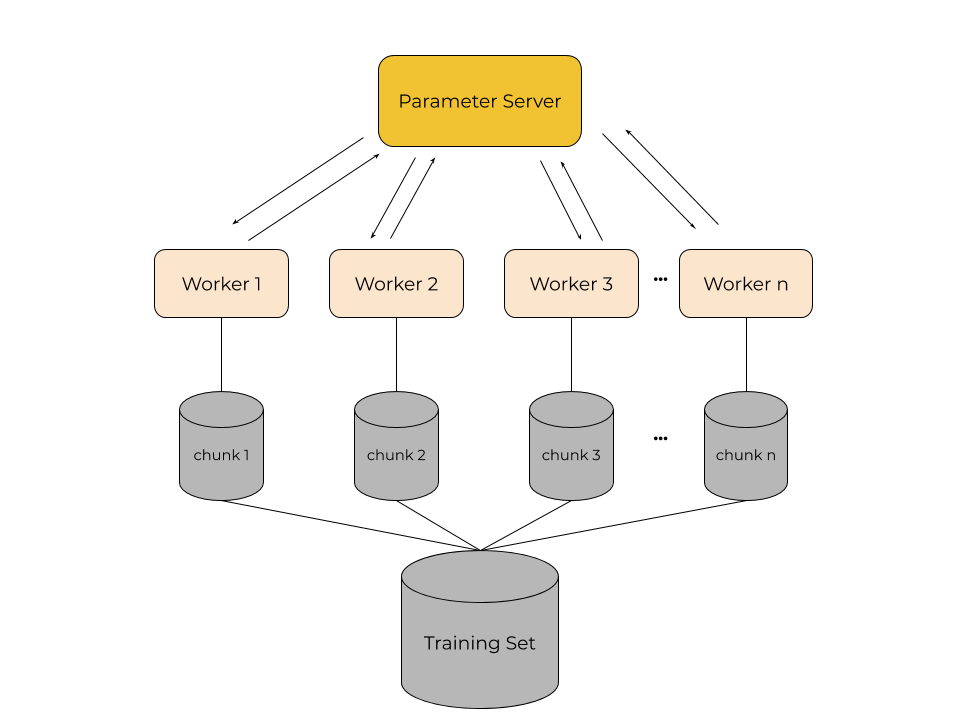
\includegraphics[width=8.5cm,height=6cm,center]{images/parameter-server.png}\label{fig:param-server}
        \end{figure}
    \end{columns}
\end{frame}

\begin{frame}{Parameter Server (PS) model (1)}
    \setbeamertemplate{itemize items}[circle]
    \begin{itemize}
        \item{The most known model for distributed DL.}
        \vspace{1cm}
        \item{The number of rounds is \textbf{fixed} ($r = \frac{|D|}{n \cdot |\beta|}$).}
        \vspace{1cm}
        \item{The network cost is also \textbf{fixed} ($C_{PS} = \frac{|D|}{|\beta|} \cdot 2 \cdot C_{model}$).}
    \end{itemize}
\end{frame}

\begin{frame}{Parameter Server (PS) model (2)}
    \setbeamertemplate{itemize items}[circle]
    \begin{itemize}
        \item{\textbf{Pseudo algorithm}
        \begin{algorithm}[H]
            \vspace{0.5cm}
            \begin{algorithmic}[1]
                \STATE The PS initializes the parameters of the DL model.
                \STATE The PS broadcasts the model parameters to each worker.
                \STATE Each worker fits a mini-batch, taken from its chunk, using the mini-batch GD algorithm.
                \STATE When \textbf{step 3} is done, all workers send their model parameters\\to the PS where the aggregation takes place.
                \STATE While each chunk is not empty, go to \textbf{step 2}, otherwise \textbf{all done}.
            \end{algorithmic}
            \label{alg:param-server}
        \end{algorithm}
        }
    \end{itemize}
\end{frame}

\begin{frame}{The environment of the Geometric Monitoring (GM) protocol}
    \begin{columns}
        \column{0.5\textwidth}
        \setbeamertemplate{itemize items}[circle]
        \begin{itemize}
            \item{A \textbf{star network} topology with
            \setbeamertemplate{itemize items}[square]
            \begin{itemize}
                \item $n$ workers with a \textbf{replica} of the DL model, $\pmb{W}_i$.
                \item a coordinator that holds $\pmb{E}\in\mathbb{R}^d$ an estimate of $\pmb{W}(t)=\frac{1}{n}\sum_{i=1}^n\pmb{W}_i(t)$.
            \end{itemize}}
            \vspace{0.1cm}
            \item{Each worker $i \in [\,1,n]\,$ has a chunk $D_i$ of the whole training set $D$.}
            \vspace{0.1cm}
            \item{It is surely more efficient than the PS classic model regarding the network traffic.}
        \end{itemize}
        \column{0.5\textwidth}
        \begin{figure}
            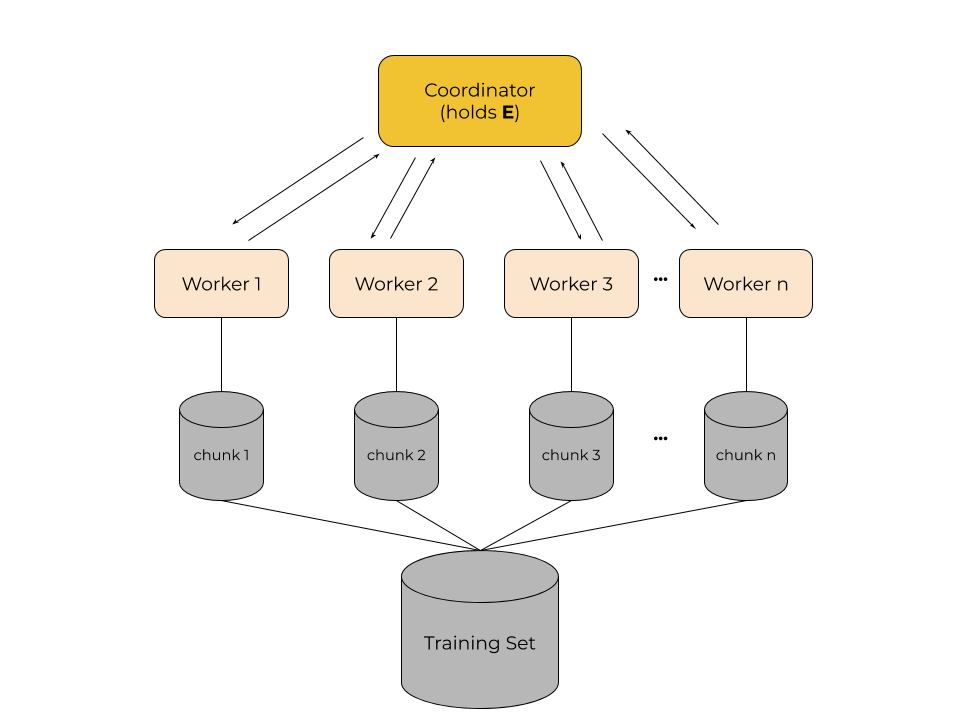
\includegraphics[width=8cm,height=6.5cm,center]{images/ml-fgm.png}\label{fig:ml-gm}
        \end{figure}
    \end{columns}
\end{frame}

\begin{frame}{Definitions}
    \setbeamertemplate{itemize items}[circle]
    \begin{itemize}
        \item{Introduced for DL purposes by Michael Kamp et al. (2014).\\\lbrack Dynamic Model Synchronization (DMS)\rbrack}
    \end{itemize}
    \begin{columns}
        \column{0.5\textwidth}
        \vspace{-0.5cm}
        \setbeamertemplate{itemize items}[square]
        \begin{itemize}
            \item[]{
            \begin{block}{Model parameters Estimate}
                $\pmb{E}=\frac{1}{n}\sum\pmb{W}_i(t)$
            \end{block}
            \begin{block}{Admissible region}
                $A=\{\pmb{W}\in\mathbb{R}^d\:\:|\:\:||\pmb{W}-\pmb{E}||_2^2 - T\leq 0\}$
                \centering
                \newline
                $A$ is \textbf{convex}
            \end{block}
            \begin{block}{Safe function for $A$}
                $\phi(\pmb{W},\pmb{E}) = ||\pmb{W}-\pmb{E}||_2^2 - T$
            \end{block}
            }
        \end{itemize}
        \column{0.45\textwidth}
        \vspace{-0.2cm}
        \begin{block}{Local model parameters\\(Drift Vector)}
            $\pmb{W}_i(t)=\pmb{\Delta W}_i(t)+\pmb{E}$
        \end{block}
        \hspace{0.75cm}
        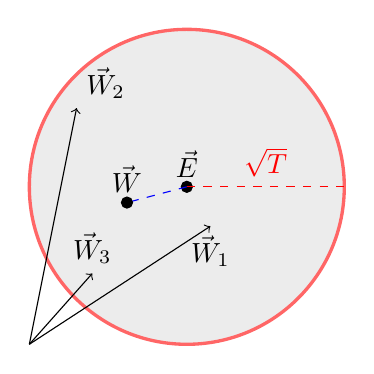
\begin{tikzpicture}
            \filldraw[color=red!60, fill=gray!50, fill opacity=0.3, very thick](0,0) circle (2);
            \coordinate (E) at (0,0);
            \coordinate (u1) at (0.3,-0.5);
            \coordinate (u2) at (-1.4,1.0);
            \coordinate (u3) at (-1.2,-1.1);
            \draw [fill] (E) circle (0.2em) node [anchor=south] {$\vec{E}$};
            \draw [->,thin] (-2,-2)--(u1)  node [anchor=north]{$\vec{W}_1$};
            \draw [->,thin] (-2,-2)--(u2) node [anchor=south west] {$\vec{W}_2$};
            \draw [->,thin] (-2,-2)--(u3) node [anchor=south]
            {$\vec{W}_3$};
            \coordinate (x) at (-0.76,-0.2);
            \draw [blue,dashed] (E)--(x);
            \draw [fill] (x) circle (0.2em) node [anchor=south] {$\vec{W}$};
            \draw [red,dashed] (E)--(2,0) node [pos=0.5, anchor=south] {$\sqrt{T}$};
        \end{tikzpicture}
        \vspace{-0.5cm}\hspace{1cm}$\forall i,\pmb{W}_i\in A \Rightarrow\pmb{W}\in A$
    \end{columns}
\end{frame}

\begin{frame}{The GM Protocol (1)}
    \begin{columns}
        \column{0.5\textwidth}
        \vspace{-3cm}
        \setbeamertemplate{itemize items}[circle]
        \begin{itemize}
            \item{At the \textbf{beginning} of a round,
            \vspace{0.2cm}
            \setbeamertemplate{itemize items}[square]
            \begin{itemize}
                \item{The coordinator knows the model parameters from all workers $\pmb{W}_i$.}
            \end{itemize}
            }
        \end{itemize}
        \column{0.5\textwidth}
        \begin{figure}
            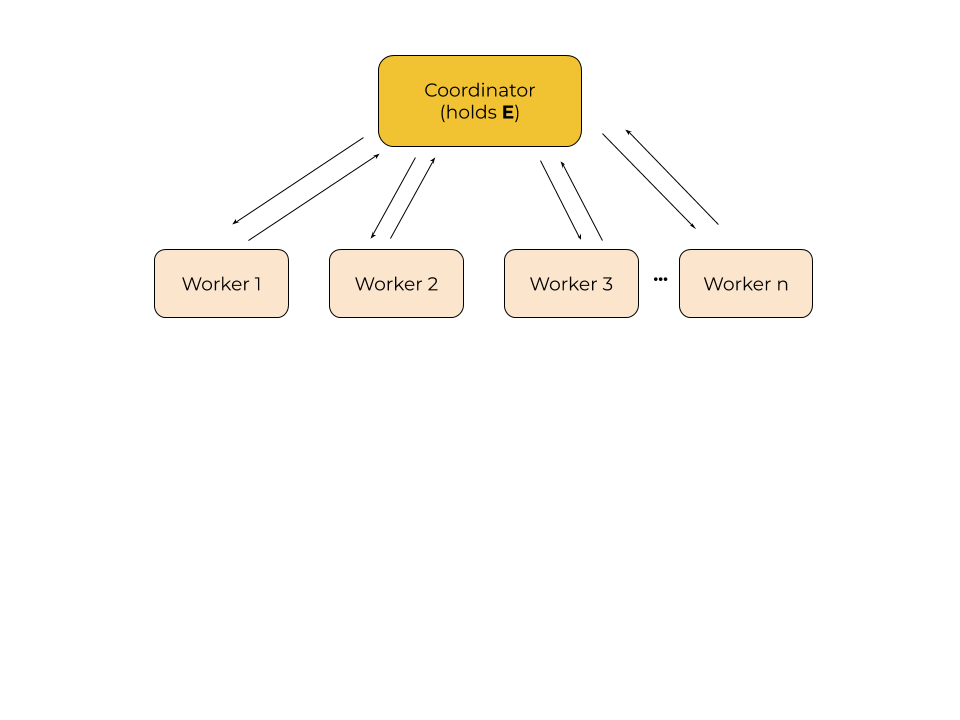
\includegraphics[width=8.5cm,height=6cm,center]{images/ml-fgm-2.png}\label{fig:ml-gm-1}
        \end{figure}
    \end{columns}
    \vspace{-3cm}
    \setbeamertemplate{itemize items}[circle]
    \begin{itemize}
        \item[]{
        \setbeamertemplate{itemize items}[square]
        \begin{itemize}
            \item{The coordinator sends the estimate $\pmb{E}$ to all workers.}
            \vspace{0.3cm}
            \item{Each worker initializes the parameters $\pmb{W}_i=\pmb{E}$.}
        \end{itemize}
        }
    \end{itemize}
\end{frame}

\begin{frame}{The GM Protocol (2)}
    \begin{columns}
        \column{0.5\textwidth}
        \vspace{-3cm}
        \setbeamertemplate{itemize items}[circle]
        \begin{itemize}
            \item{\textbf{During} a round,
            \vspace{0.2cm}
            \setbeamertemplate{itemize items}[square]
            \begin{itemize}
                \item{Each worker updates $\pmb{W}_i$ by fitting a batch of samples.}
                \vspace{0.3cm}
                \item{Next, each worker calculates its drift vector $\pmb{X}_i$.}
            \end{itemize}
            }
        \end{itemize}
        \column{0.5\textwidth}
        \begin{figure}
            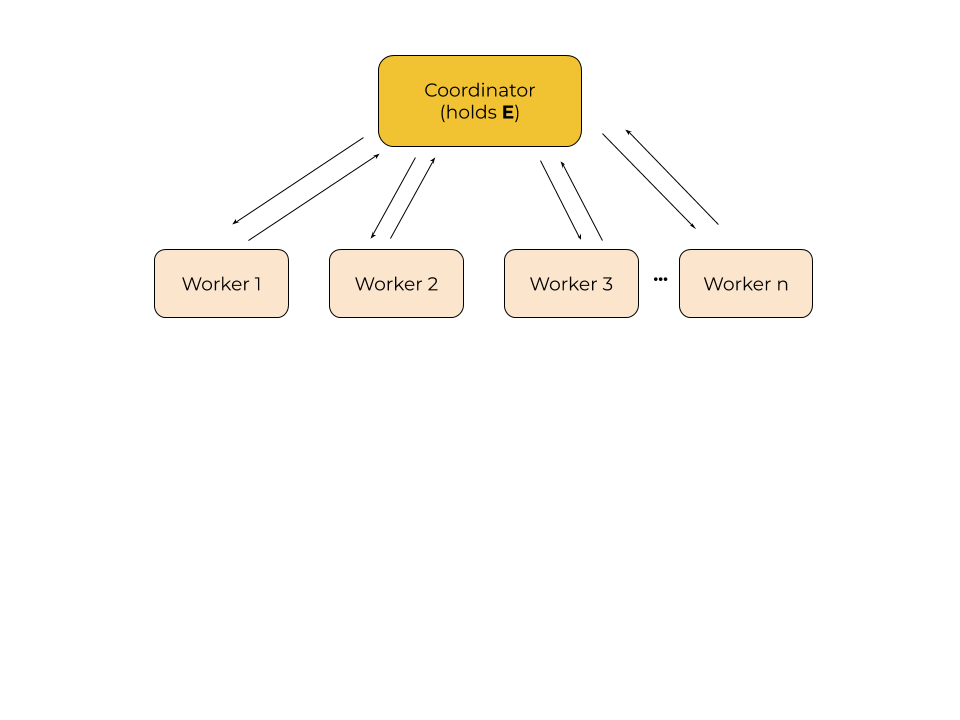
\includegraphics[width=8.5cm,height=6cm,center]{images/ml-fgm-2.png}\label{fig:ml-gm-2}
        \end{figure}
    \end{columns}
    \vspace{-3cm}
    \setbeamertemplate{itemize items}[circle]
    \begin{itemize}
        \item[]{
        \setbeamertemplate{itemize items}[square]
        \begin{itemize}
            \item{Each worker checks that $\pmb{W}_i\in A\Rightarrow||\pmb{W}_i(t)-\pmb{E}||_2^2 - T \leq 0$.}
            \vspace{0.3cm}
            \item{If $\pmb{W}_i\not\in A$ occurs at a worker, then sends a \textbf{local violation} message to the coordinator.}
        \end{itemize}
        }
    \end{itemize}
\end{frame}

\begin{frame}{The GM Protocol (3)}
    \begin{columns}
        \column{0.5\textwidth}
        \vspace{-3cm}
        \setbeamertemplate{itemize items}[circle]
        \begin{itemize}
            \item{At the \textbf{end} of a round\\(\emph{the coordinator receives a local violation message}),
            \vspace{0.2cm}
            \setbeamertemplate{itemize items}[square]
            \begin{itemize}
                \item{The coordinator receives from each worker for the\\current $\pmb{W}_i$.}
            \end{itemize}
            }
        \end{itemize}
        \column{0.5\textwidth}
        \begin{figure}
            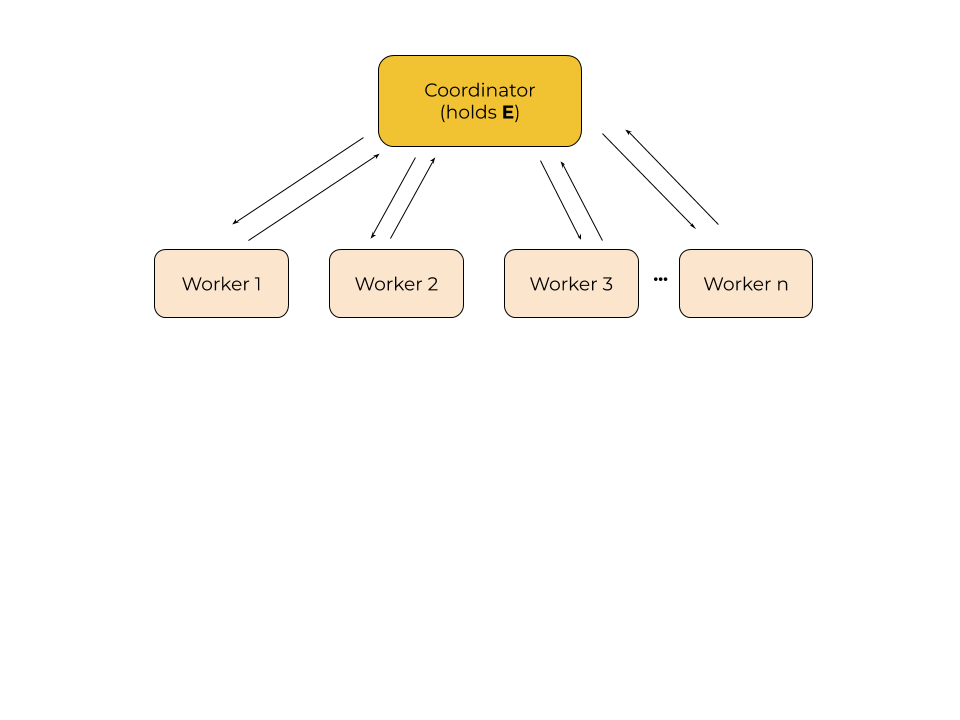
\includegraphics[width=8.5cm,height=6cm,center]{images/ml-fgm-2.png}\label{fig:ml-gm-3}
        \end{figure}
    \end{columns}
    \vspace{-3cm}
    \setbeamertemplate{itemize items}[circle]
    \begin{itemize}
        \item[]{
        \setbeamertemplate{itemize items}[square]
        \begin{itemize}
            \item{The coordinator calculates the new estimate ($\pmb{E}$).}
        \end{itemize}
        }
    \end{itemize}
\end{frame}

%\begin{frame}{Conditions}
%    \setbeamertemplate{itemize items}[circle]
%    \begin{itemize}
%        \item{Uses the conditions which introduced by Keren et al. (2006).}
%        \vspace{0.4cm}
%        \item{The protocol totally monitors the \textbf{variance} of the distributed parameter vectors,
%        \[\frac{1}{n}\sum_{i=1}^n||\pmb{W}_i(t)-\pmb{W}(t)||_2^2 \leq \frac{1}{n}\sum_{i=1}^n||\pmb{W}_i(t)-\pmb{E}||_2^2 - T \leq 0.\]}
%        \vspace{-0.4cm}
%        \item{Each worker checks its \textbf{local condition},
%        \[\forall i,||\pmb{W}_i(t)-\pmb{E}||_2^2 - T \leq 0.\]}
%    \end{itemize}
%\end{frame}

    \section{Implementation}\label{sec:implementation}
    \subsection{Deep Learning using Functional Geometric Monitoring (FGM) protocol}\label{subsec:deep-learning-using-fgm-protocol}

\begin{frame}{Definitions}
    \begin{block}{Definition (Safe function for admissible region $A$)}
        A function $\phi :\mathbb{R}^d\rightarrow \mathbb{R}$ such that, for every $n$, and every $\pmb{X}_i$, i \in [\,1,n]\,\\
        \vspace{0.1cm}
        \begin{center}
            $\sum_{i=1}^n\phi (\pmb{W}_i) \leq 0$\hspace{0.4cm}$\Longrightarrow$\hspace{0.4cm}$\frac{1}{n}\sum_{i=1}^n\pmb{W}_i\in A$
        \end{center}
    \end{block}
    \vspace{0.4cm}
    \begin{columns}
        \column{0.65\textwidth}
        \begin{itemize}
            \item[]{The FGM protocol [Samoladas et al. 2018] monitors the condition $\sum_{i=1}^n\phi (\pmb{W}_i) \leq 0$.}
        \end{itemize}
        \column{0.35\textwidth}
        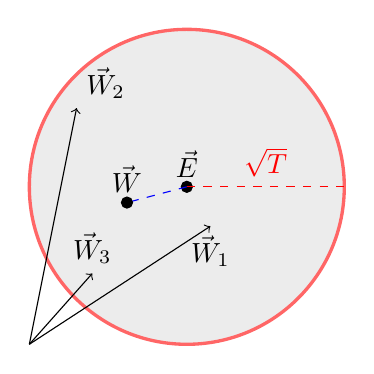
\begin{tikzpicture}
            \filldraw[color=red!60, fill=gray!50, fill opacity=0.3, very thick](0,0) circle (2);
            \coordinate (E) at (0,0);
            \coordinate (u1) at (0.3,-0.5);
            \coordinate (u2) at (-1.4,1.0);
            \coordinate (u3) at (-1.2,-1.1);
            \draw [fill] (E) circle (0.2em) node [anchor=south] {$\vec{E}$};
            \draw [->,thin] (-2,-2)--(u1)  node [anchor=north]{$\vec{W}_1$};
            \draw [->,thin] (-2,-2)--(u2) node [anchor=south west] {$\vec{W}_2$};
            \draw [->,thin] (-2,-2)--(u3) node [anchor=south]
            {$\vec{W}_3$};
            \coordinate (x) at (-0.76,-0.2);
            \draw [blue,dashed] (E)--(x);
            \draw [fill] (x) circle (0.2em) node [anchor=south] {$\vec{W}$};
            \draw [red,dashed] (E)--(2,0) node [pos=0.5, anchor=south] {$\sqrt{T}$};
        \end{tikzpicture}
    \end{columns}
\end{frame}

\begin{frame}{Correspondence with GM protocol}
    \setbeamertemplate{itemize items}[circle]
    \begin{itemize}
        \item{The \textbf{admissible region} in GM protocol (M. Kamp) is the \textbf{convex set}
        \newline
        \begin{center}
            $A=\{\pmb{W}_i\in\mathbb{R}^d\:\:|\:\:||\pmb{W}_i-\pmb{E}||_2^2 - T \leq 0\}$
        \end{center}
        }
        \vspace{0.4cm}
        \item{Samoladas et al. constructed the concave function $\phi:\mathbb{R}^d\rightarrow\mathbb{R}$ that is safe for $A$ as
        \newline
        \begin{center}
            $\phi(\pmb{W_i},\pmb{E}) = \max\{-T||\pmb{E}|| - \pmb{W_i}\frac{\pmb{E}}{\pmb{||E||}}, ||\pmb{W_i}+\pmb{E}|| - (1+T)||\pmb{E}||\}$
        \end{center}
        We can call this function as \textbf{’spherical cap’}.
        }
        \vspace{0.4cm}
        \item{Finally, the coordinator monitors the condition,
        \newline
        \begin{center}
            $\sum_{i=1}^n\phi(\pmb{W}_i,\pmb{E}) \leq 0$
        \end{center}
        }
    \end{itemize}
\end{frame}

\begin{frame}{The FGM Protocol (1)}
    \begin{columns}
        \column{0.5\textwidth}
        \setbeamertemplate{itemize items}[circle]
        \begin{itemize}
            \item{At the \textbf{beginning} of a round,
            \vspace{0.2cm}
            \setbeamertemplate{itemize items}[square]
            \begin{itemize}
                \item{The coordinator knows the model parameters from all workers $\pmb{W}_i$.}
                \vspace{0.3cm}
                \item{The coordinator ships the estimate $\pmb{E}$ to all workers.}
                \vspace{0.3cm}
                \item{Each site calculates $\phi$ from $\pmb{E}$.}
                \vspace{0.3cm}
                \item{Each site initializes $\pmb{W}_i=\pmb{E}$.}
            \end{itemize}
            }
        \end{itemize}
        \column{0.5\textwidth}
        \begin{figure}
            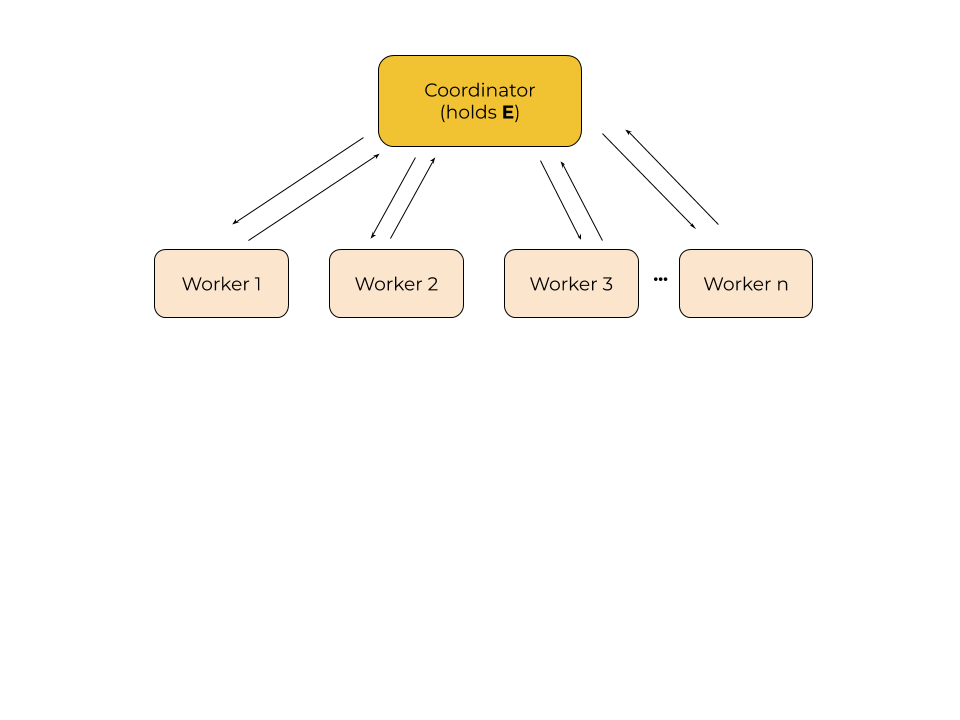
\includegraphics[width=8.5cm,height=6cm,center]{images/ml-fgm-2.png}\label{fig:ml-fgm-1}
        \end{figure}
    \end{columns}
\end{frame}

\begin{frame}{The FGM Protocol (2)}
    \begin{columns}
        \column{0.5\textwidth}
        \vspace{-1cm}
        \setbeamertemplate{itemize items}[circle]
        \begin{itemize}
            \item{\textbf{During} a round,
            \vspace{0.2cm}
            \setbeamertemplate{itemize items}[square]
            \begin{itemize}
                \item{Each worker updates $\pmb{W}_i$ by fitting a batch of samples.}
                \vspace{0.3cm}
                \item{The coordinator monitors the following condition,\\
                \begin{center}
                    $\psi = \sum_{i=1}^n\phi(\pmb{W}_i,\pmb{E}) \leq 0$
                \end{center}
                }
            \end{itemize}
            }
        \end{itemize}
        \column{0.5\textwidth}
        \begin{figure}
            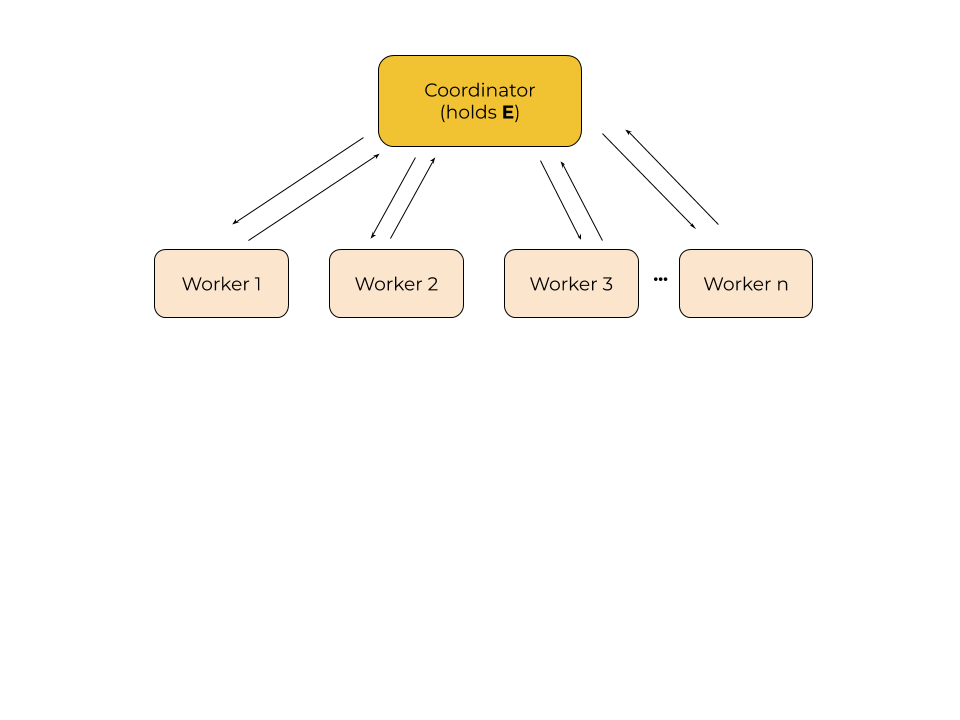
\includegraphics[width=8.5cm,height=6cm,center]{images/ml-fgm-2.png}\label{fig:ml-fgm-2}
        \end{figure}
    \end{columns}
\end{frame}

\begin{frame}{The FGM Protocol (3)}
    \begin{columns}
        \column{0.5\textwidth}
        \vspace{-1cm}
        \setbeamertemplate{itemize items}[circle]
        \begin{itemize}
            \item{At the \textbf{end} of a round,
            \vspace{0.2cm}
            \setbeamertemplate{itemize items}[square]
            \begin{itemize}
                \item{The coordinator receives from each worker the current $\pmb{X}_i$.}
                \vspace{0.3cm}
                \item{The coordinator calculates the new estimate ($\pmb{E}$) and quantum ($\pmb{\theta}$).}
            \end{itemize}
            }
        \end{itemize}
        \column{0.5\textwidth}
        \begin{figure}
            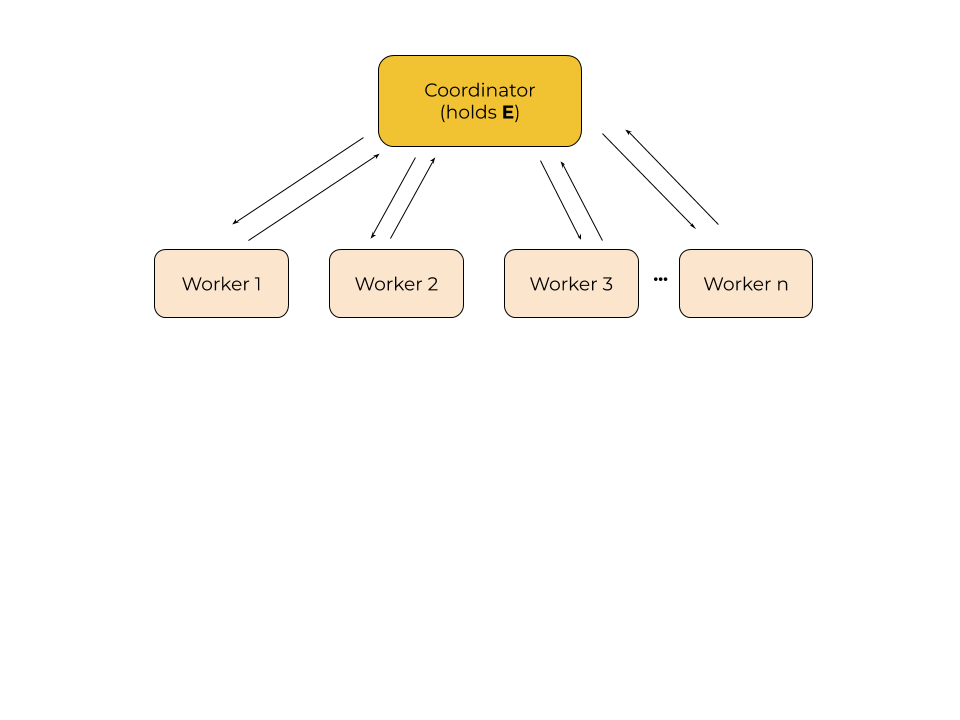
\includegraphics[width=8.5cm,height=6cm,center]{images/ml-fgm-2.png}\label{fig:ml-fgm-3}
        \end{figure}
    \end{columns}
\end{frame}

\begin{frame}{Contribution}
    \setbeamertemplate{itemize items}[circle]
    \begin{itemize}
        \item{Michael Kamp et al. had not tested their method in this type of NNs.}
        \vspace{1cm}
        \item{We attempt to train these difficult networks distributedly by a more efficient method.}
    \end{itemize}
\end{frame}

    \section{Experimental Results}\label{sec:experimental-results}
    \subsection{Protocols Comparison}\label{subsec:protocols-comparison}

\begin{frame}{Experiments Setup}
    \setbeamertemplate{itemize items}[circle]
    \begin{itemize}
        \item{\textbf{Quantities} that we care for
        \setbeamertemplate{itemize items}[square]
        \begin{itemize}
            \item{ML model prediction \textbf{accuracy}}
            \item{number of \textbf{rounds} of each protocol}
            \item{network \textbf{traffic} in bytes that each protocol needed to perform}
        \end{itemize}
        }
        \vspace{0.2cm}
        \item{The experiments conducted for \textbf{various}
        \setbeamertemplate{itemize items}[square]
        \begin{itemize}
            \item{thresholds ($\pmb{T}$)}
            \item{mini-batch sizes ($\pmb{|\beta|}$)}
            \item{number of workers ($\pmb{n}$)}
        \end{itemize}
        }
        \vspace{0.2cm}
        \item{Both datasets cut into $\pmb{n}$ chunks.}
        \vspace{0.2cm}
        \item{The working load allocated \textbf{uniformly} to each worker.}
    \end{itemize}
\end{frame}

\begin{frame}{Machine Learning Problems (1)}
    \setbeamertemplate{itemize items}[circle]
    \begin{itemize}
        \item{We compare the two protocols in \textbf{two} distinct ML problems using the \textbf{same safe function} (spherical cap).}
        \vspace{0.3cm}
        \item{\textbf{Problem 1} - Classification
        \vspace{0.1cm}
        \setbeamertemplate{itemize items}[square]
        \begin{itemize}
            \item{\textbf{Dataset:} San Francisco Crime Classification (SFCC)}
            \vspace{0.1cm}
            \item{\textbf{Features:} $9$}
            \vspace{0.1cm}
            \item{\textbf{Classes:} $39$}
            \vspace{0.1cm}
            \item{\textbf{Dataset size:} $878,049$ data points}
            \vspace{0.1cm}
            \item{The \textbf{goal} is to predict the category of crime that occurred, given the time and location and the rest of
            variables.}
        \end{itemize}
        }
    \end{itemize}
\end{frame}

\begin{frame}{Machine Learning Problems (2)}
    \setbeamertemplate{itemize items}[circle]
    \begin{itemize}
        \item{\textbf{Problem 2} - Natural Language Processing (NLP)
        \vspace{0.1cm}
        \setbeamertemplate{itemize items}[square]
        \begin{itemize}
            \item{\textbf{Dataset:} Amazon Fine Food Reviews (AFFR)}
            \vspace{0.2cm}
            \item{\textbf{Max input words:} $200$}
            \vspace{0.2cm}
            \item{\textbf{Classes:} $2$}
            \vspace{0.2cm}
            \item{\textbf{Dataset size:} $568,454$ data points}
            \vspace{0.2cm}
            \item{The \textbf{goal} is to predict if the given review is positive or negative\\\textbf{(Sentiment Analysis)}.}
        \end{itemize}
        }
    \end{itemize}
\end{frame}

\begin{frame}{Results (1) - Changing the threshold ($\pmb{T}$)}
    \begin{itemize}
        \centering
        \item[]{\lbrack mini-batch=$16$, workers=$8$\rbrack}
    \end{itemize}
    \vspace{-0.3cm}
    \begin{figure}
        \subfigure{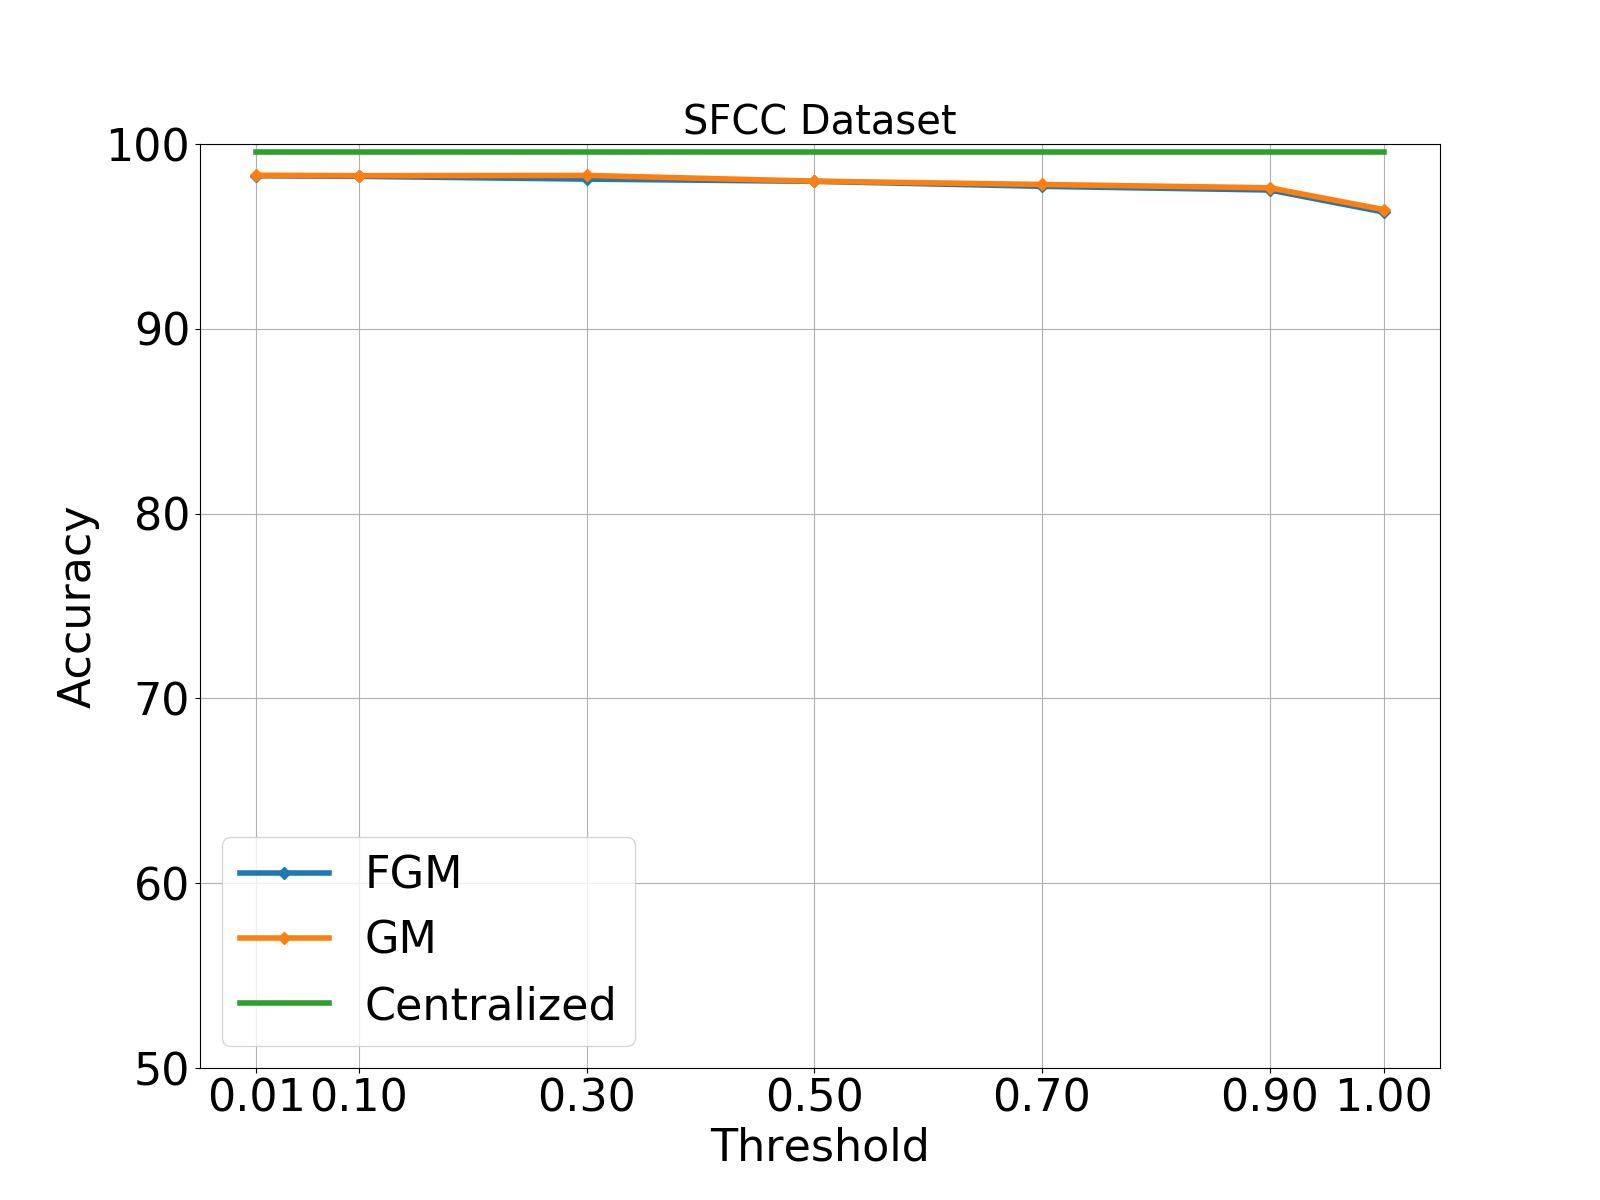
\includegraphics[width=3.9cm,height=3.5cm]{./images/results/sfc-plots/exp_Fig_1_1.png}}
        \subfigure{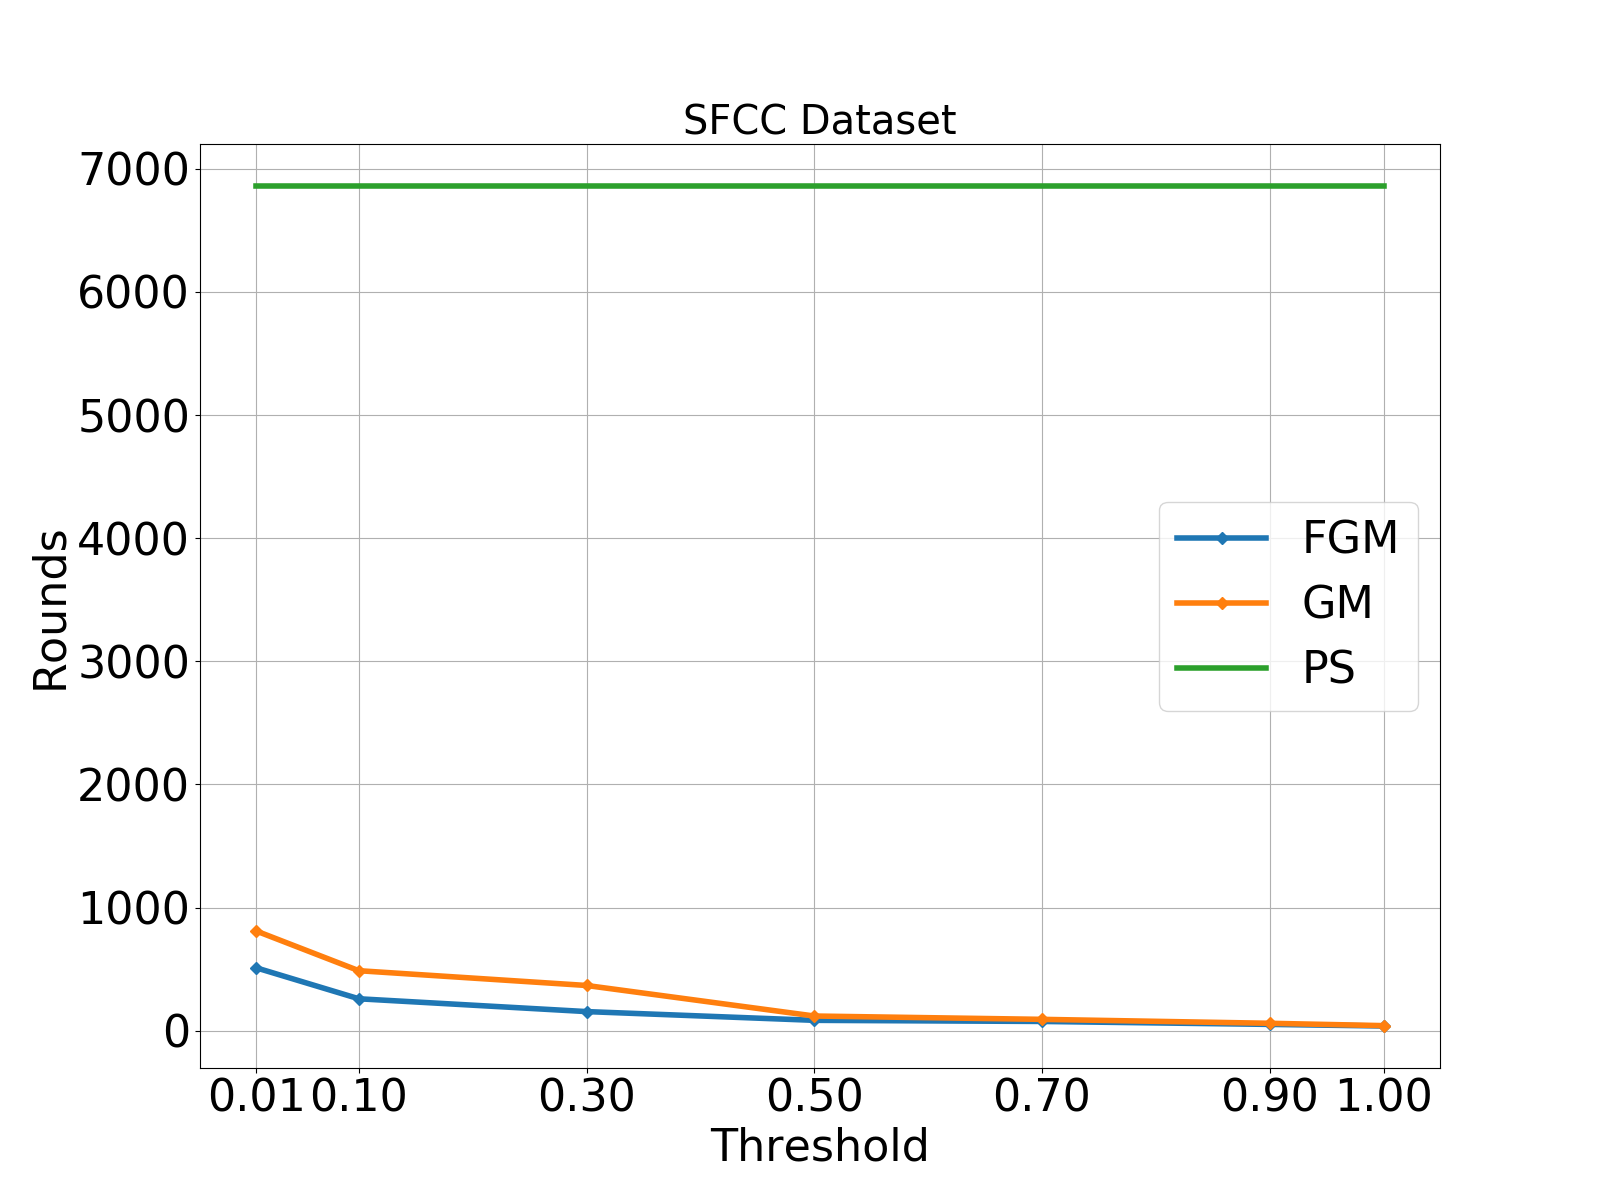
\includegraphics[width=3.9cm,height=3.5cm]{./images/results/sfc-plots/exp_Fig_1_2.png}}
        \subfigure{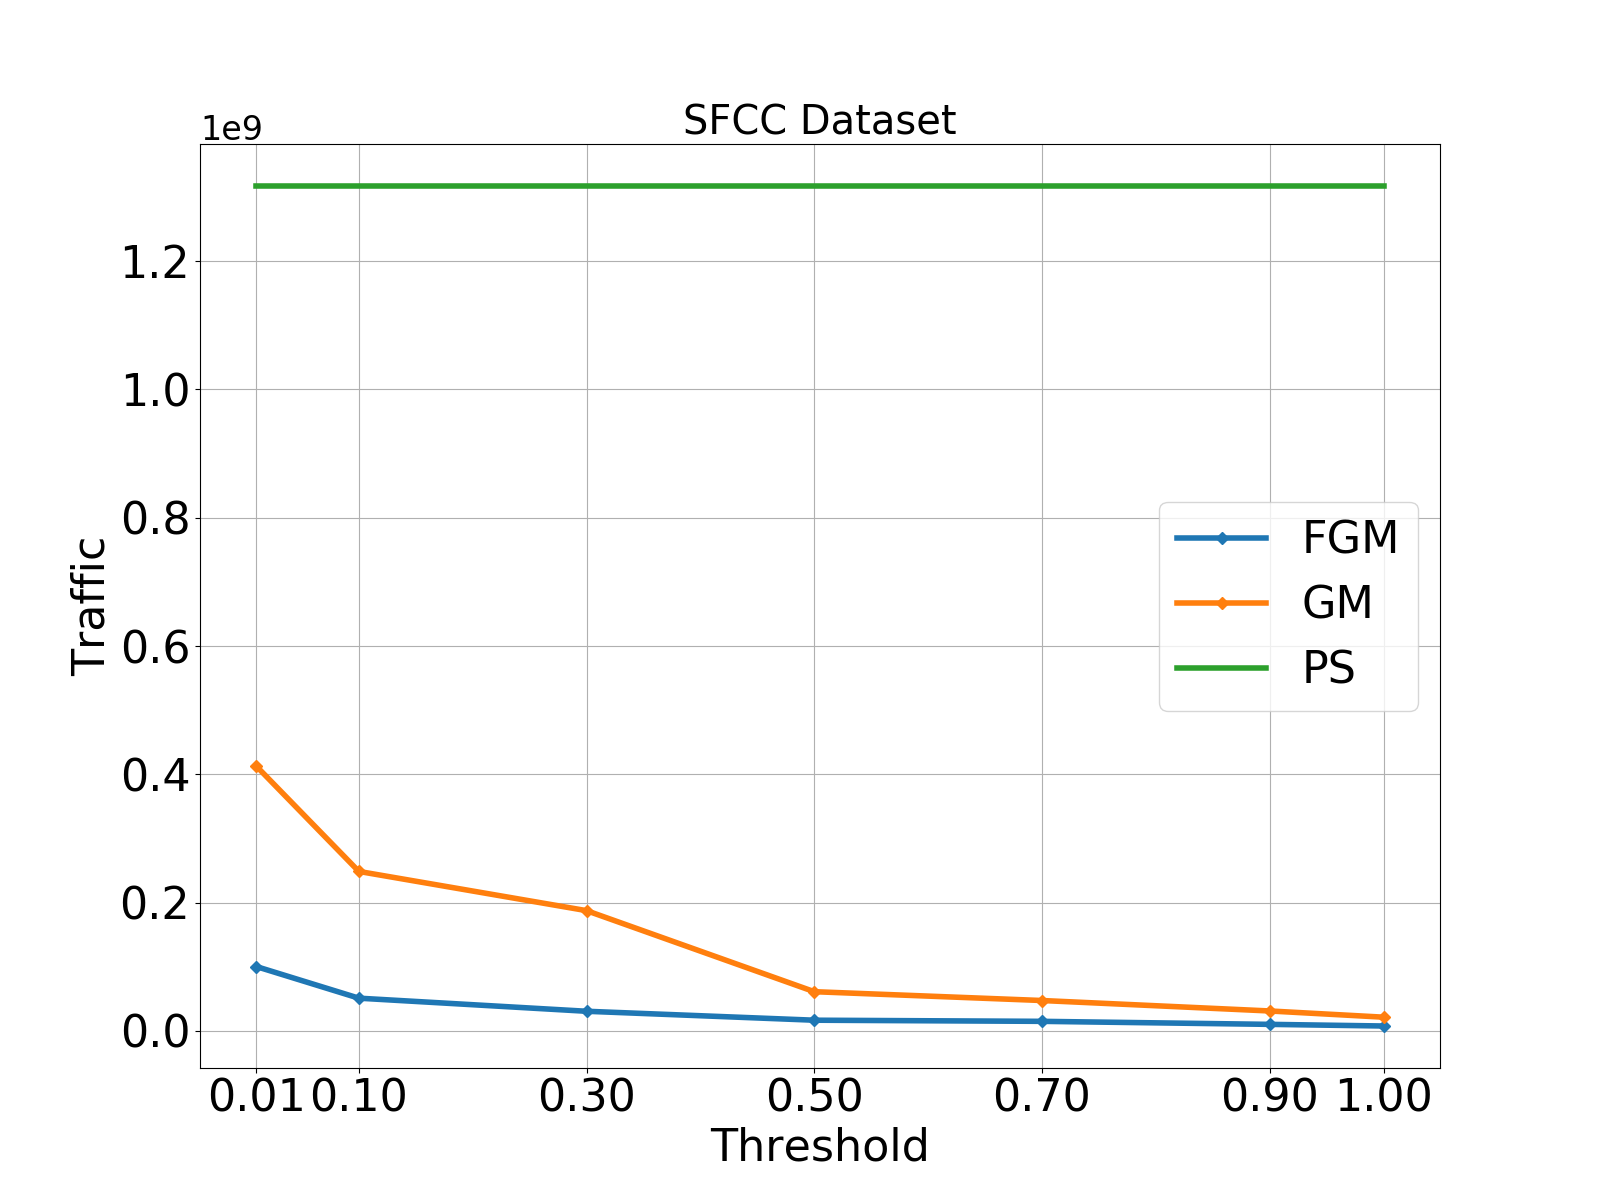
\includegraphics[width=3.9cm,height=3.5cm]{./images/results/sfc-plots/exp_Fig_1_3.png}}
        \subfigure{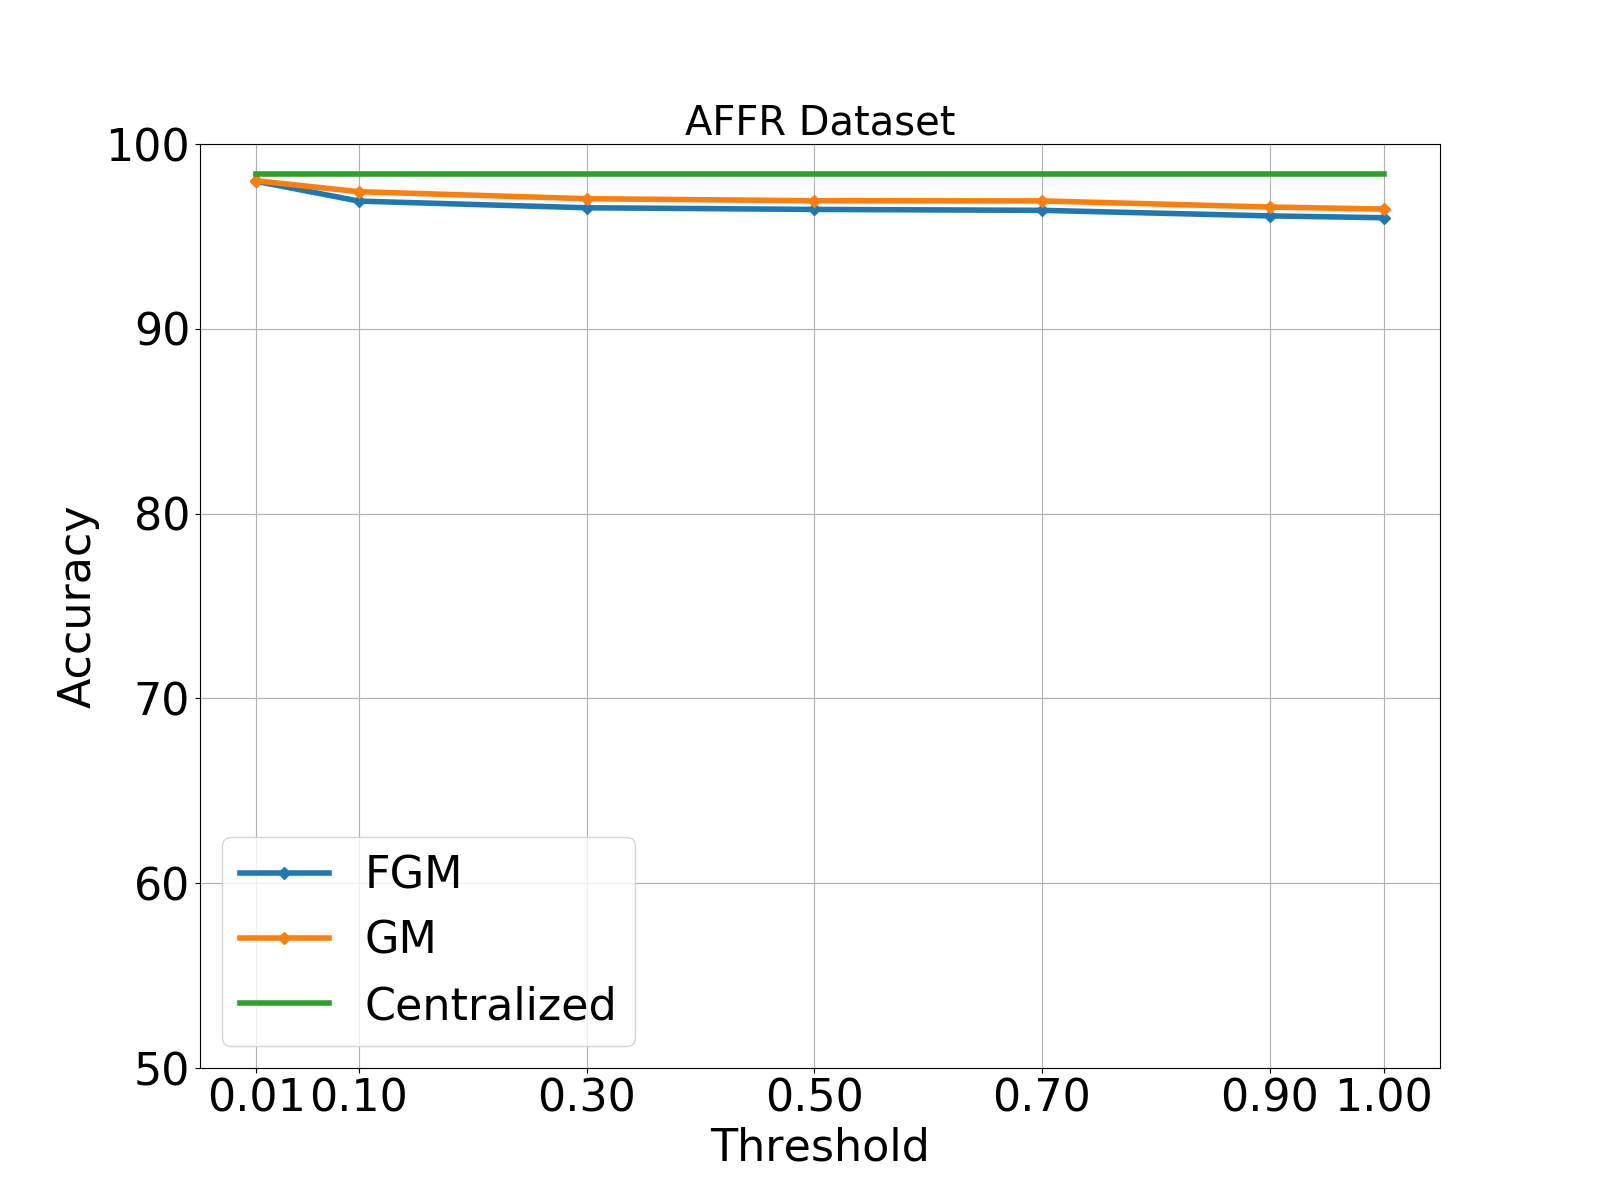
\includegraphics[width=3.9cm,height=3.5cm]{./images/results/amazon-plots/exp_Fig_1_1.png}}
        \subfigure{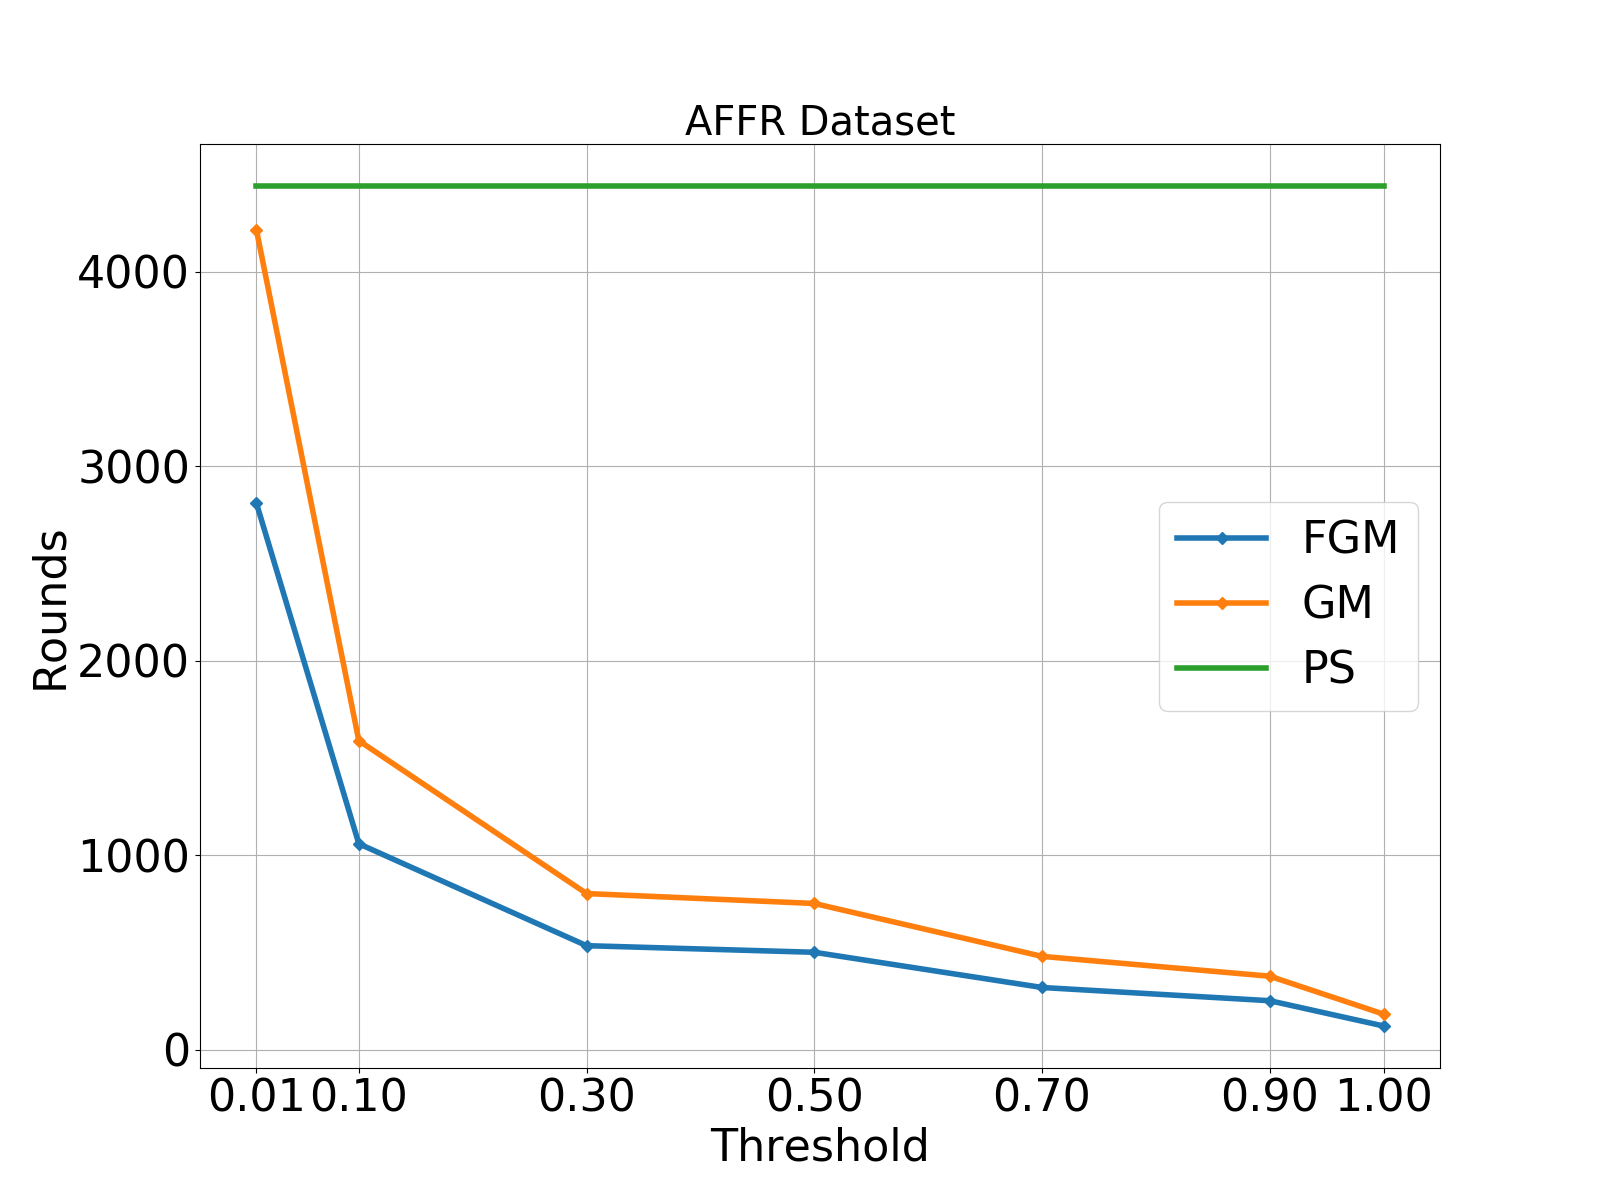
\includegraphics[width=3.9cm,height=3.5cm]{./images/results/amazon-plots/exp_Fig_1_2.png}}
        \subfigure{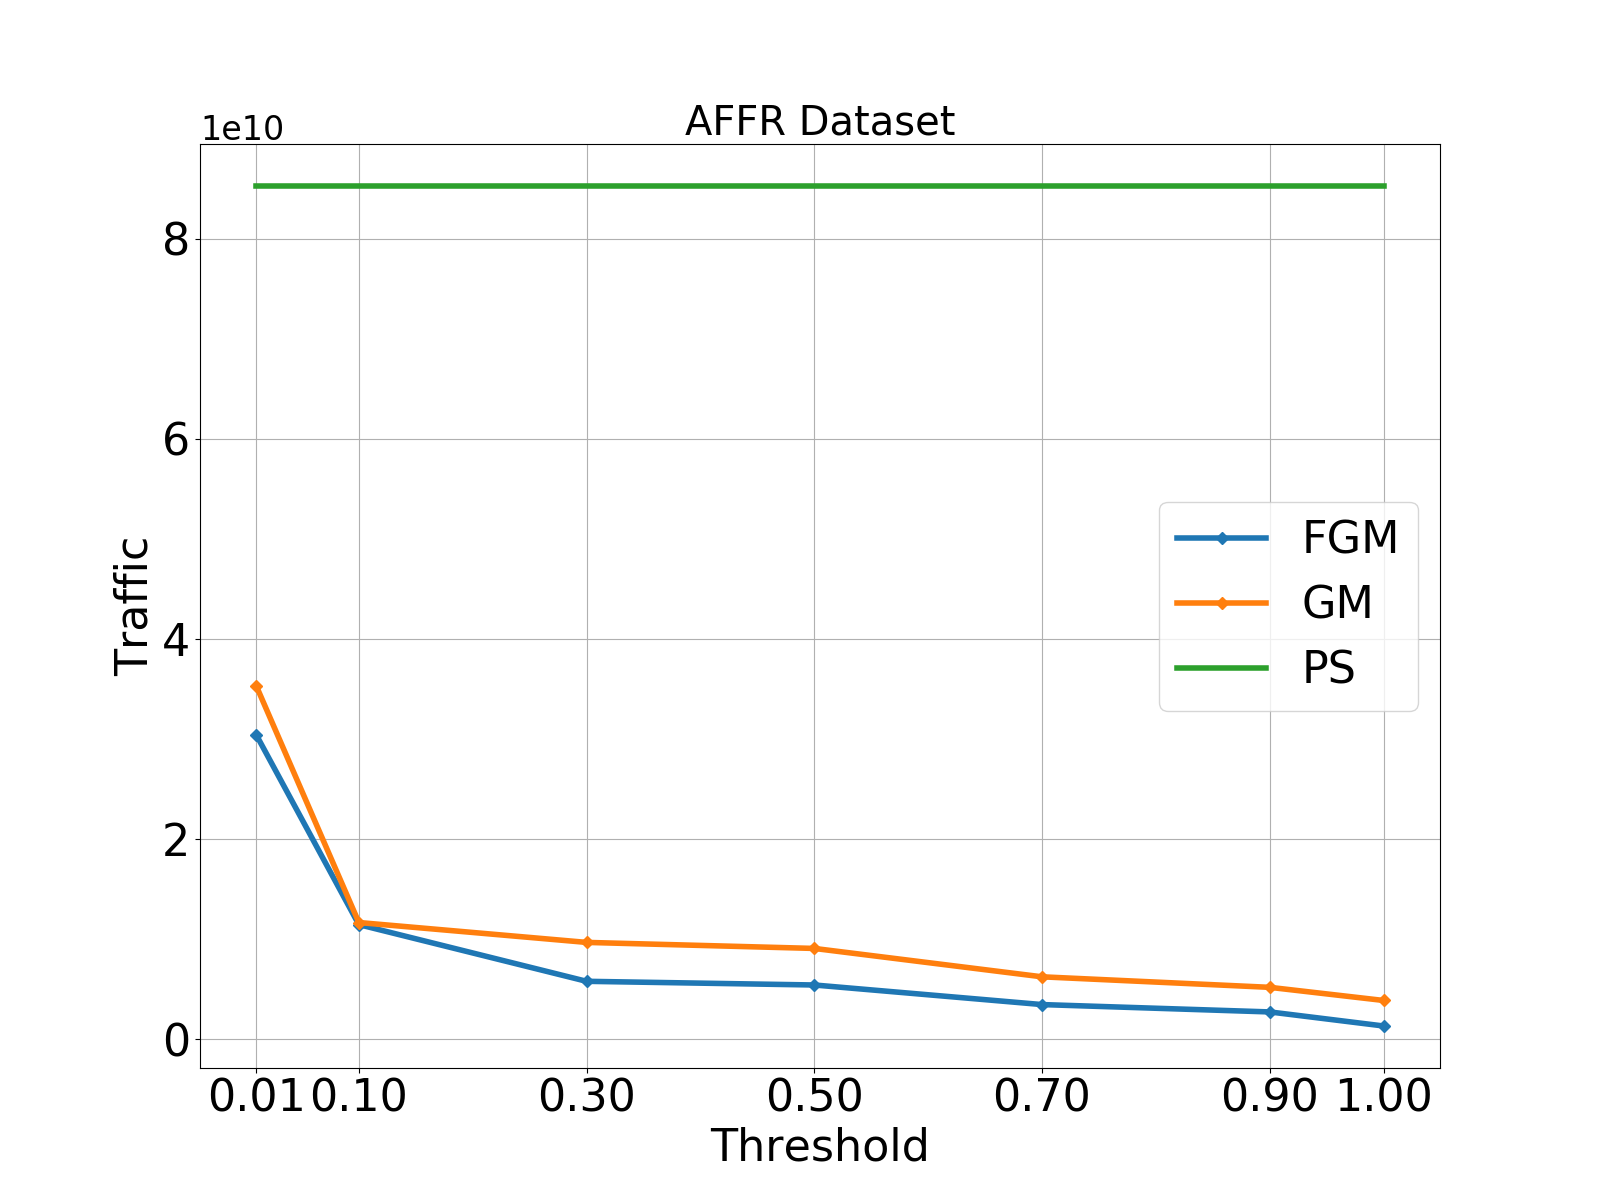
\includegraphics[width=3.9cm,height=3.5cm]{./images/results/amazon-plots/exp_Fig_1_3.png}}
        \label{fig:sfc-amazon-thres}
    \end{figure}
\end{frame}

\begin{frame}{Results (2) - Changing the mini-batch size ($\pmb{|\beta|}$)}
    \begin{itemize}
        \centering
        \item[]{\lbrack threshold=$0.5$, workers=$8$\rbrack}
    \end{itemize}
    \vspace{-0.3cm}
    \begin{figure}
        \subfigure{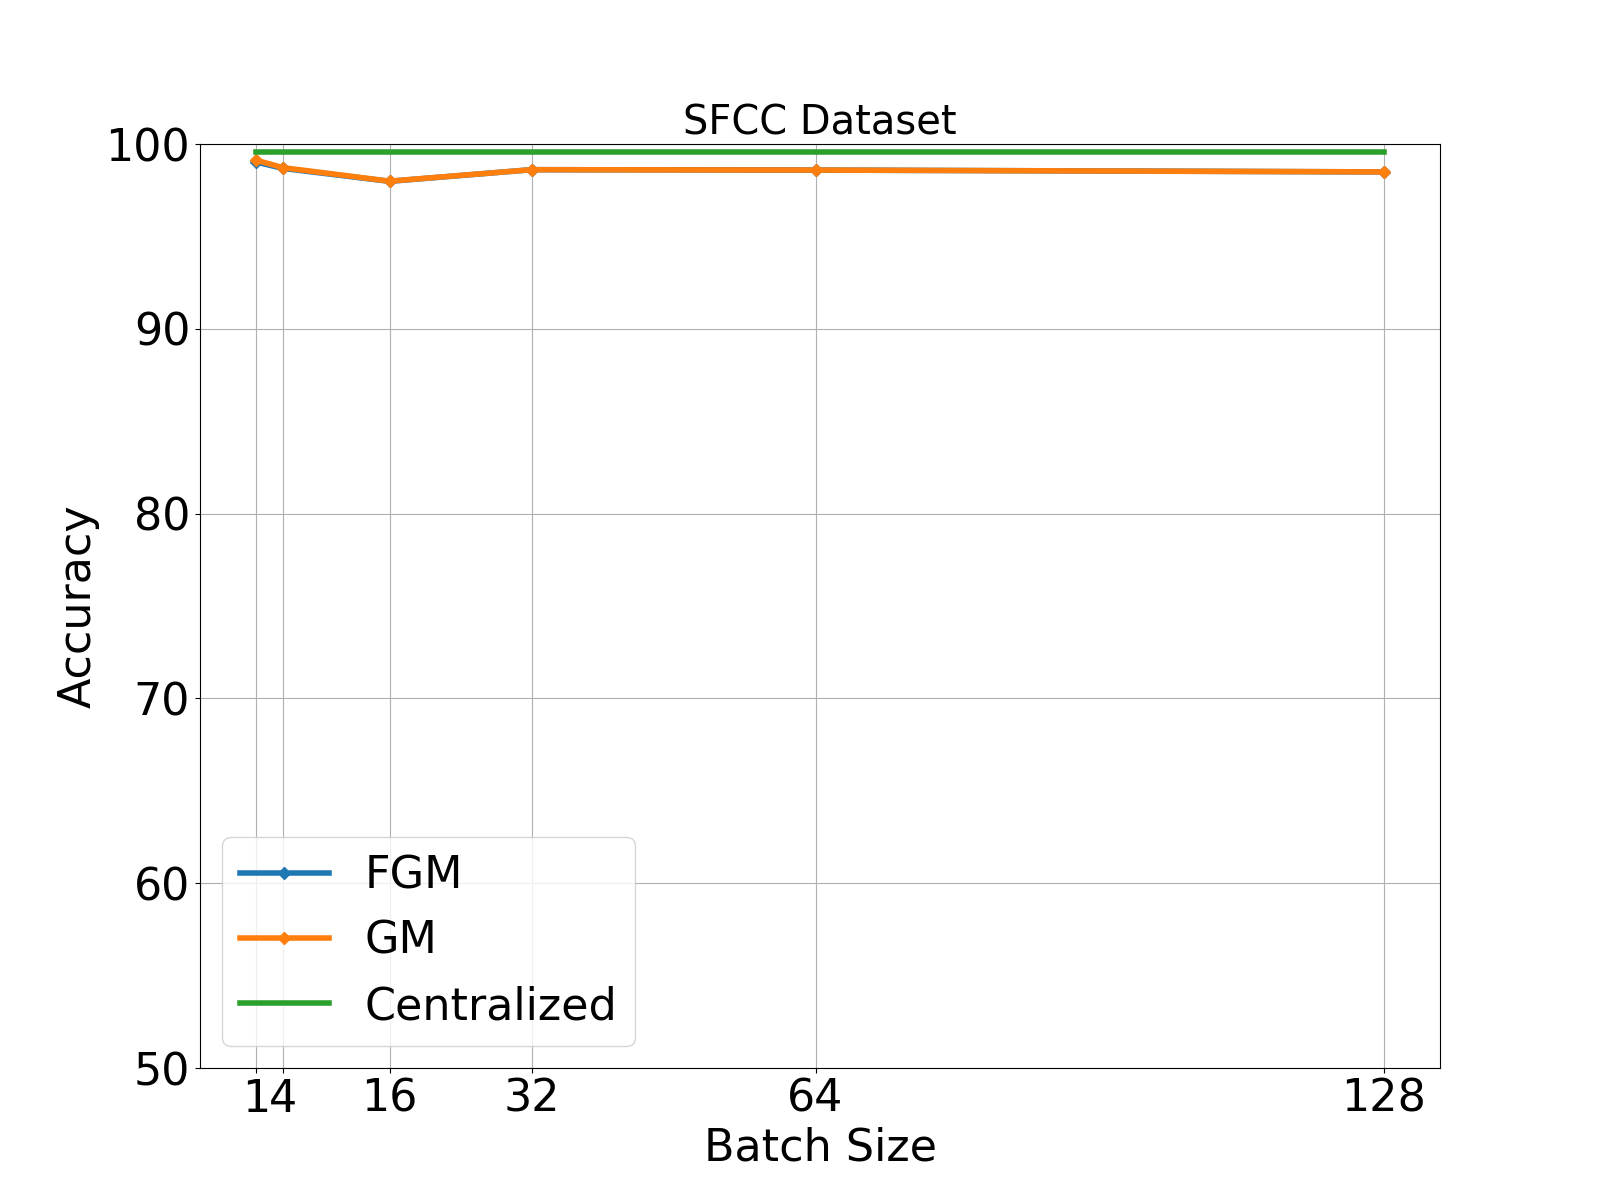
\includegraphics[width=3.9cm,height=3.5cm]{./images/results/sfc-plots/exp_Fig_2_1.png}}
        \subfigure{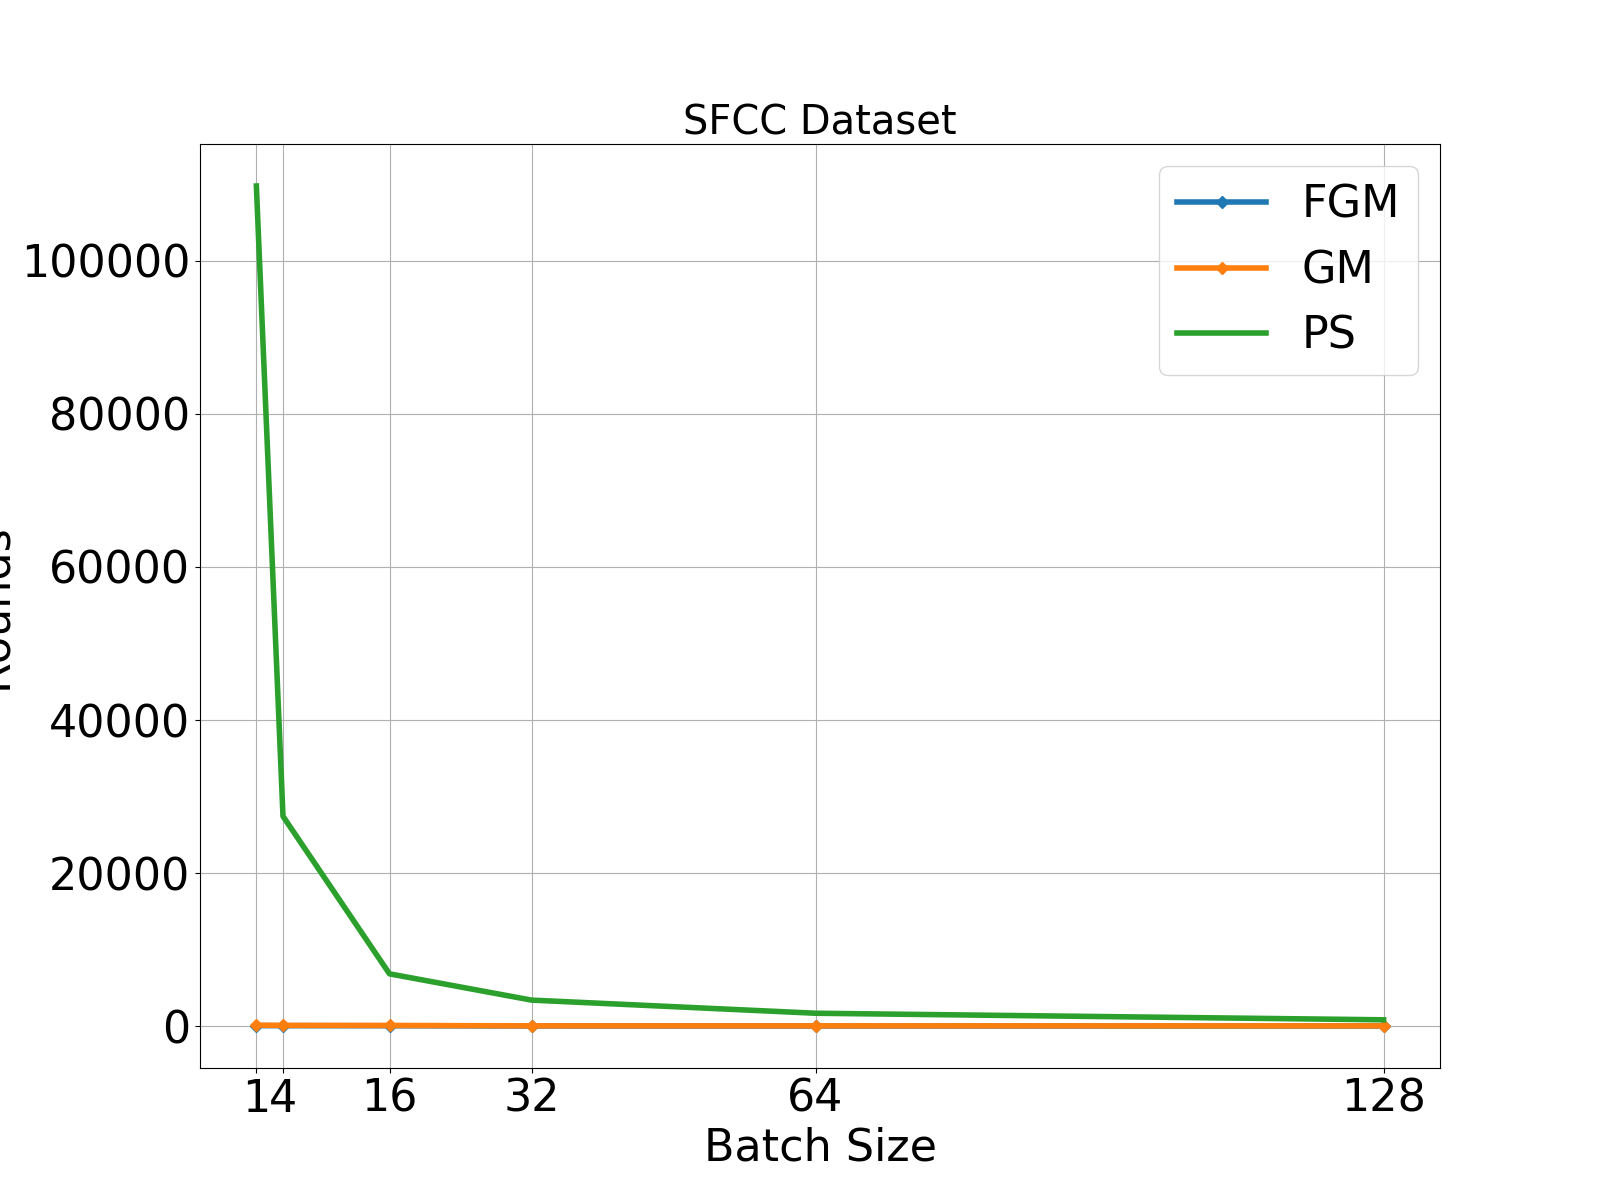
\includegraphics[width=3.9cm,height=3.5cm]{./images/results/sfc-plots/exp_Fig_2_2.png}}
        \subfigure{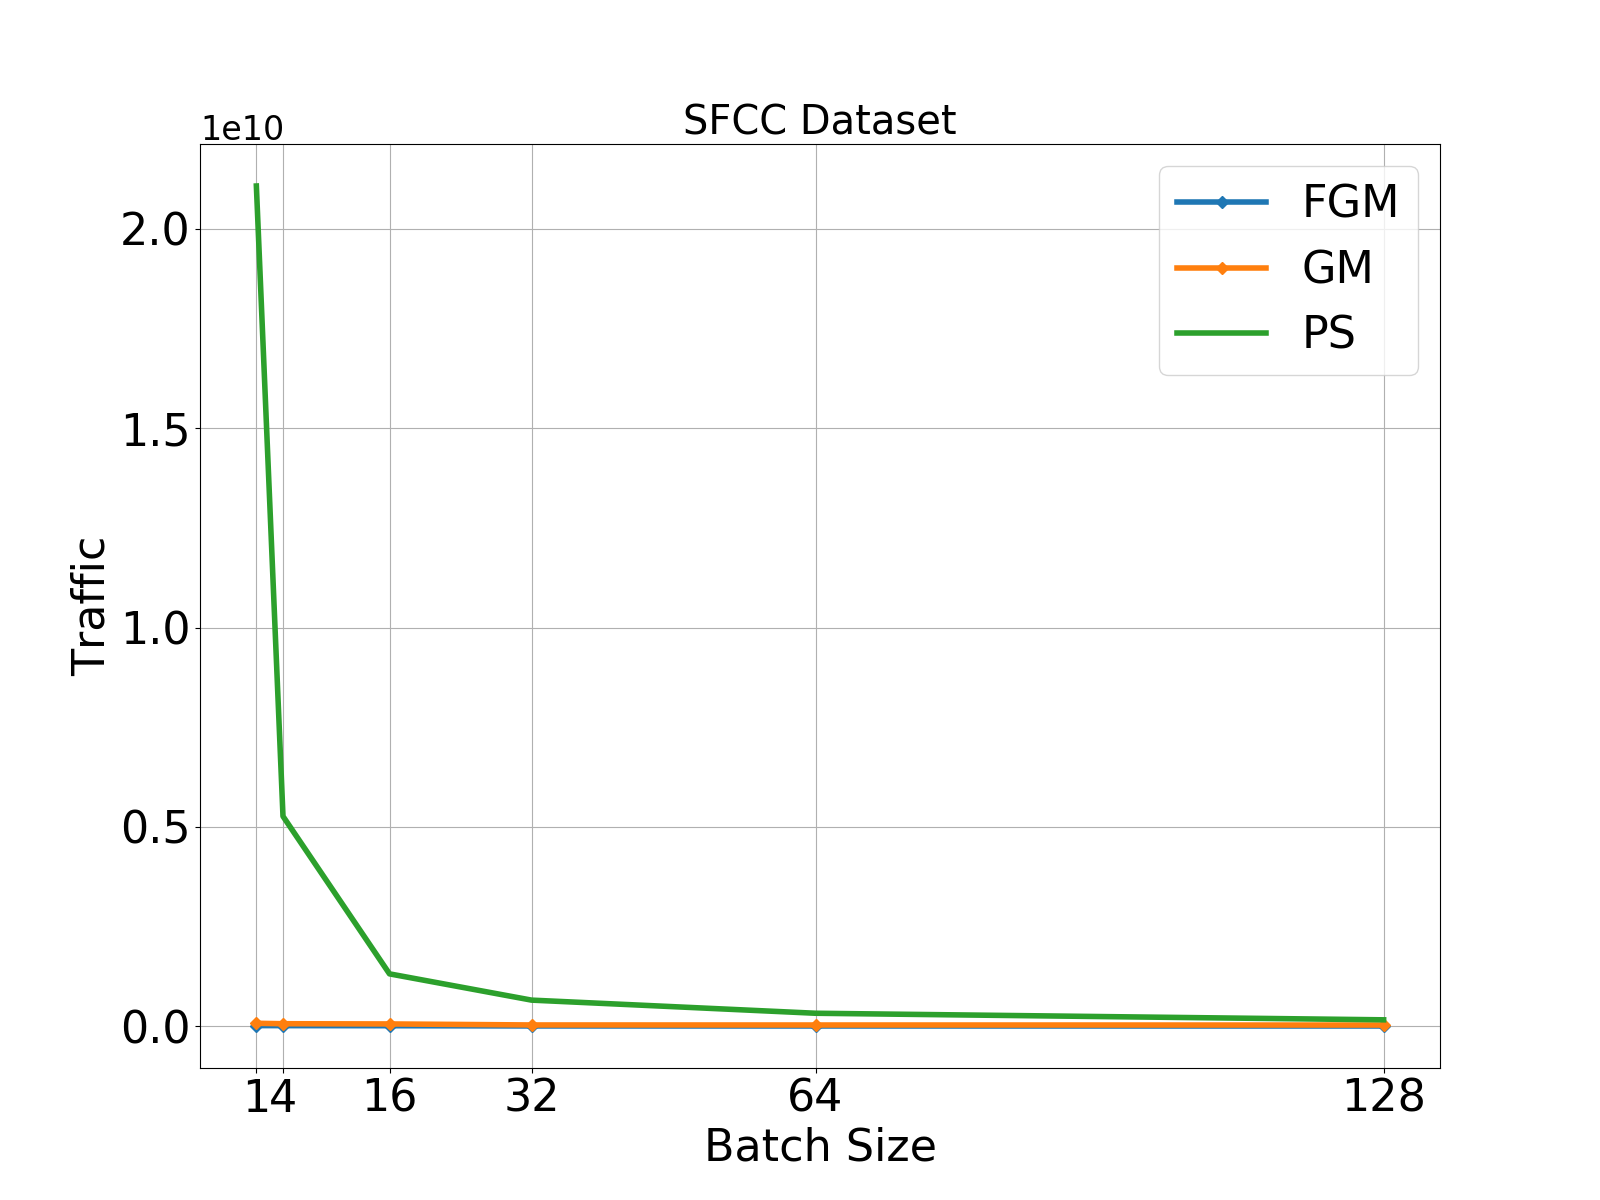
\includegraphics[width=3.9cm,height=3.5cm]{./images/results/sfc-plots/exp_Fig_2_3.png}}
        \subfigure{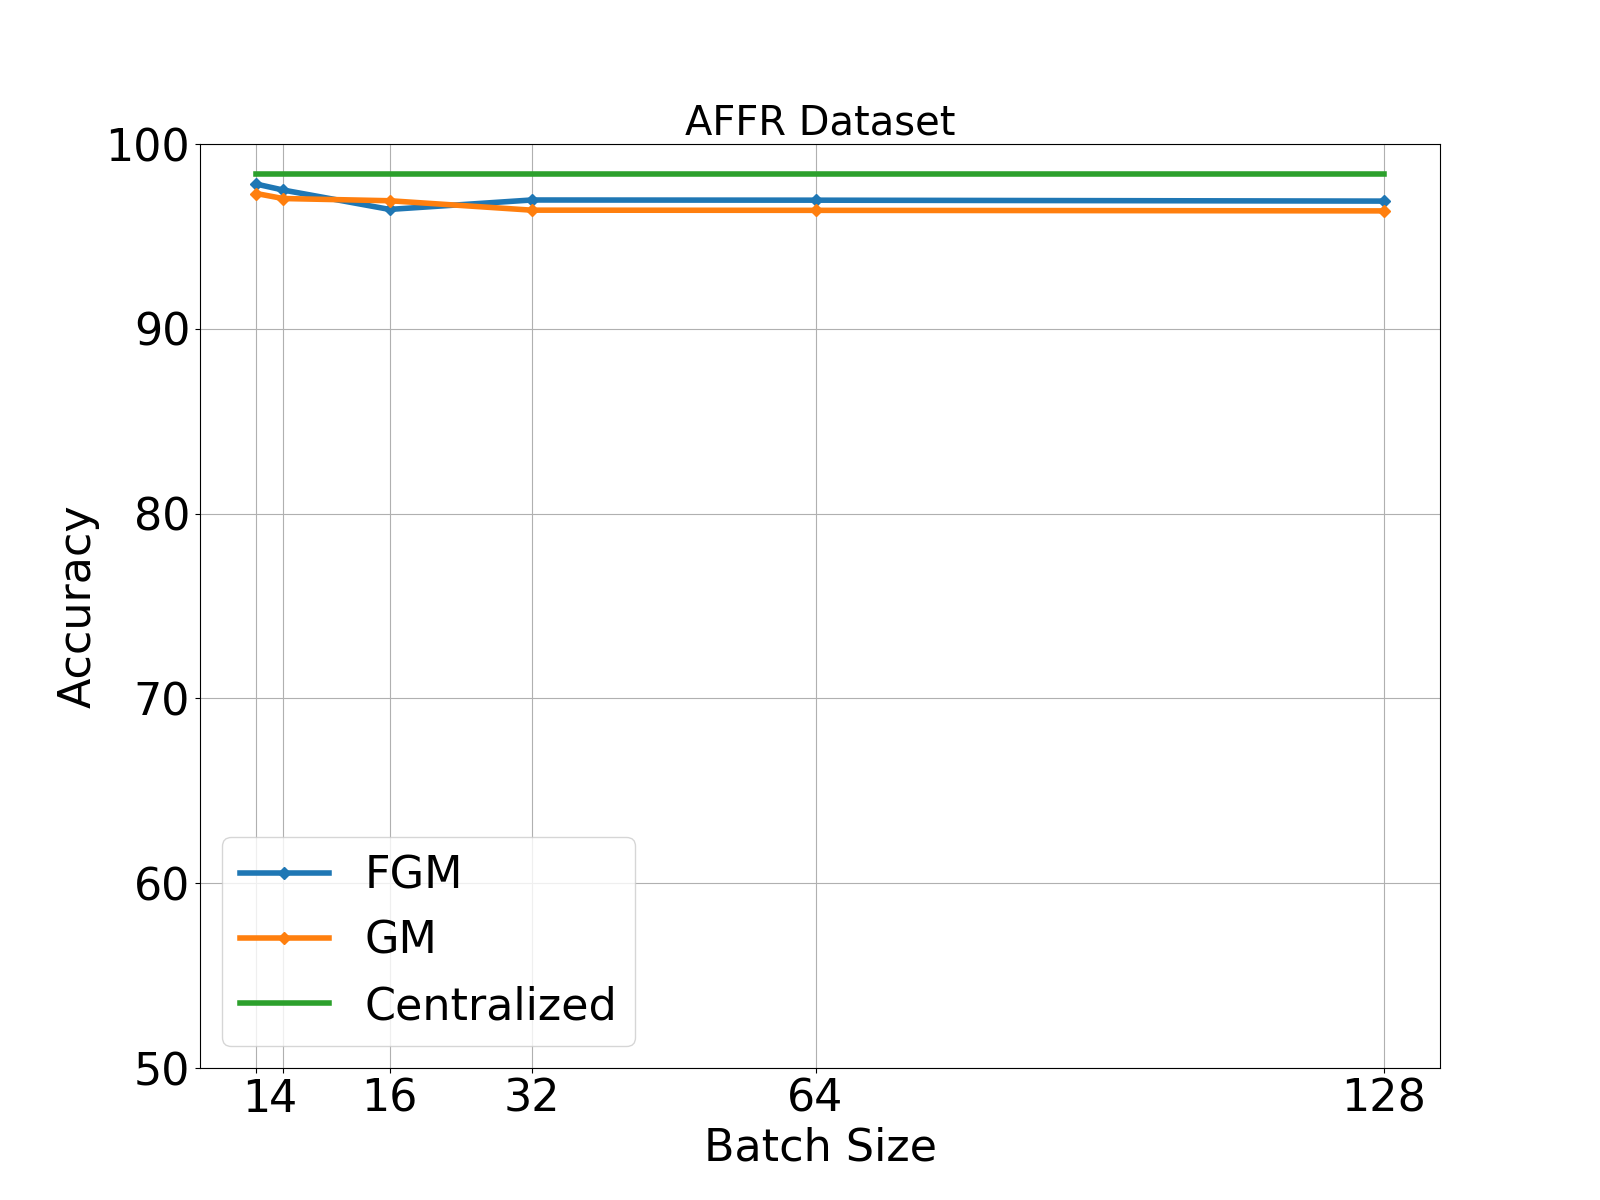
\includegraphics[width=3.9cm,height=3.5cm]{./images/results/amazon-plots/exp_Fig_2_1.png}}
        \subfigure{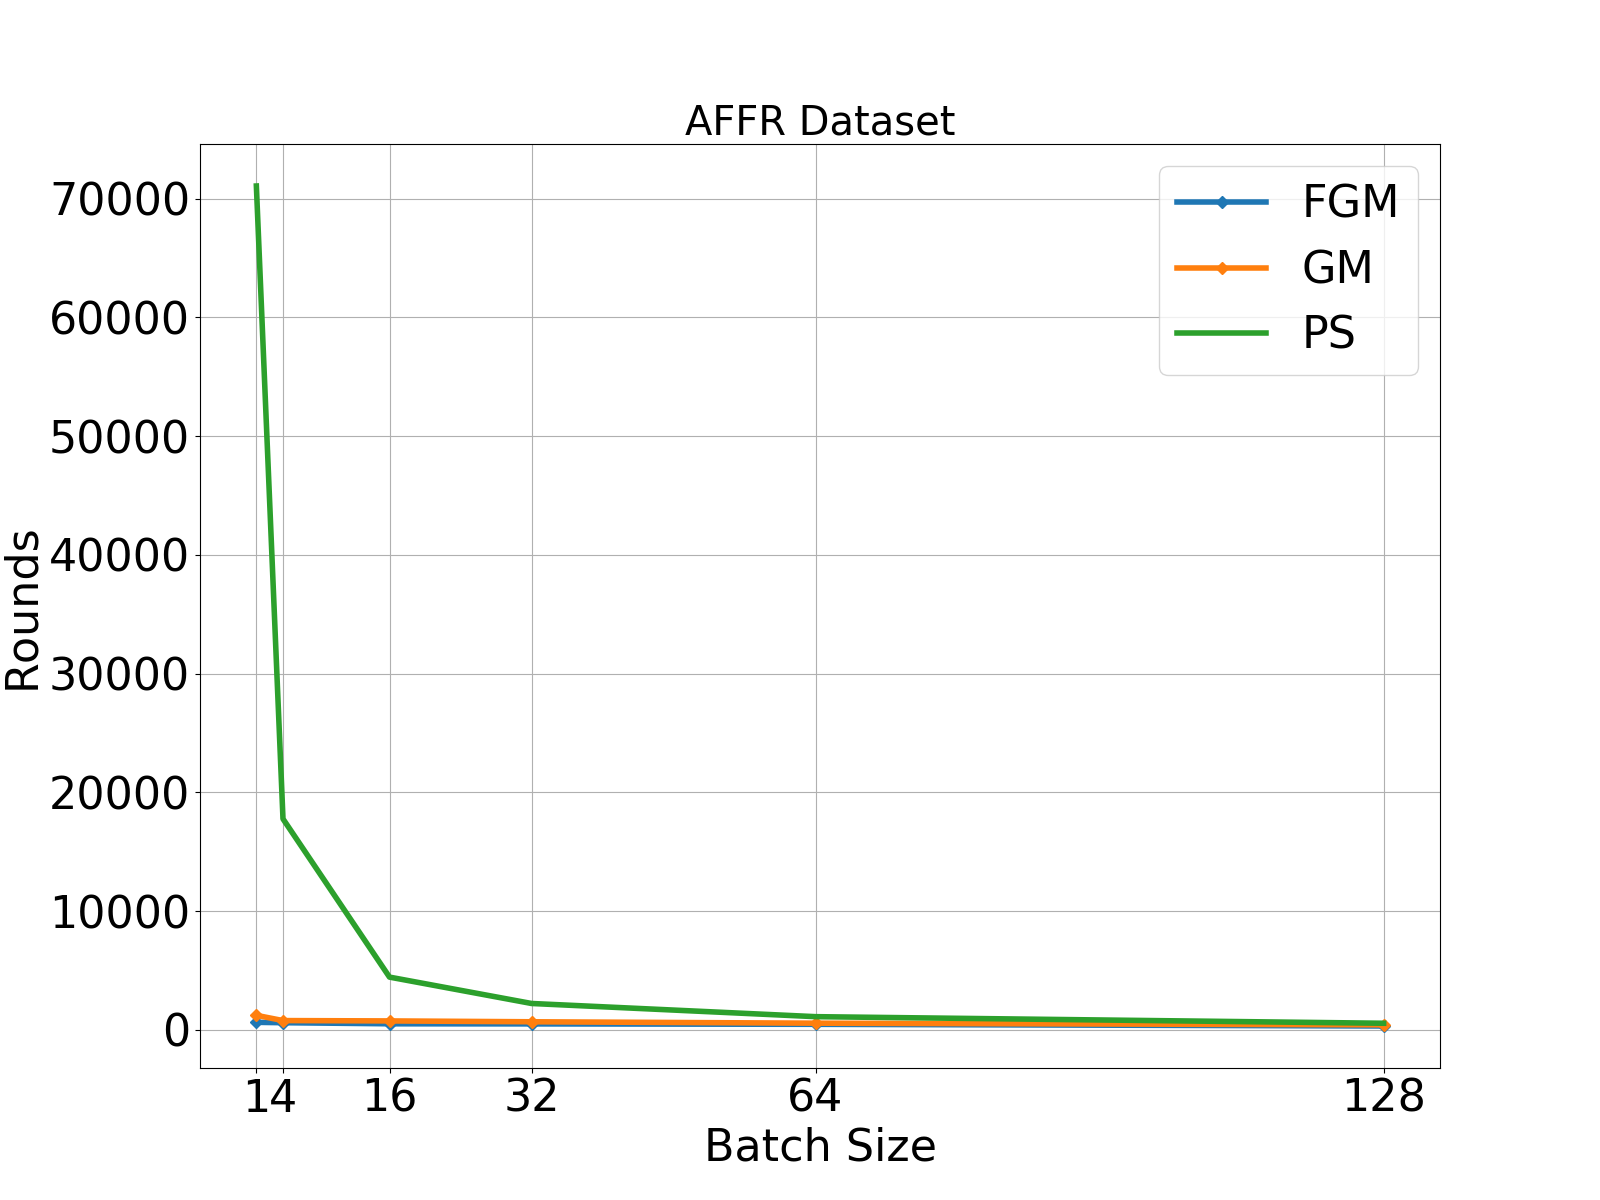
\includegraphics[width=3.9cm,height=3.5cm]{./images/results/amazon-plots/exp_Fig_2_2.png}}
        \subfigure{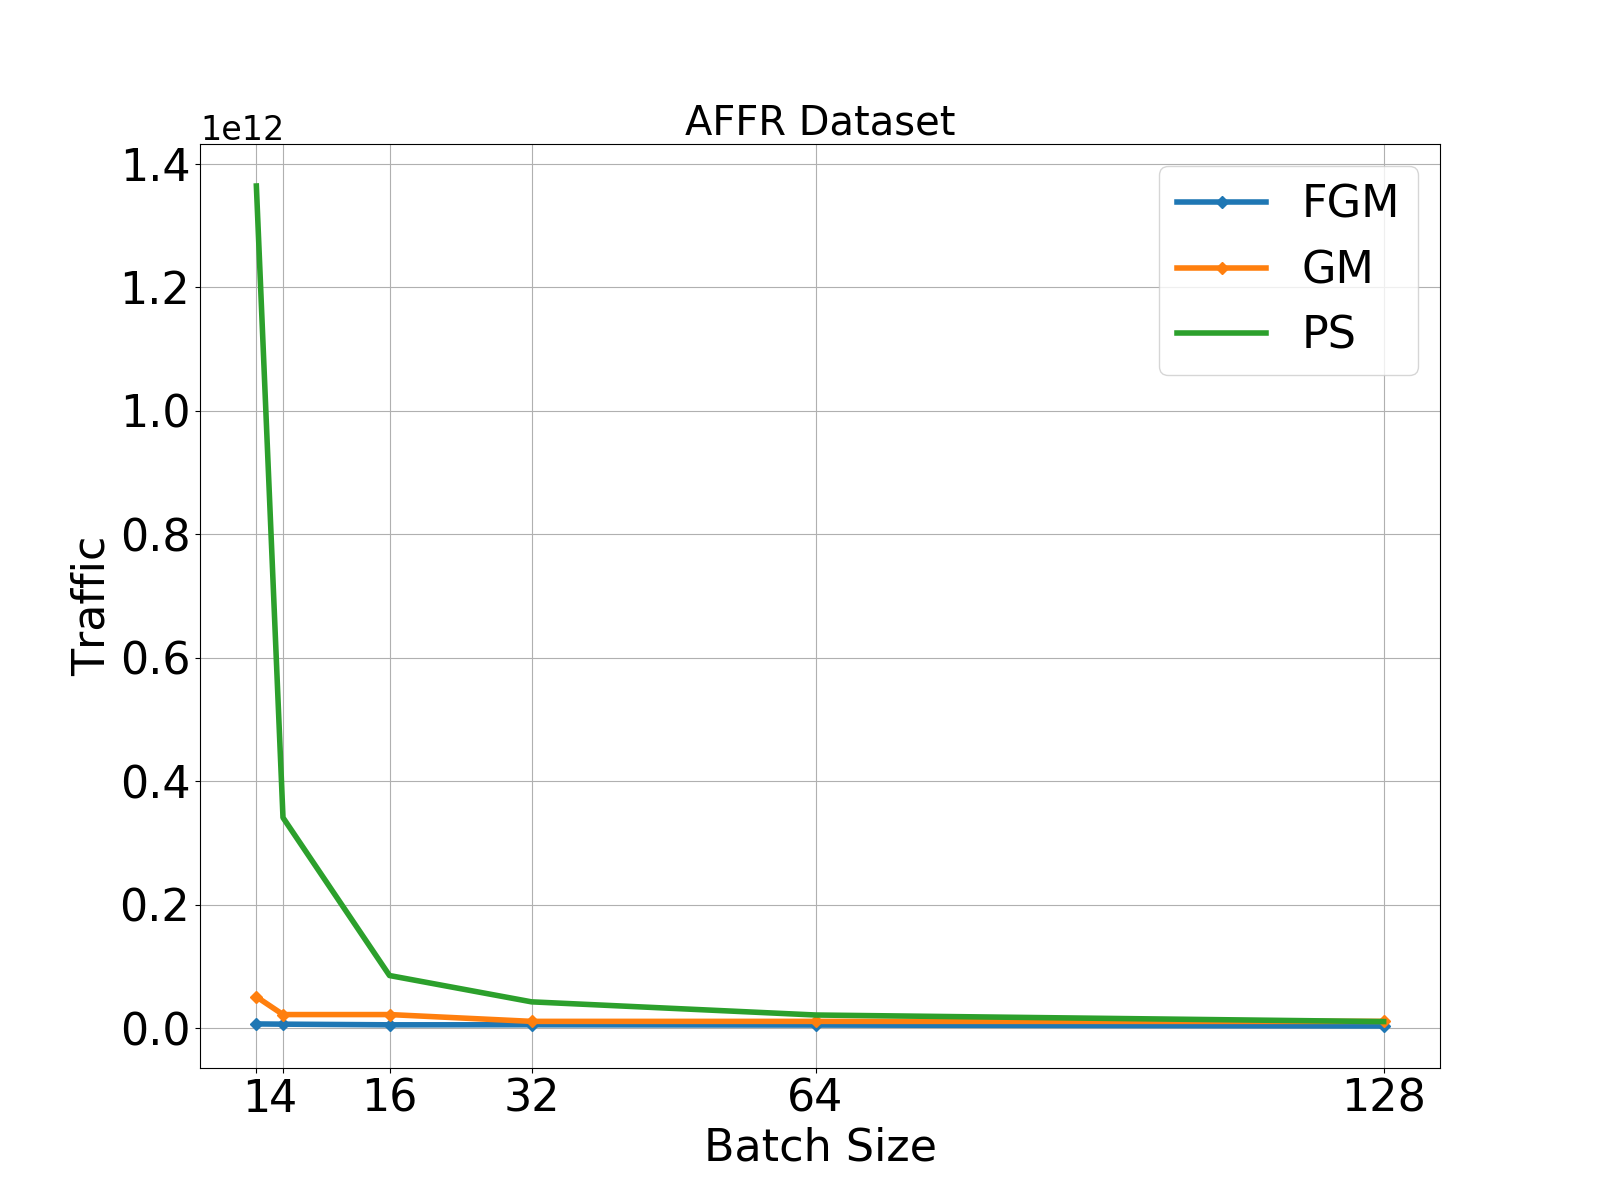
\includegraphics[width=3.9cm,height=3.5cm]{./images/results/amazon-plots/exp_Fig_2_3.png}}
        \label{fig:sfc-amazon-bs}
    \end{figure}
\end{frame}

\begin{frame}{Results (3) - Changing the number of workers ($\pmb{n}$)}
    \begin{itemize}
        \centering
        \item[]{\lbrack threshold=$0.5$, mini-batch=$16$\rbrack}
    \end{itemize}
    \vspace{-0.3cm}
    \begin{figure}
        \subfigure{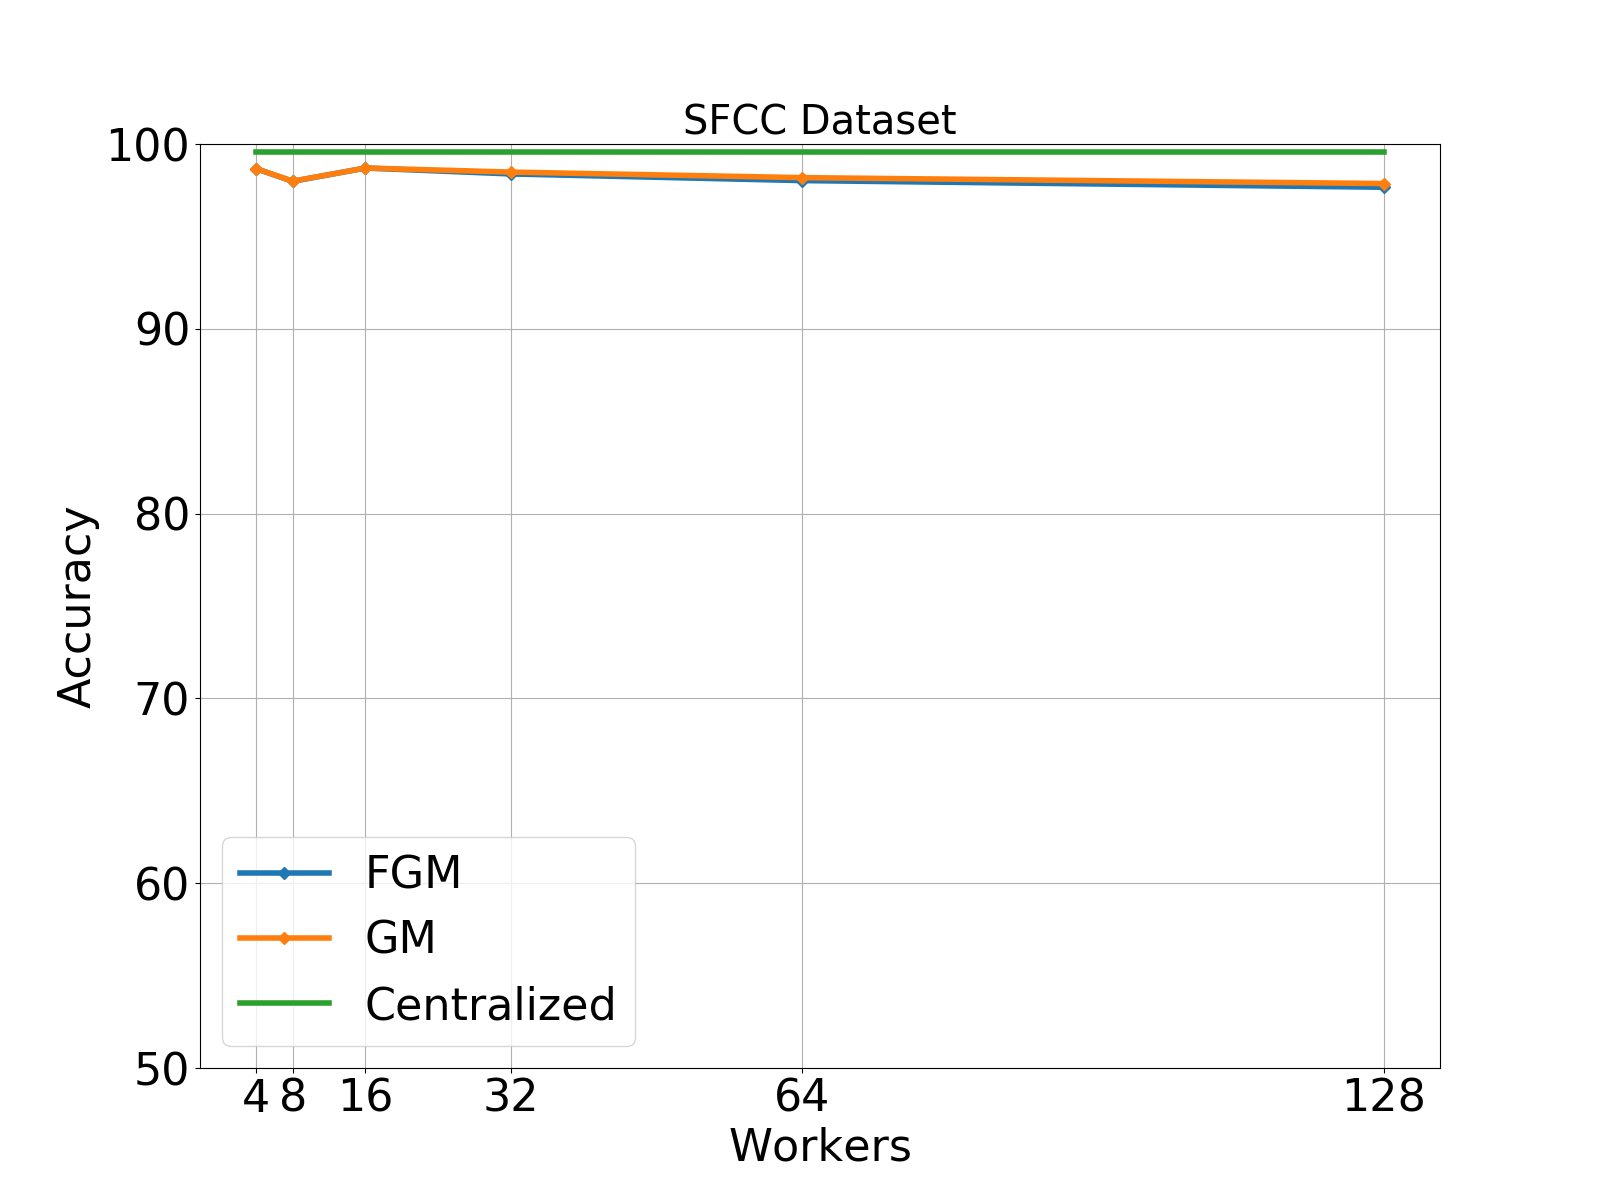
\includegraphics[width=3.9cm,height=3.5cm]{./images/results/sfc-plots/exp_Fig_3_1.png}}
        \subfigure{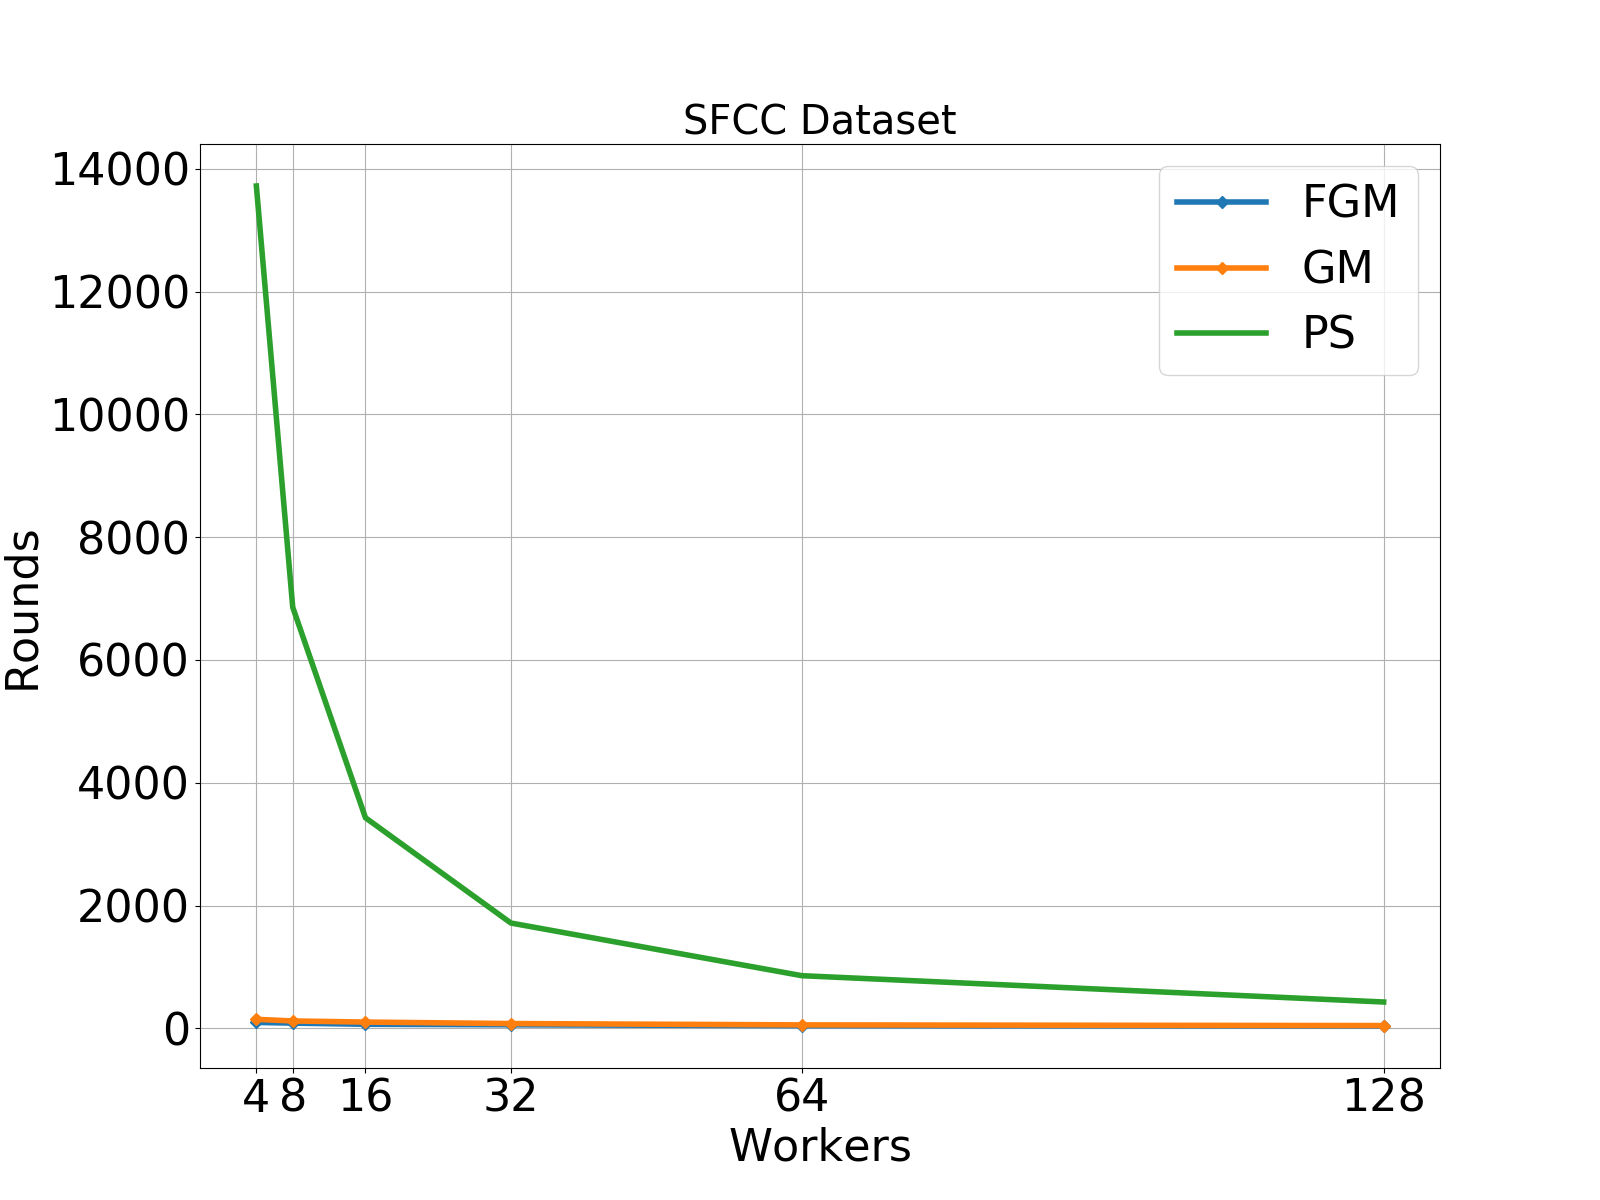
\includegraphics[width=3.9cm,height=3.5cm]{./images/results/sfc-plots/exp_Fig_3_2.png}}
        \subfigure{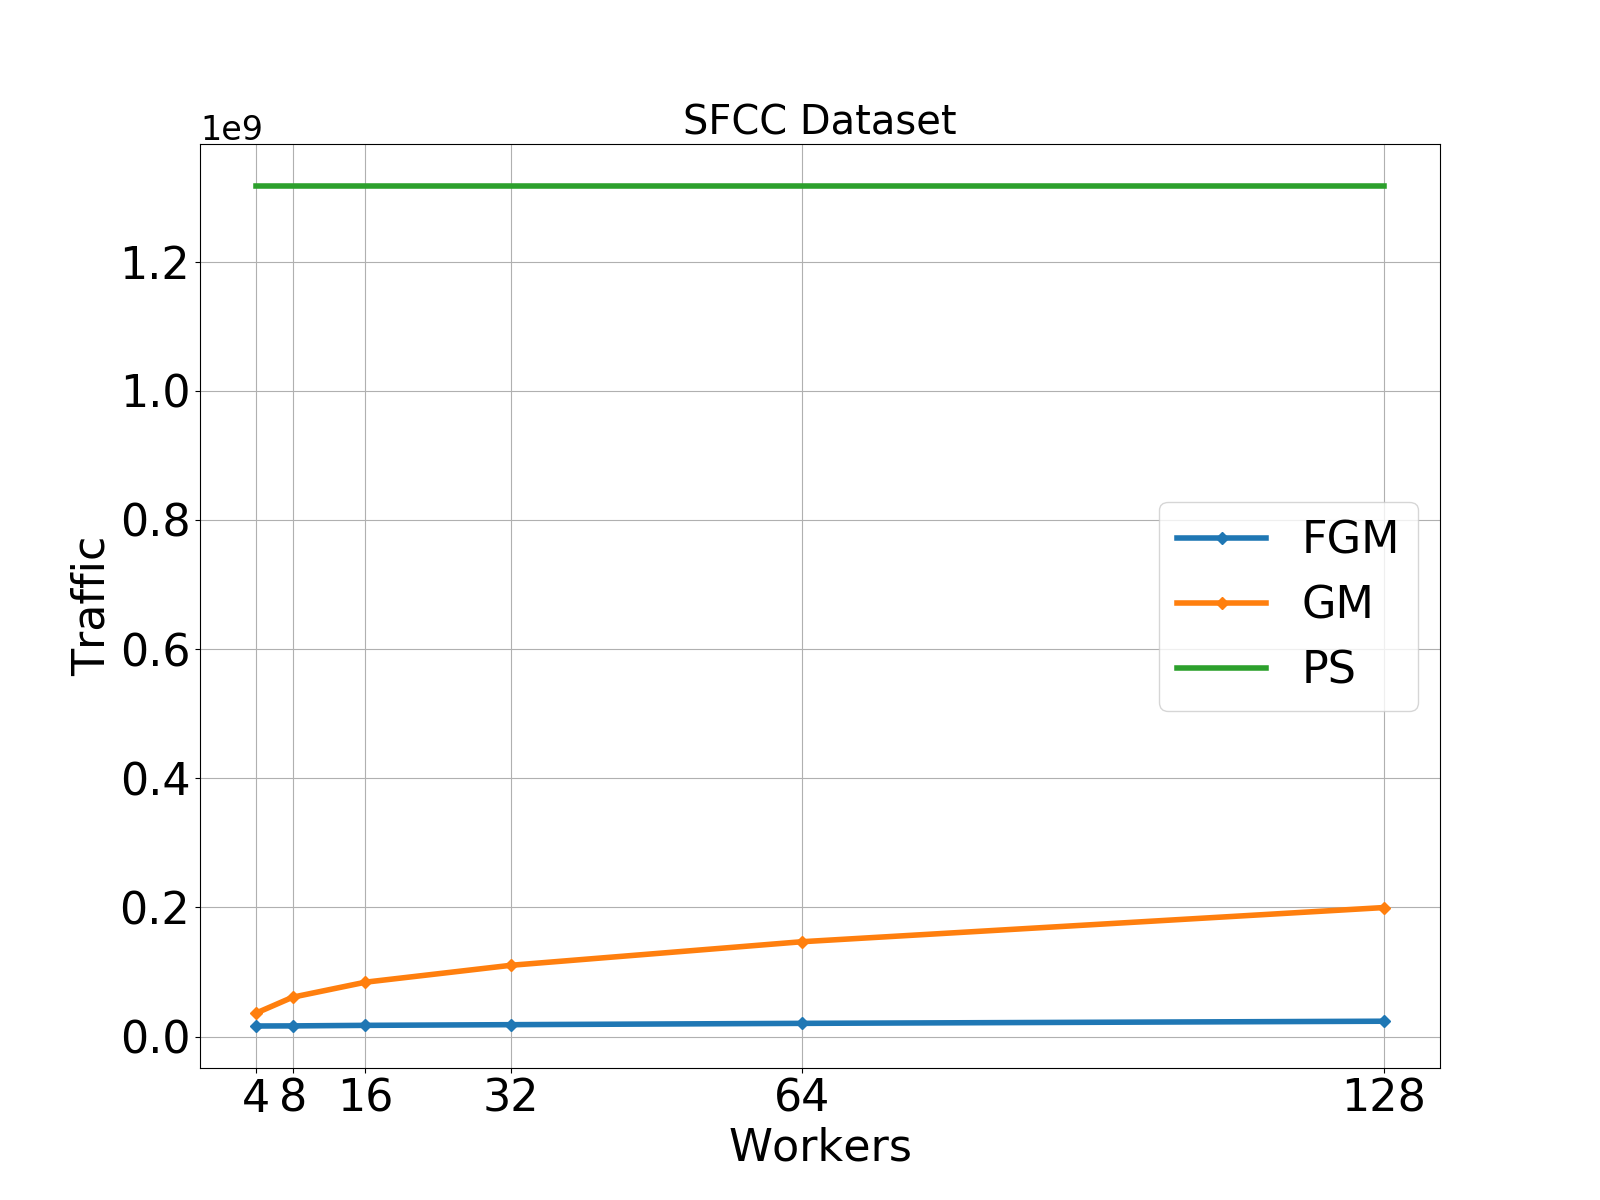
\includegraphics[width=3.9cm,height=3.5cm]{./images/results/sfc-plots/exp_Fig_3_3.png}}
        \subfigure{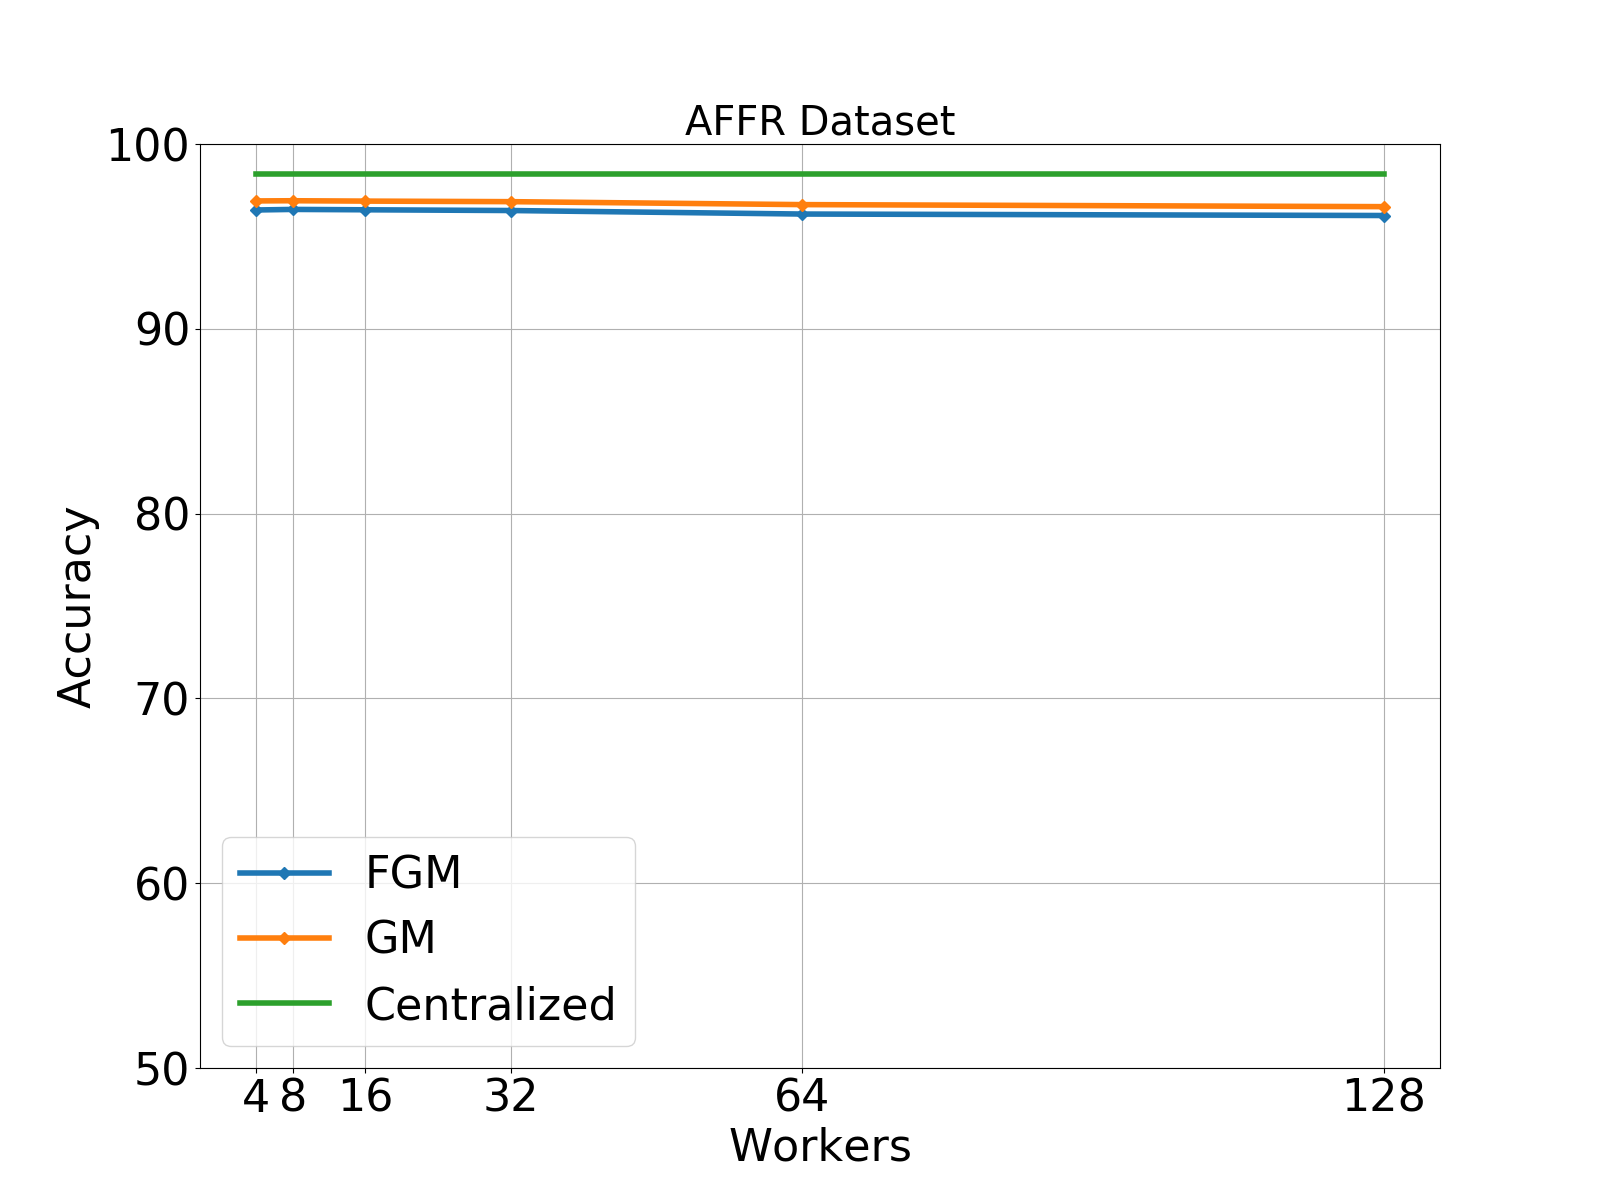
\includegraphics[width=3.9cm,height=3.5cm]{./images/results/amazon-plots/exp_Fig_3_1.png}}
        \subfigure{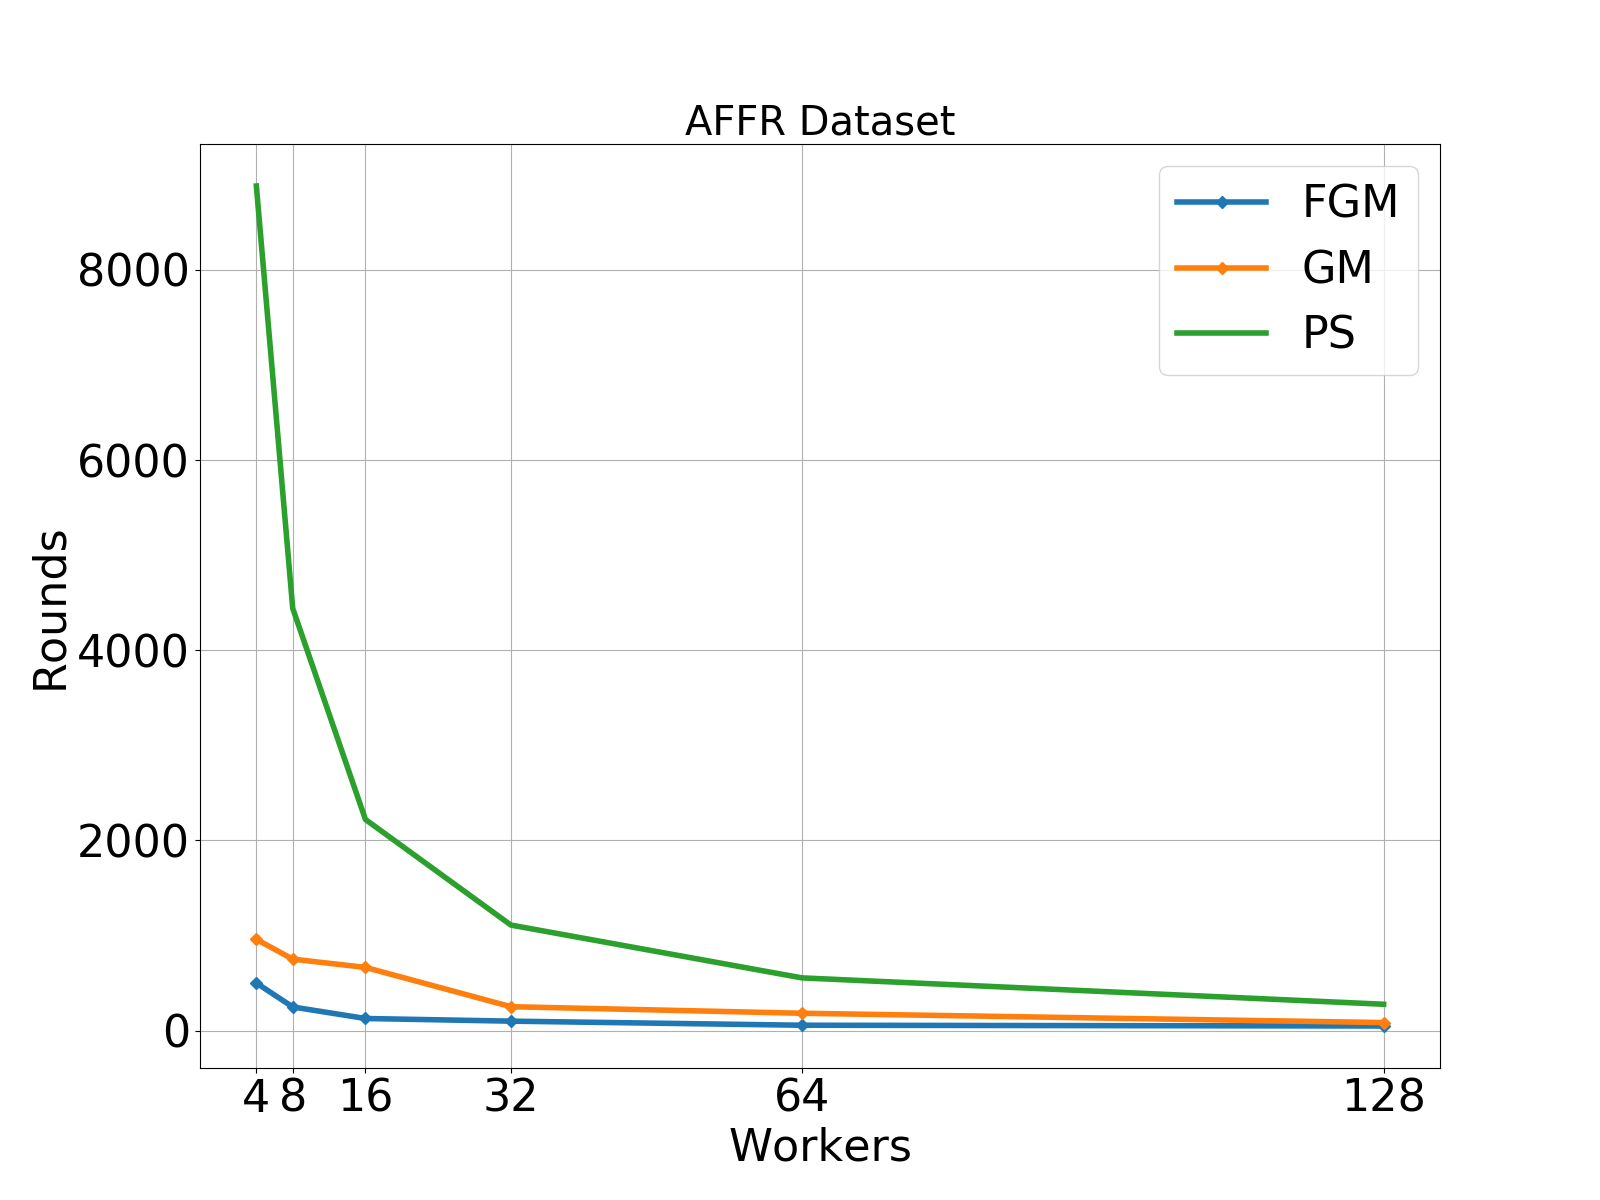
\includegraphics[width=3.9cm,height=3.5cm]{./images/results/amazon-plots/exp_Fig_3_2.png}}
        \subfigure{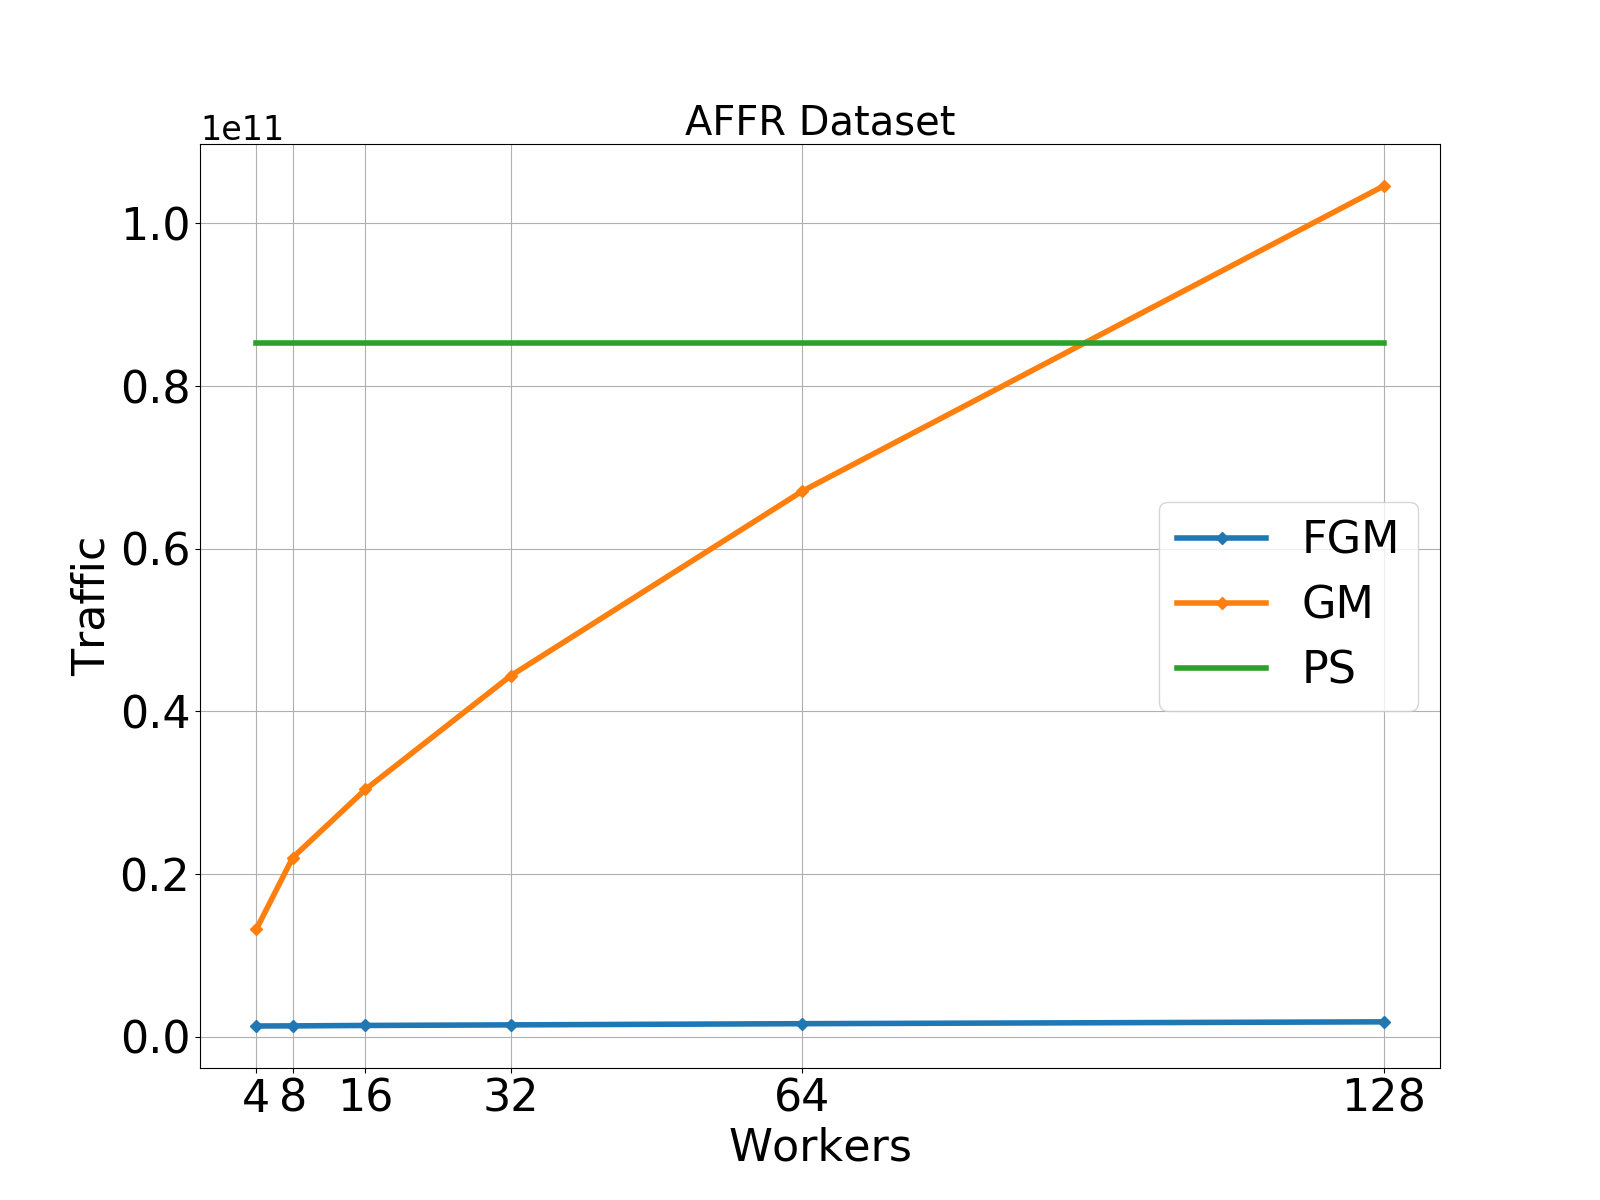
\includegraphics[width=3.9cm,height=3.5cm]{./images/results/amazon-plots/exp_Fig_3_3.png}}
        \label{fig:sfc-amazon-workers}
    \end{figure}
\end{frame}

\begin{frame}{Results (4) - Focusing on a specific case}
    \begin{itemize}
        \centering
        \item[]{\lbrack threshold=$\{0.1, 0.5\}$, mini-batch=$16$\rbrack}
    \end{itemize}
    \vspace{-0.3cm}
    \begin{figure}
        \subfigure{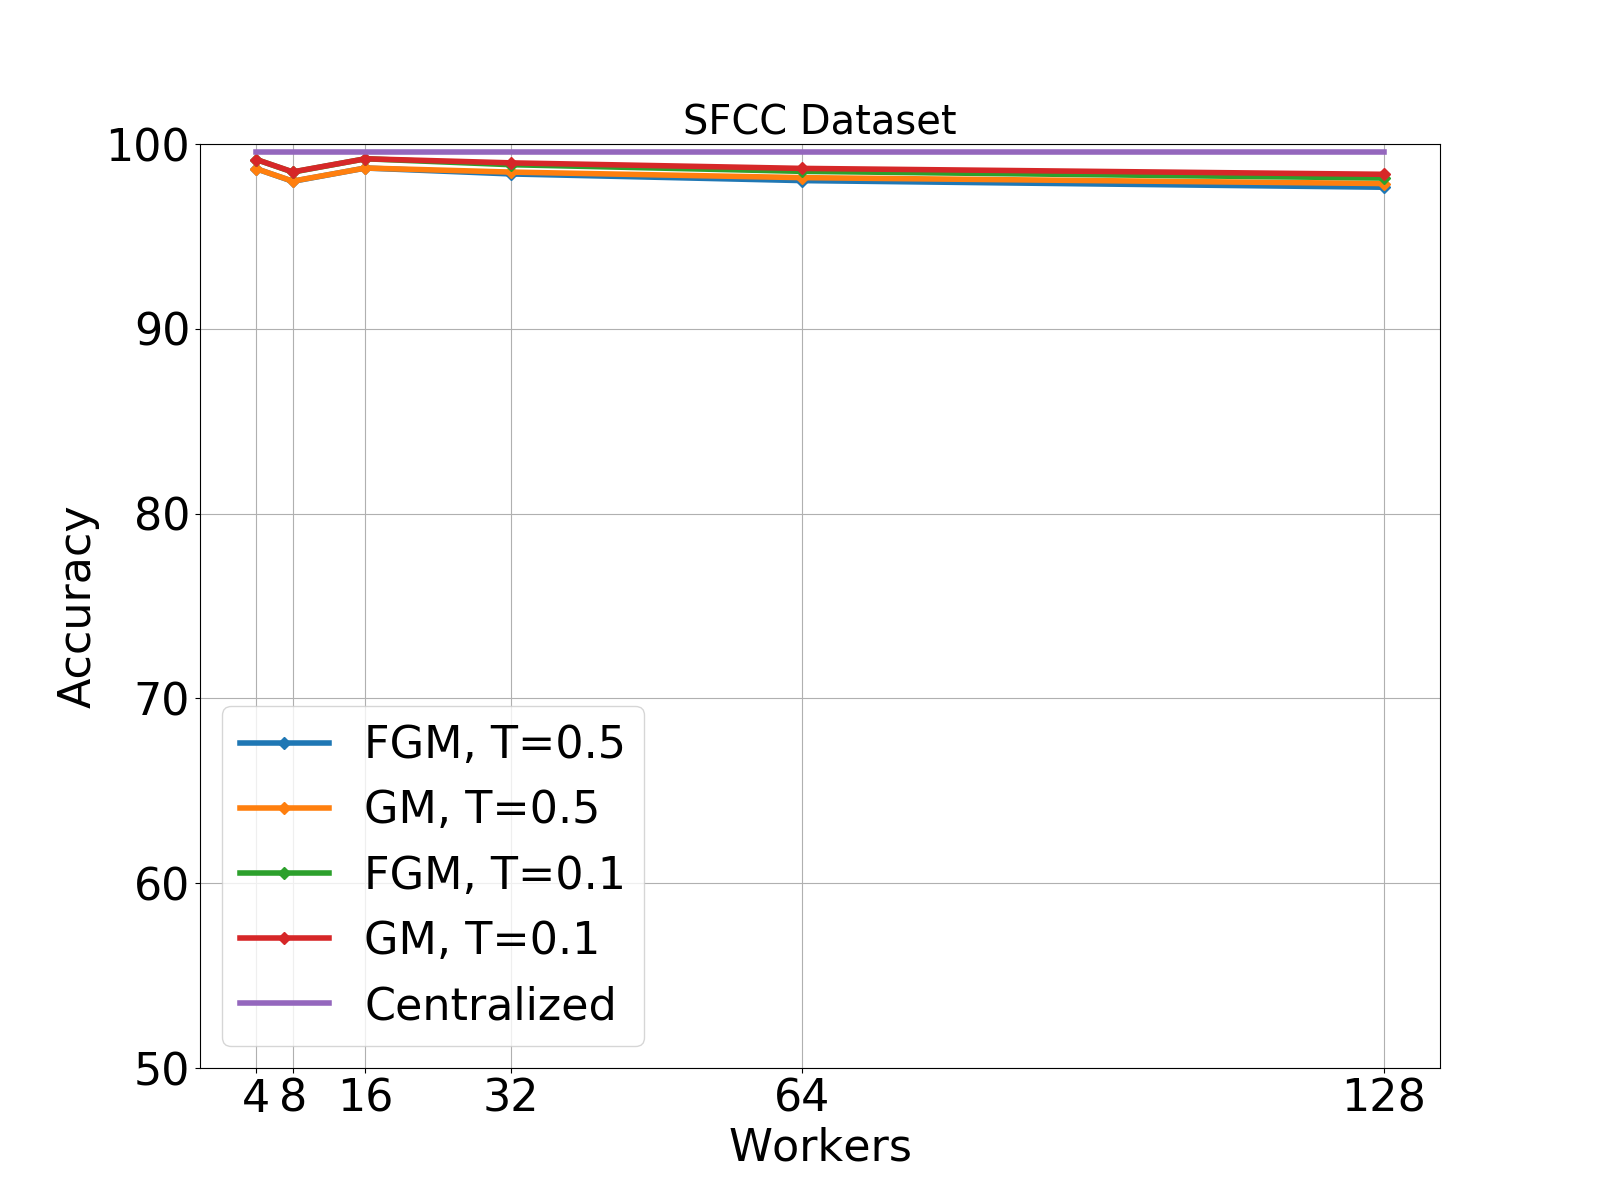
\includegraphics[width=5.2cm,height=3.7cm]{./images/results/sfc-plots/exp_Fig_3_1_b.png}}
        \subfigure{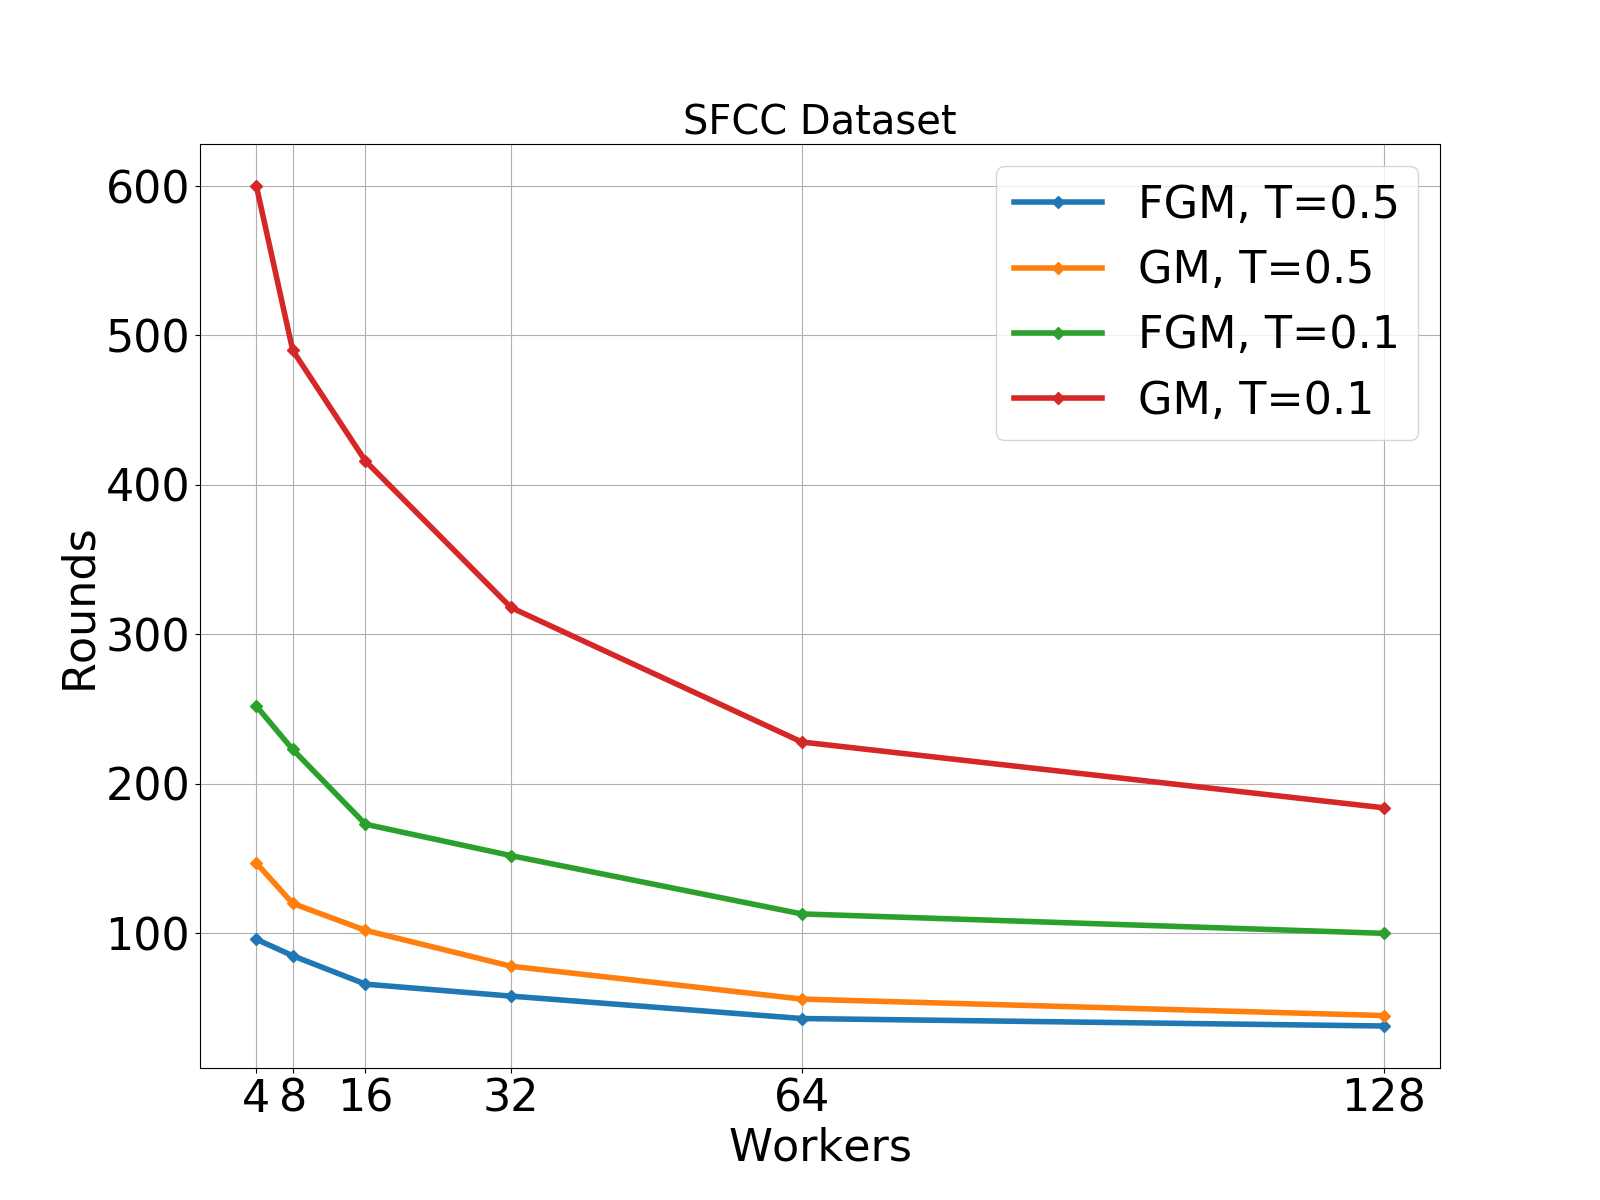
\includegraphics[width=5.2cm,height=3.7cm]{./images/results/sfc-plots/exp_Fig_3_2_b.png}}
        \subfigure{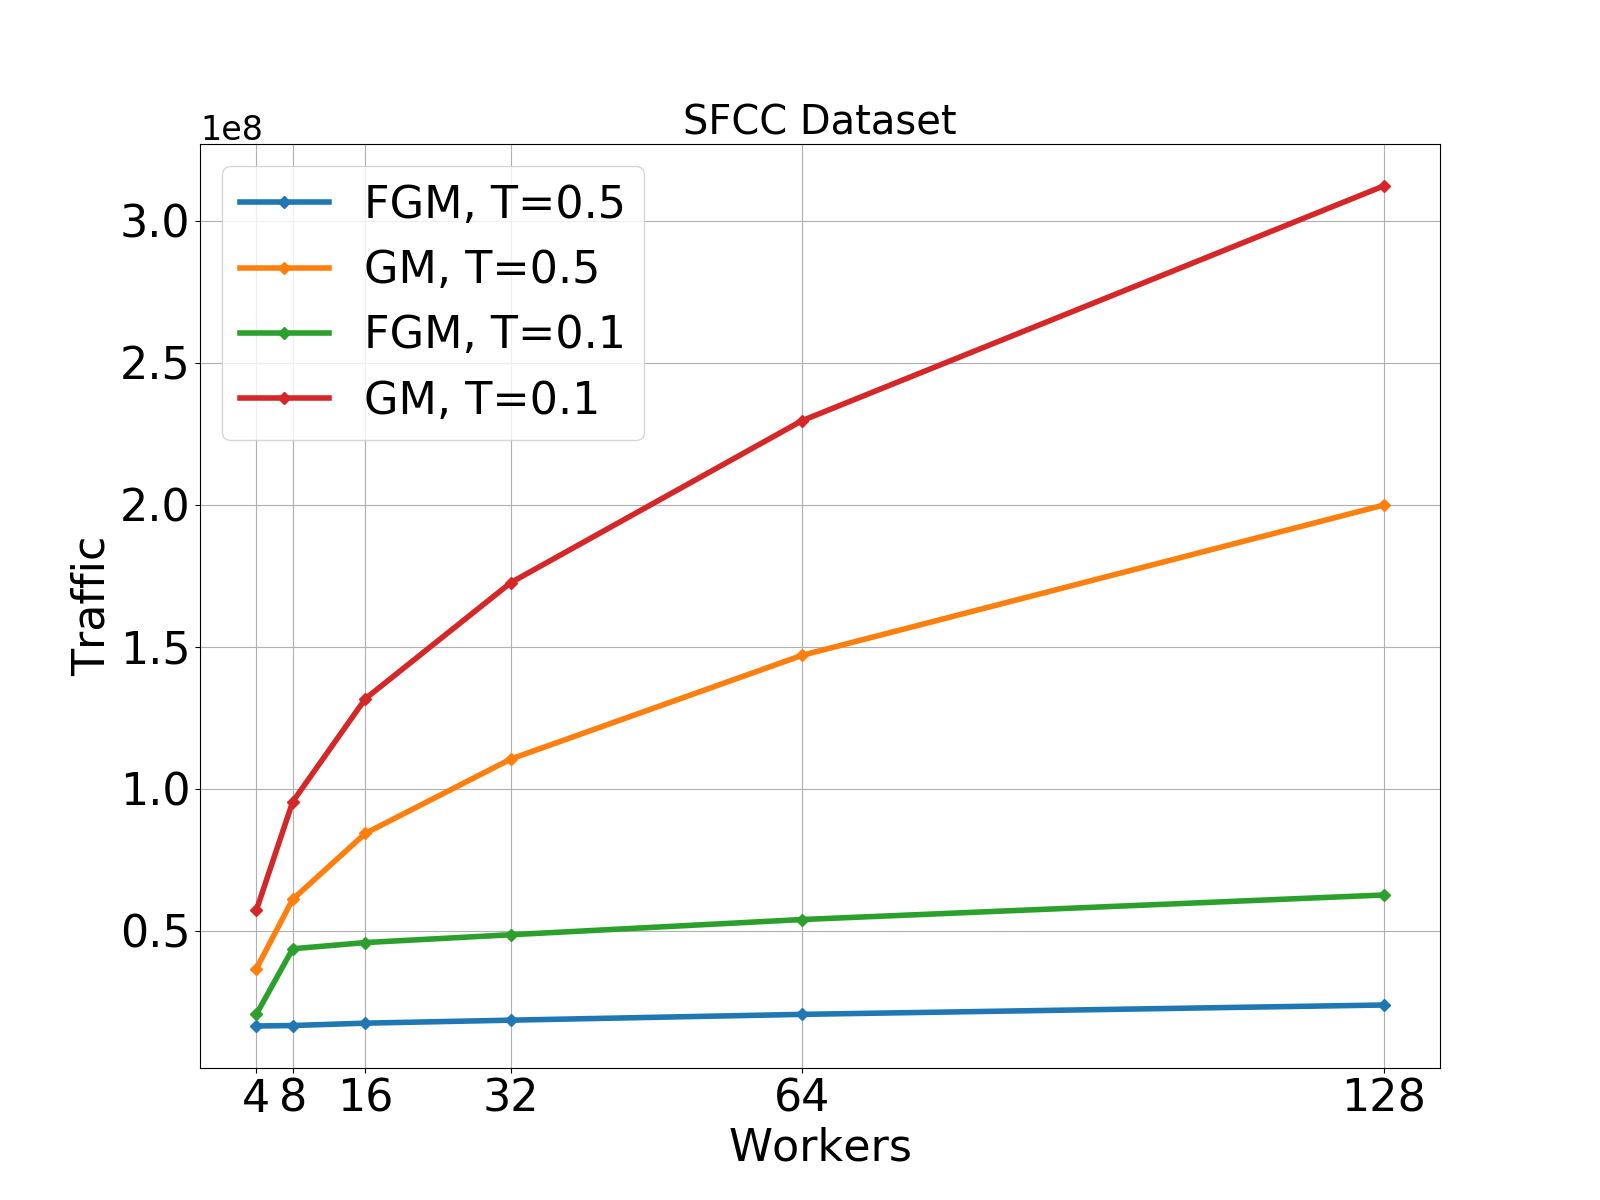
\includegraphics[width=5.2cm,height=3.7cm]{./images/results/sfc-plots/exp_Fig_3_3_b.png}}
        \label{fig:sfc_thres_workers}
    \end{figure}
\end{frame}

\subsection{Safe Functions Comparison}\label{subsec:safe-functions-comparison}

\begin{frame}{Safe Zone Problem}
    \setbeamertemplate{itemize items}[circle]
    \begin{itemize}
        \item{This time, we compare the two safe functions using the\\ \emph{same} protocol (\textbf{FGM}).}
        \item{The two safe functions are,}
        \vspace{0.2cm}
        \item[]{
        \begin{block}{Safe Function 1 (SF1) - \emph{'Simple norm'}}
            $\phi(\pmb{X_i},\pmb{E}) = ||\pmb{X_i}-\pmb{E}||_2^2 - T$
        \end{block}}
        \vspace{0.3cm}
        \begin{block}{Safe Function 2 (SF2) - \emph{'Spherical cap'}}
            $\phi(\pmb{X_i},\pmb{E}) = \max\{-T||\pmb{E}|| - \pmb{X_i}\frac{\pmb{E}}{\pmb{||E||}}, ||\pmb{X_i}+\pmb{E}|| - (1+T)||\pmb{E}||\}$
        \end{block}
    \end{itemize}
\end{frame}

\begin{frame}{Results (1) - Changing the threshold ($\pmb{T}$)}
    \begin{itemize}
        \centering
        \item[]{\lbrack mini-batch=$16$, workers=$8$\rbrack}
    \end{itemize}
    \vspace{-0.3cm}
    \begin{figure}
        \subfigure{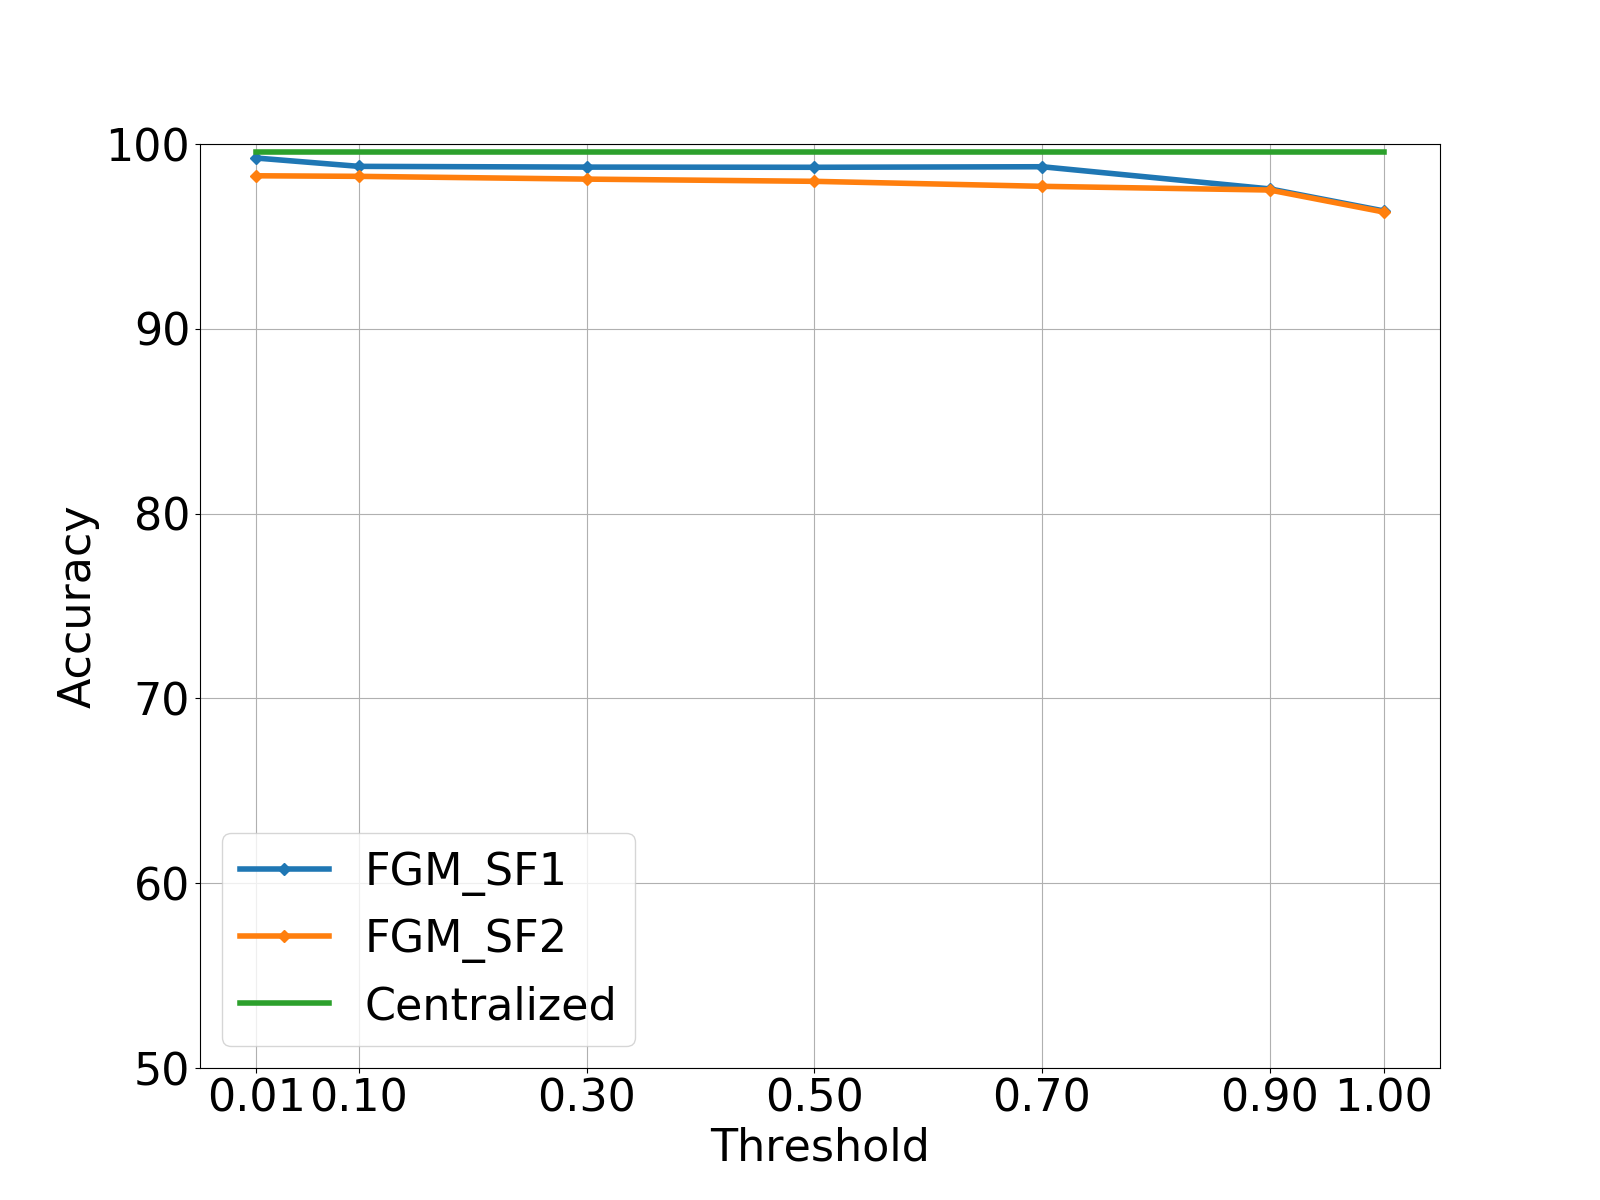
\includegraphics[width=5.2cm,height=3.7cm]{./images/results/sf-comp/exp_Fig_1_1.png}}
        \subfigure{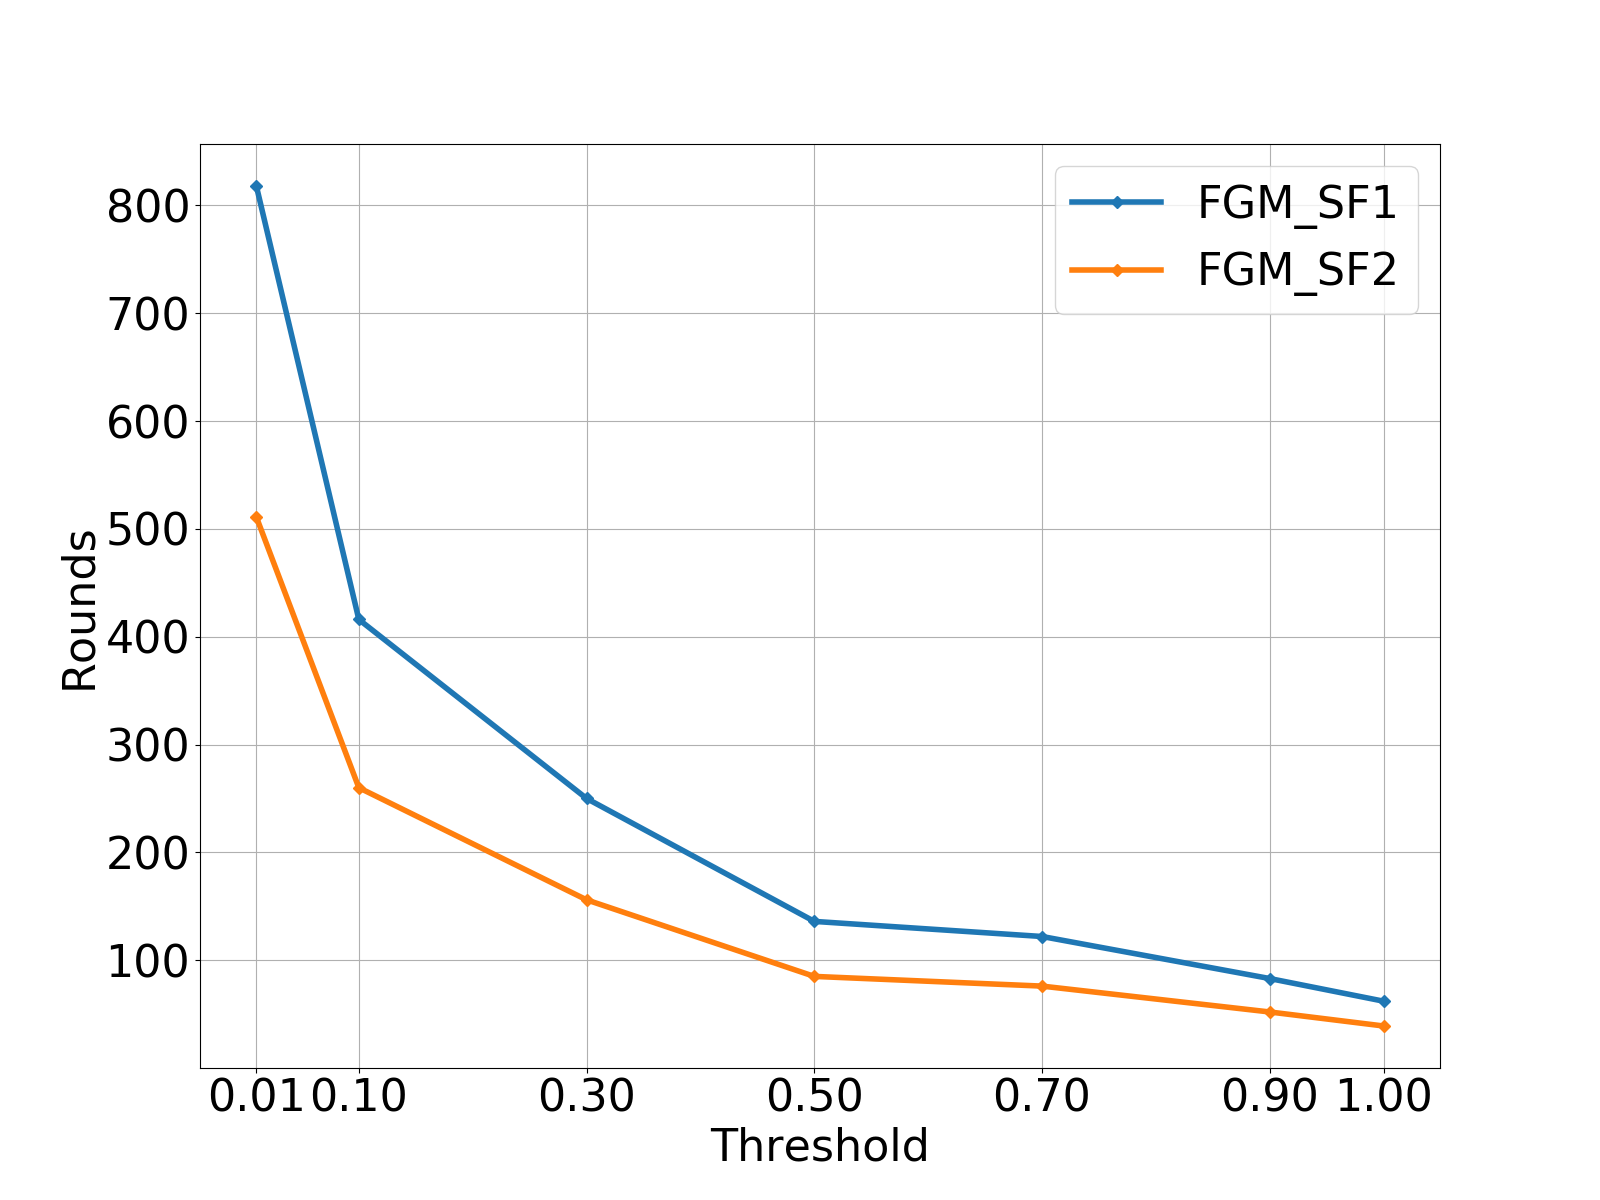
\includegraphics[width=5.2cm,height=3.7cm]{./images/results/sf-comp/exp_Fig_1_2.png}}
        \subfigure{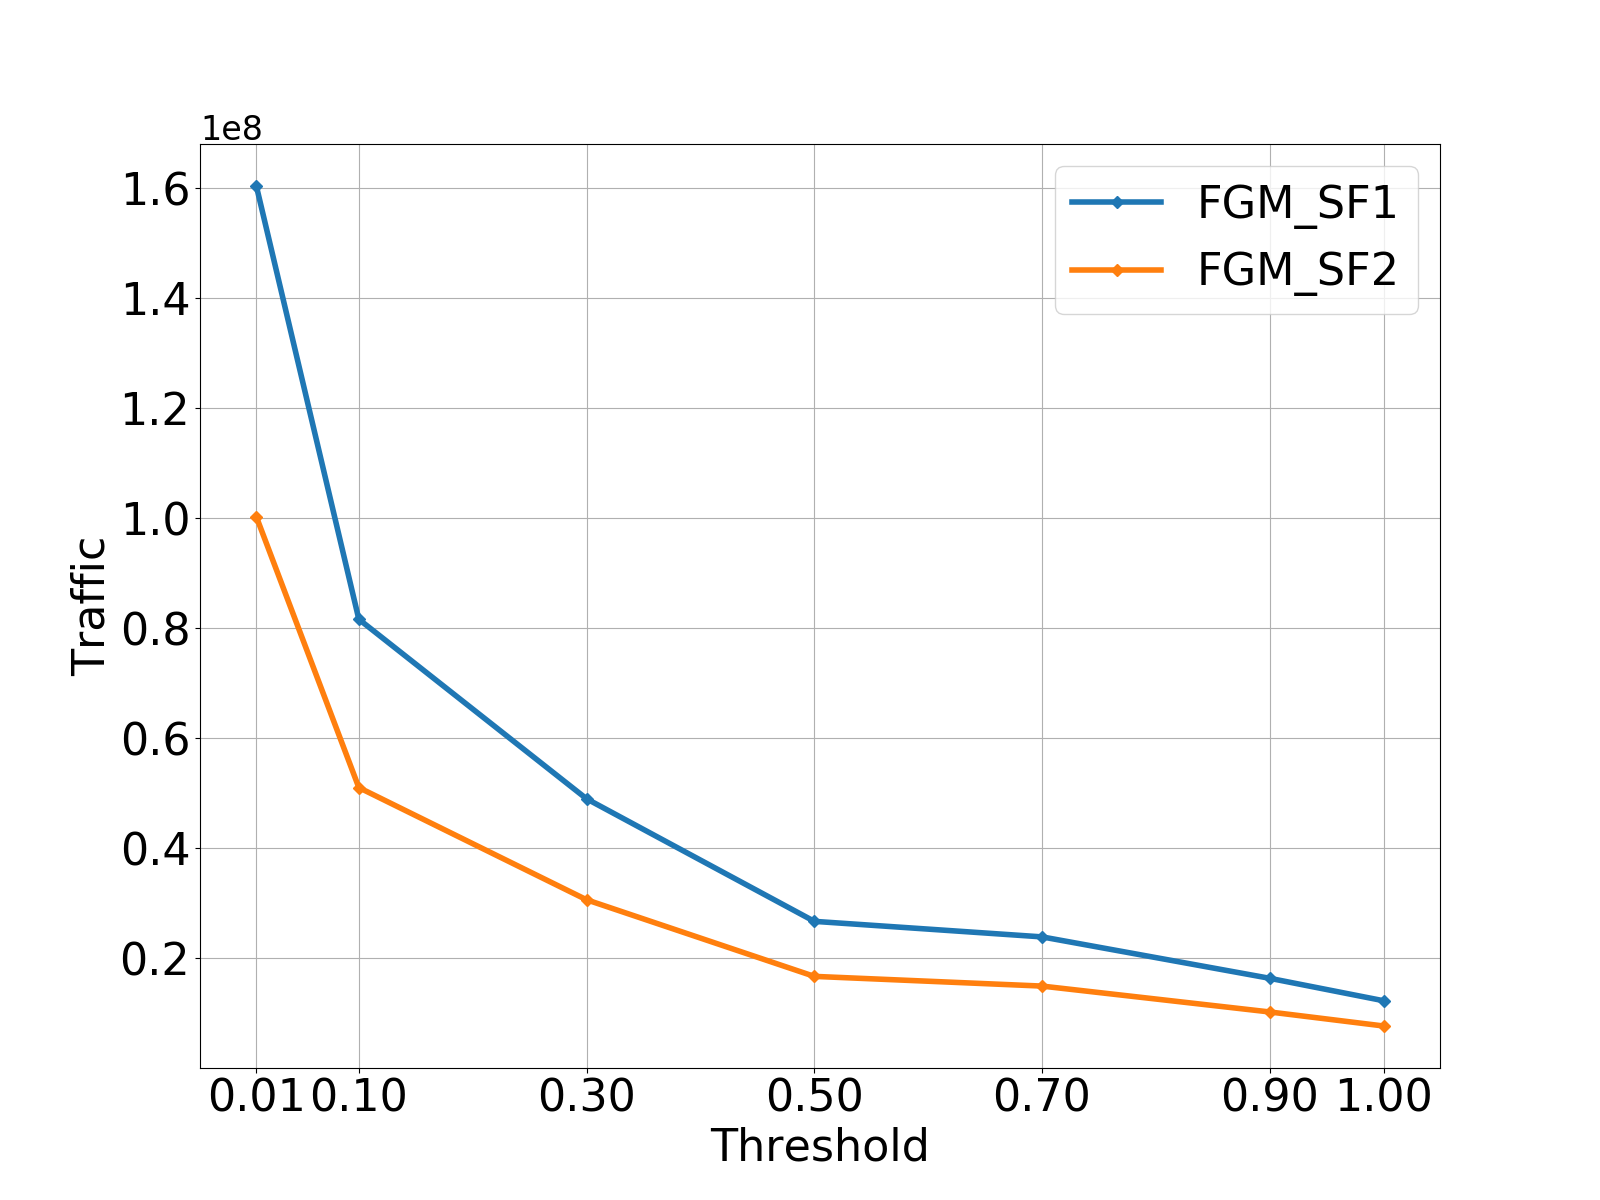
\includegraphics[width=5.2cm,height=3.7cm]{./images/results/sf-comp/exp_Fig_1_3.png}}
        \label{fig:sf_acc}
    \end{figure}
\end{frame}

\begin{frame}{Results (2) - Changing the mini-batch size ($\pmb{|\beta|}$)}
    \begin{itemize}
        \centering
        \item[]{\lbrack threshold=$0.5$, workers=$8$\rbrack}
    \end{itemize}
    \vspace{-0.3cm}
    \begin{figure}
        \subfigure{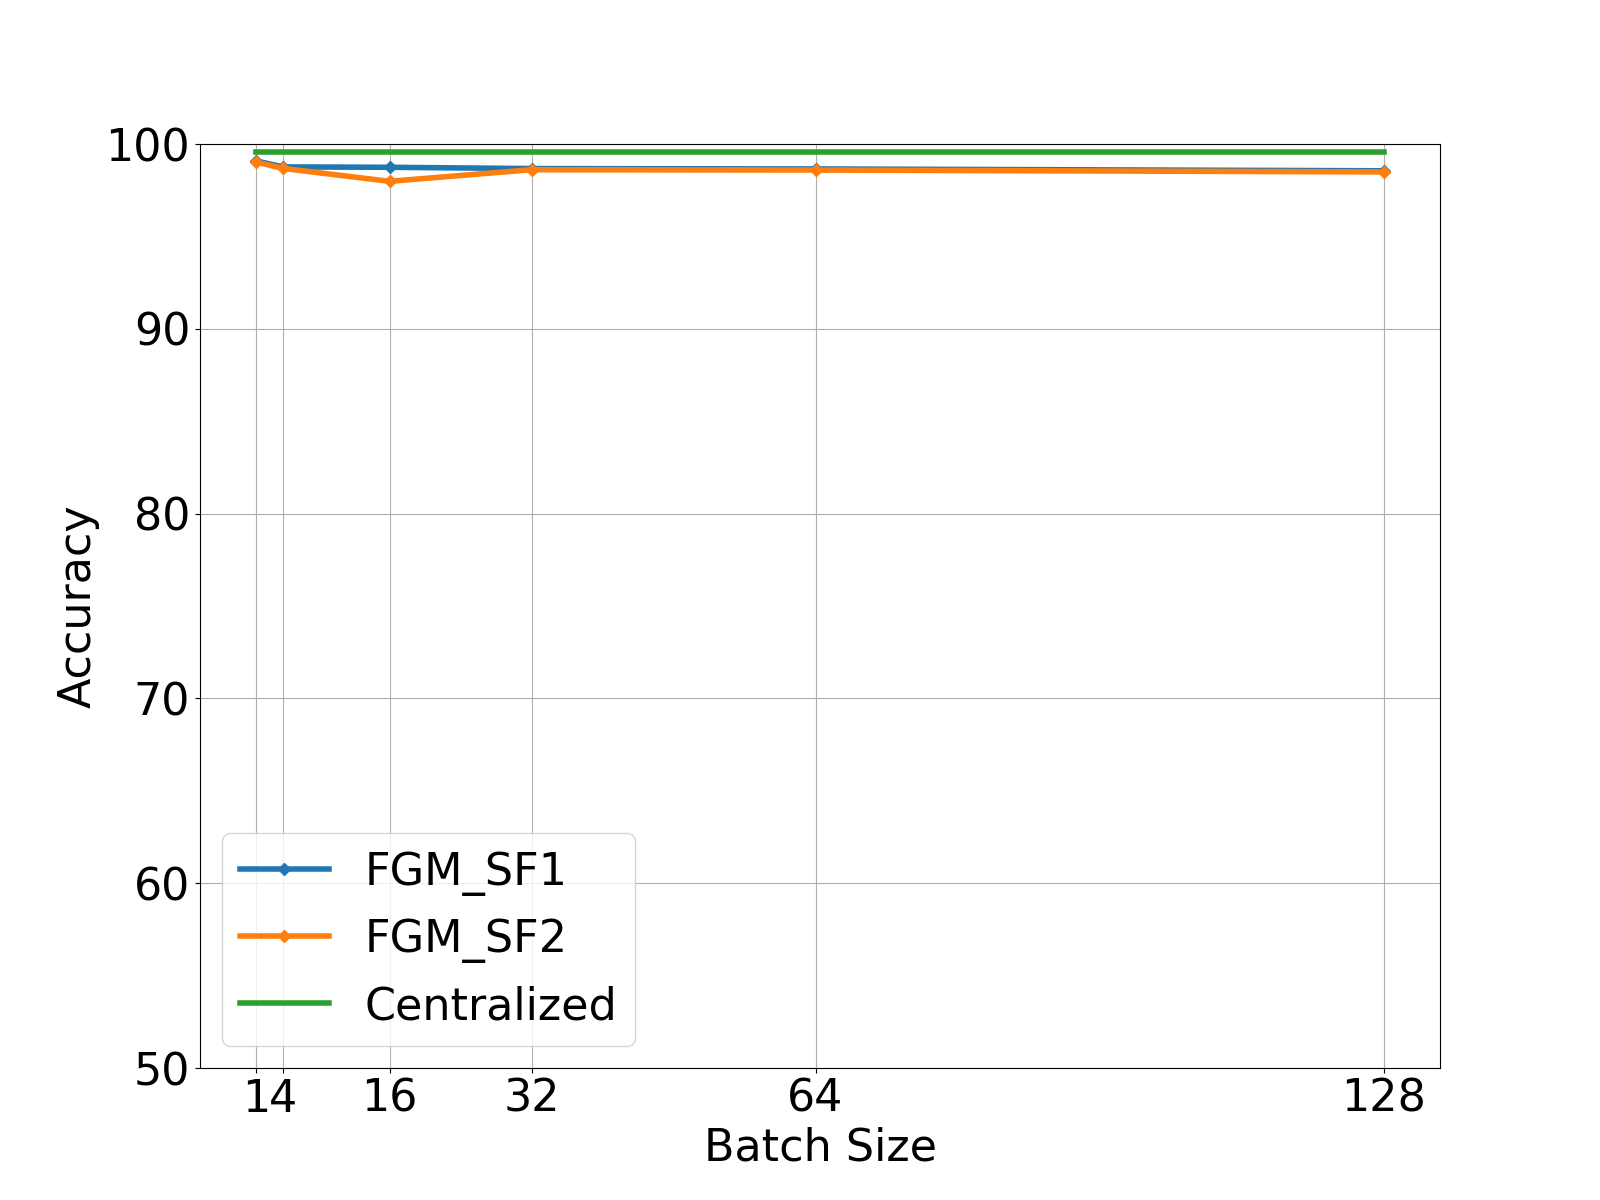
\includegraphics[width=5.2cm,height=3.7cm]{./images/results/sf-comp/exp_Fig_2_1.png}}
        \subfigure{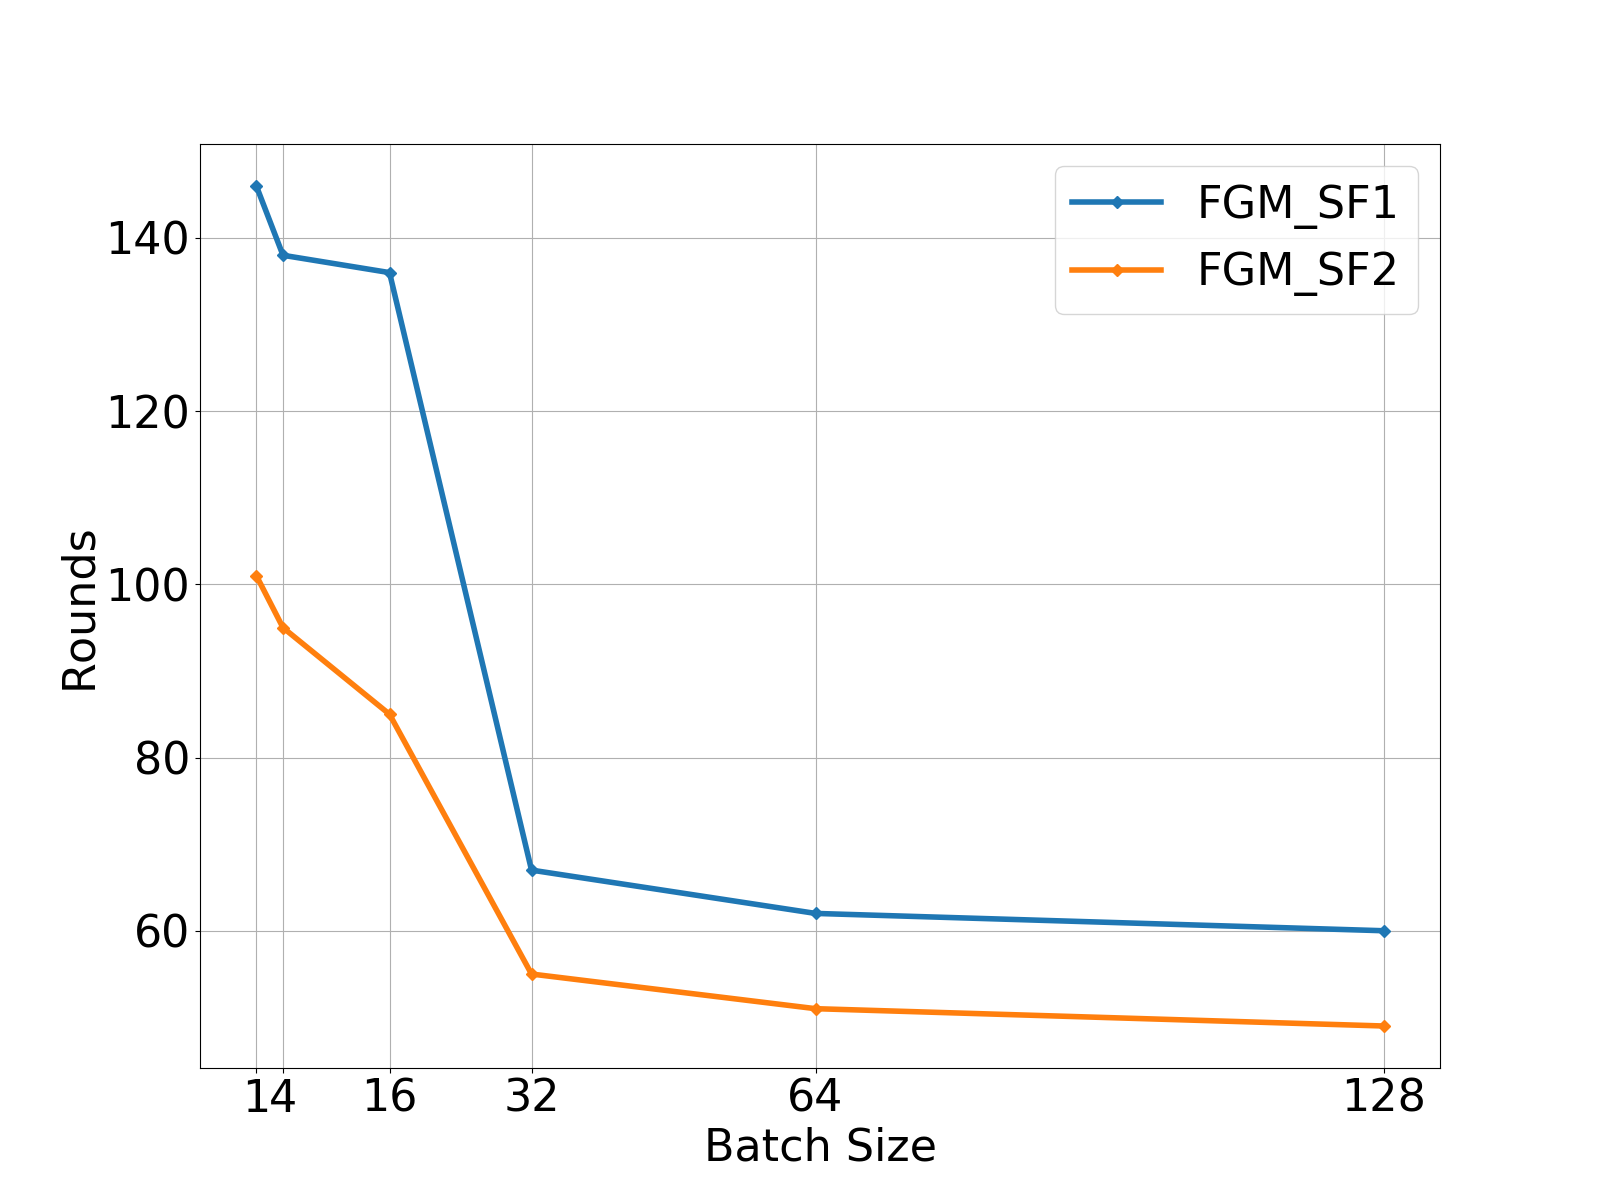
\includegraphics[width=5.2cm,height=3.7cm]{./images/results/sf-comp/exp_Fig_2_2.png}}
        \subfigure{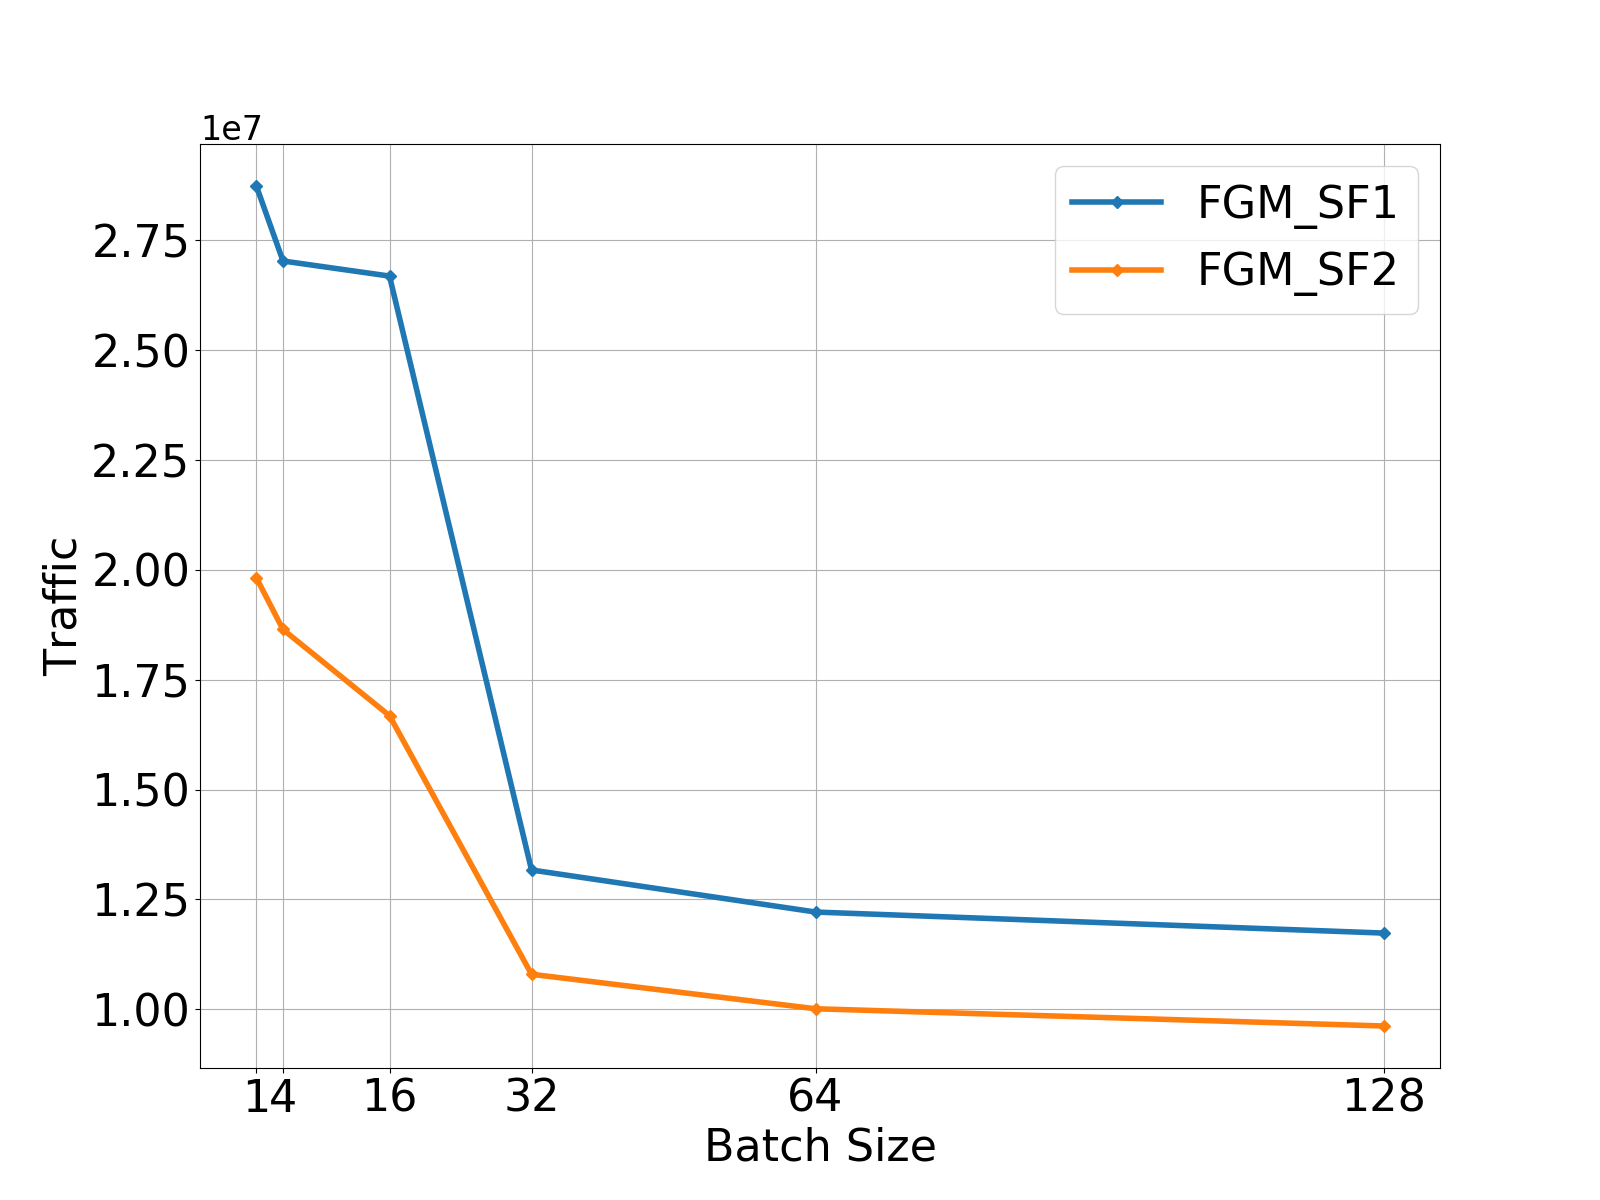
\includegraphics[width=5.2cm,height=3.7cm]{./images/results/sf-comp/exp_Fig_2_3.png}}
        \label{fig:sf_rnds}
    \end{figure}
\end{frame}

\begin{frame}{Results (3) - Changing the number of workers ($\pmb{n}$)}
    \begin{itemize}
        \centering
        \item[]{\lbrack threshold=$0.5$, mini-batch=$16$\rbrack}
    \end{itemize}
    \vspace{-0.3cm}
    \begin{figure}
        \subfigure{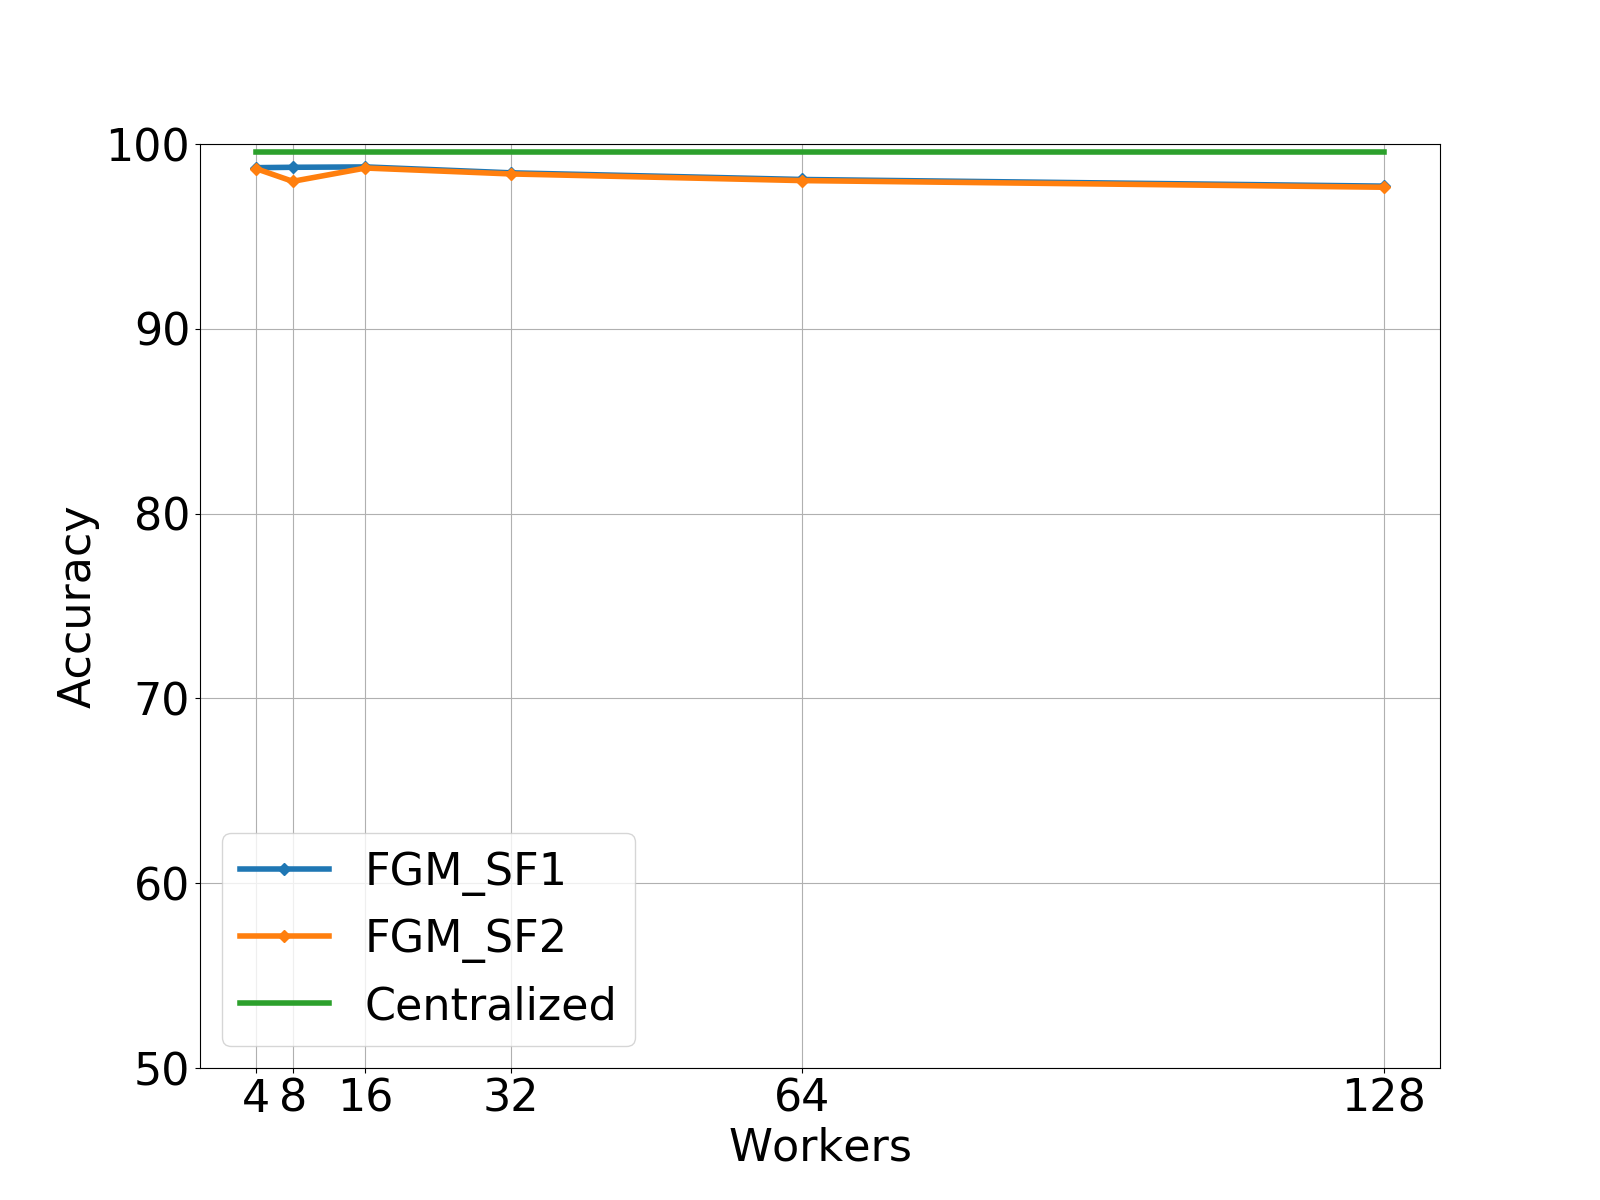
\includegraphics[width=5.2cm,height=3.7cm]{./images/results/sf-comp/exp_Fig_3_1.png}}
        \subfigure{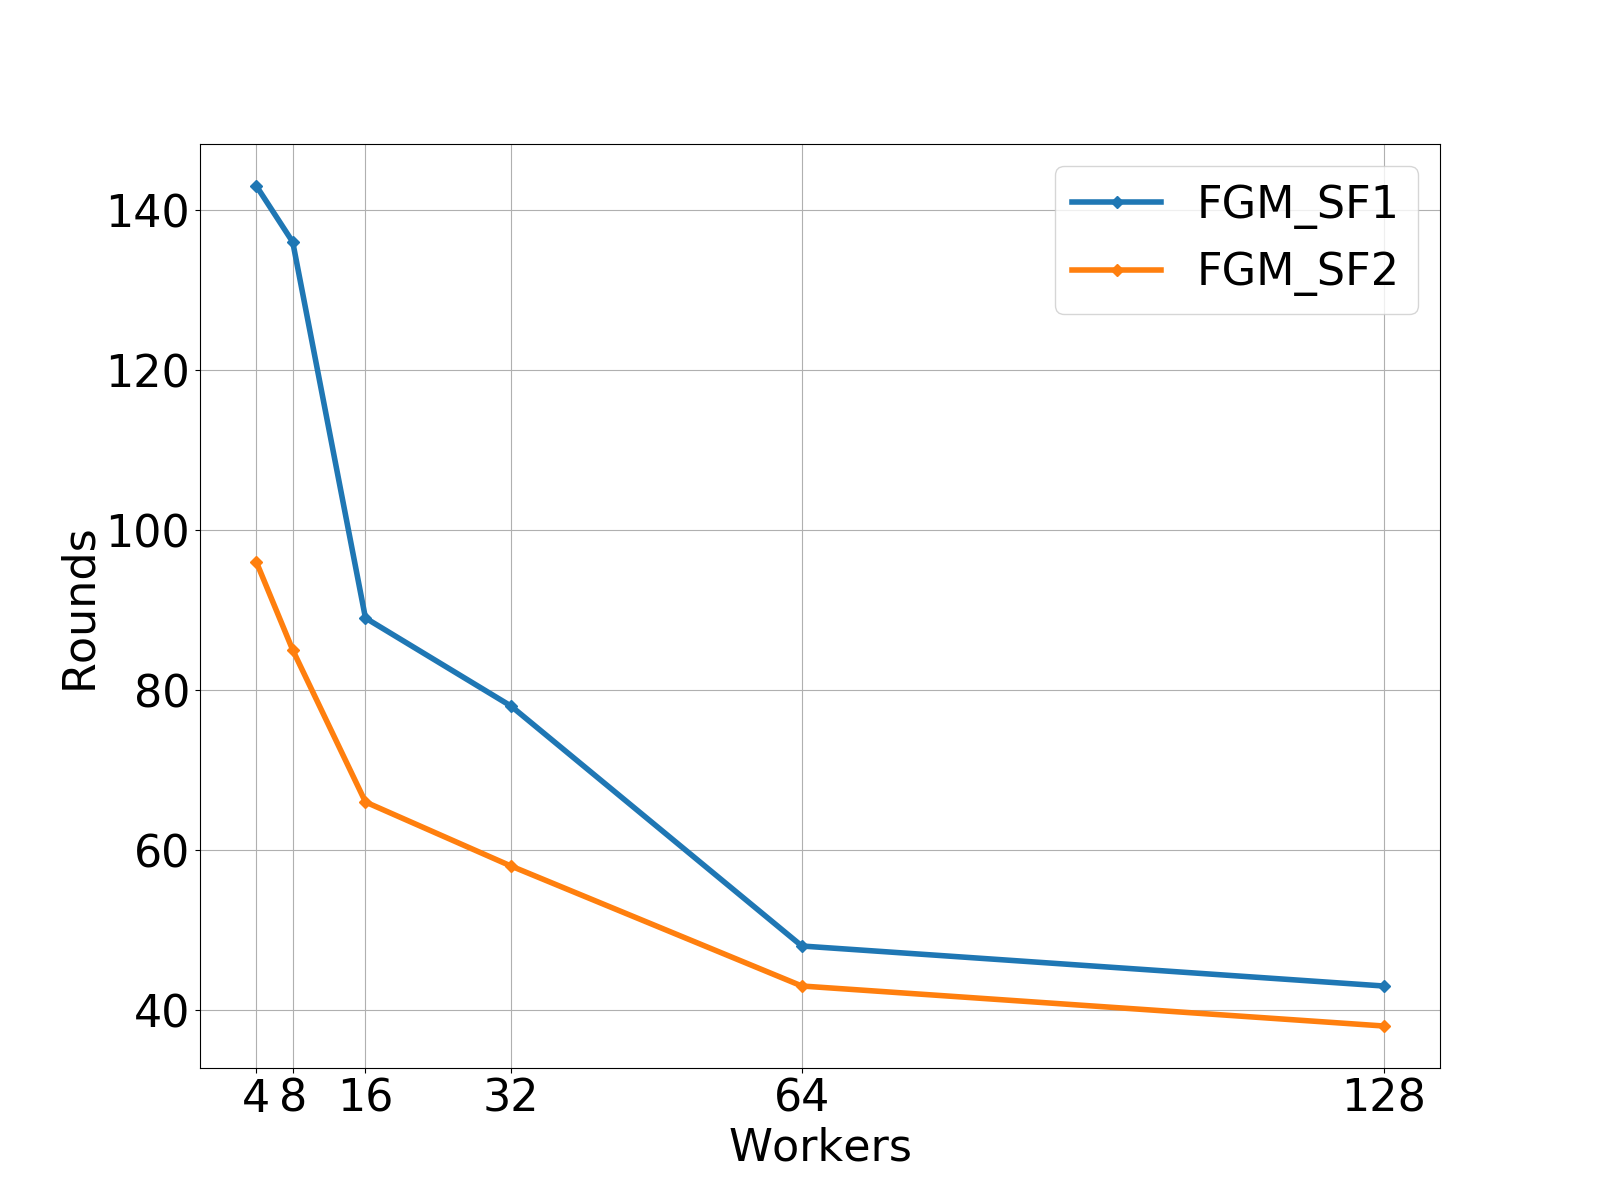
\includegraphics[width=5.2cm,height=3.7cm]{./images/results/sf-comp/exp_Fig_3_2.png}}
        \subfigure{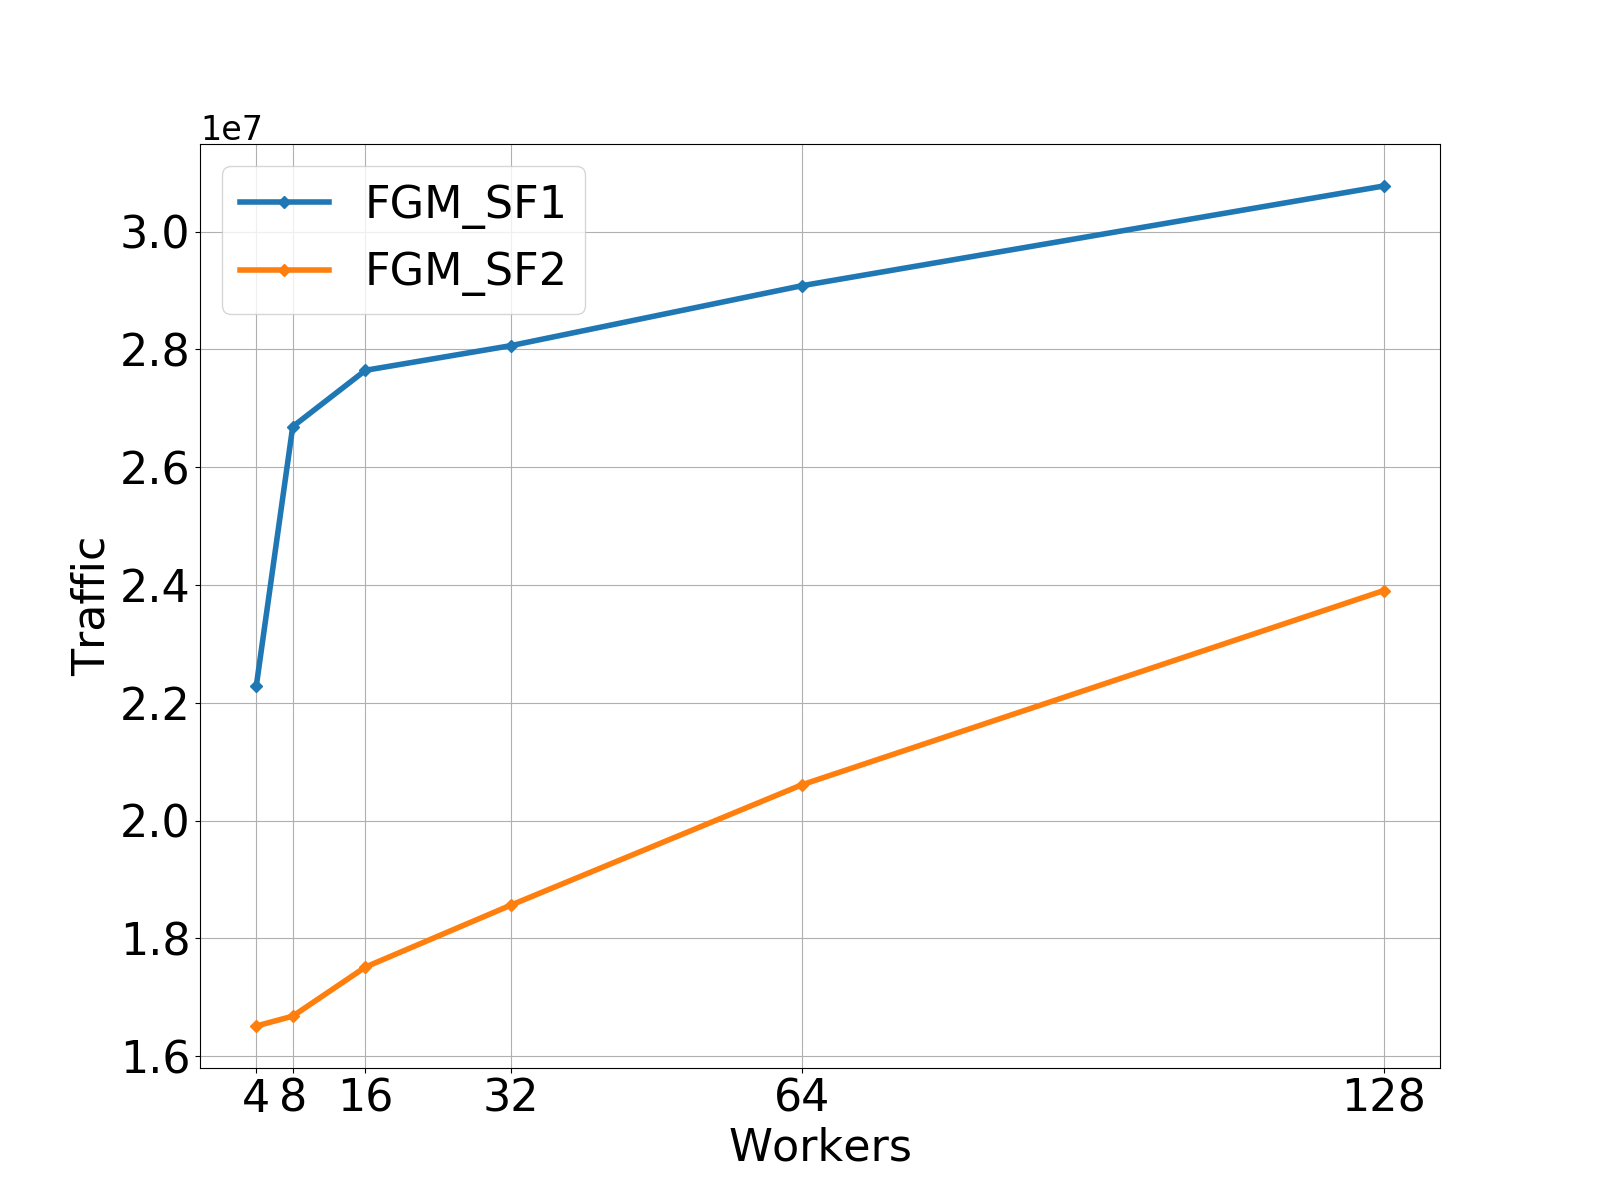
\includegraphics[width=5.2cm,height=3.7cm]{./images/results/sf-comp/exp_Fig_3_3.png}}
        \label{fig:sf_trff}
    \end{figure}
\end{frame}

    \section{Conclusion}\label{sec:conclusion}
    \chapter{Conclusions}\label{ch:conclusions}

\section{Contribution}\label{sec:conclusion}

Our recommended method for distributed DL achieves high predictive performance, yet needs essentially less communication than GM\@.
Furthermore, the method handles not only the learning algorithm but also the optimizer as black-boxes.
In this work, I proved that FGM is better than GM for distributed DL learning and especially using LSTM networks, a subset of the Recurrent Neural Networks.
I tested this architecture on solving two types of problems, classification, and sentiment analysis.
In both cases, the results were impressive.
But if we have to choose one of these two for which the architecture is more suitable, the answer is the NLP problem.
Taking into account the difficulty of both problems, our architecture reacted almost in the same way in both cases.

In the second phase, I compared the two functions with each other.
The results revealed that SF2 is much cheaper than SF1 in terms of network cost, but the latter achieves better accuracy on the prediction.
Of course, this difference is not so important as to make us prefer it.
Therefore, sacrificing minimal accuracy in the model, we choose SF2 as the best for distributed deep learning.

\section{Future Work}\label{sec:future-work}

In this work, I simulated a scenario calculating the network traffic cost of the training process of RNN by the GM and FGM protocol.
We know this time in practice that the FGM protocol is more efficient than GM.
Thus, a future direction would be an actual system that uses FGM to train these networks.
Recently, Sofia Kampioti~\cite{kampioti_sofia__thesis_2020} implemented such a system to train an ML model for classification purposes using the Support Vector Machines (SVM) algorithm.

Another future direction would be the usage of the rebalancing version of FGM on RNN training.
Using the rebalancing version, we can undoubtedly achieve much more efficient training concerning the network cost.

Last, in this project, we made offline learning.
Future work could attempt to make this process online, taking into consideration some meaning like Concept Drift.
An online learning algorithm can resolve some issues like concept changes.
To make this more specific, in this task I used the food reviews as training samples.
In an online learning system, we could change the concept of training samples to cloth reviews without accepting a large reduction in the forecast performance.


\end{document}
